% This is "sig-alternate.tex" V2.1 April 2013
% This file should be compiled with V2.5 of "sig-alternate.cls" May 2012
%
% This example file demonstrates the use of the 'sig-alternate.cls'
% V2.5 LaTeX2e document class file. It is for those submitting
% articles to ACM Conference Proceedings WHO DO NOT WISH TO
% STRICTLY ADHERE TO THE SIGS (PUBS-BOARD-ENDORSED) STYLE.
% The 'sig-alternate.cls' file will produce a similar-looking,
% albeit, 'tighter' paper resulting in, invariably, fewer pages.
%
% ----------------------------------------------------------------------------------------------------------------
% This .tex file (and associated .cls V2.5) produces:
%       1) The Permission Statement
%       2) The Conference (location) Info information
%       3) The Copyright Line with ACM data
%       4) NO page numbers
%
% as against the acm_proc_article-sp.cls file which
% DOES NOT produce 1) thru' 3) above.
%
% Using 'sig-alternate.cls' you have control, however, from within
% the source .tex file, over both the CopyrightYear
% (defaulted to 200X) and the ACM Copyright Data
% (defaulted to X-XXXXX-XX-X/XX/XX).
% e.g.
% \CopyrightYear{2007} will cause 2007 to appear in the copyright line.
% \crdata{0-12345-67-8/90/12} will cause 0-12345-67-8/90/12 to appear in the copyright line.
%
% ---------------------------------------------------------------------------------------------------------------
% This .tex source is an example which *does* use
% the .bib file (from which the .bbl file % is produced).
% REMEMBER HOWEVER: After having produced the .bbl file,
% and prior to final submission, you *NEED* to 'insert'
% your .bbl file into your source .tex file so as to provide
% ONE 'self-contained' source file.
%
% ================= IF YOU HAVE QUESTIONS =======================
% Questions regarding the SIGS styles, SIGS policies and
% procedures, Conferences etc. should be sent to
% Adrienne Griscti (griscti@acm.org)
%
% Technical questions _only_ to
% Gerald Murray (murray@hq.acm.org)
% ===============================================================
%
% For tracking purposes - this is V2.0 - May 2012

\documentclass[acmsmall]{acmart}
%\documentclass[prodmode,acmtecs]{acmart}
\usepackage{balance}  % for  \balance command ON LAST PAGE  (only there!)
\usepackage{algorithm}
\usepackage{epsfig}
\usepackage{graphicx}
\usepackage{esvect} % for arrows
\usepackage{xspace,multirow,amsmath, color,array,colortbl} %
\usepackage{subfigure}
\usepackage[english]{babel}
\usepackage[bigsqcap]{stmaryrd}
\usepackage[normalem]{ulem}
%\usepackage{zi4,newtxmath}

%\usepackage{lmodern} %do not use lmodern, otherwise, brackets in equation will be lost.
%\usepackage{cite}

\newcommand{\imp}{\vdash_{\cal I}}


%%%%%%%%%%%%%%%%%%%%%%%%%%%%%%%%%%%%%%%%%%
% Enumerate and Itemize modifications
%\usepackage{enumitem}
%\setlist{topsep=0pt,noitemsep} \setitemize[1]{label=$\circ$}
%%%%%%%%%%%%%%%%%%%%%%%%%%%%%%%%%%%%%%%%%%%

\sloppy
\newcommand{\rtable}[1]{\ensuremath{\mathsf{#1}}}
\newcommand{\ratt}[1]{\ensuremath{\mathit{#1}}}
\newcommand{\at}[1]{\protect\ensuremath{\mathsf{#1}}\xspace}
\newcommand{\myhrule}{\rule[.5pt]{\hsize}{.5pt}}
\newcommand{\oneurl}[1]{\texttt{#1}}
\newcommand{\eat}[1]{}
\newcommand{\stab}{\rule{0pt}{8pt}\\[-1.6ex]}
\newcommand{\sttab}{\rule{0pt}{8pt}\\[-2ex]}
%\newcommand{\sstab}{\rule{0pt}{8pt}\\[-2.4ex]}
\newcommand{\tabstrut}{\rule{0pt}{4pt}\vspace{-0.07in}}
\newcommand{\vs}{\vspace{1ex}}
\newcommand{\exa}[2]{{\tt\begin{tabbing}\hspace{#1}\=\+\kill #2\end{tabbing}}}
\newcommand{\ra}{\rightarrow}
\newcommand{\la}{\leftarrow}
\newcommand{\bi}{\begin{itemize}}
\newcommand{\ei}{\end{itemize}}
\newenvironment{tbi}{\begin{itemize}
        \setlength{\topsep}{1.5ex}\setlength{\itemsep}{0ex}\vspace{-0.5ex}}
        {\end{itemize}\vspace{-0.5ex}}
\newenvironment{tbe}{\begin{enumerate}
        \setlength{\topsep}{0ex}\setlength{\itemsep}{-0.7ex}\vspace{-1ex}}
        {\end{itemize}\vspace{-1ex}}

\newcommand{\mat}[2]{{\begin{tabbing}\hspace{#1}\=\+\kill #2\end{tabbing}}}
\newcommand{\m}{\hspace{0.05in}}
\newcommand{\ls}{\hspace{0.1in}}
\newcommand{\be}{\begin{enumerate}}
\newcommand{\ee}{\end{enumerate}}
\newcommand{\beqn}{\begin{eqnarray*}}
\newcommand{\eeqn}{\end{eqnarray*}}
\newcommand{\card}[1]{\mid\! #1\!\mid}
\newcommand{\fth}{\hfill $\Box$}
\newcommand{\AND}{\displaystyle{\bigwedge_{i=1}^{n}}}
%\newcommand{\U}[1]{\displaystyle{\bigcup_{#1}}}
\newcommand{\Sm}[1]{\displaystyle{\sum_{#1}}}
\newcommand{\stitle}[1]{\vspace{1ex}\noindent{\bf #1}}
\newcommand{\etitle}[1]{\vspace{0.5ex}\noindent{\em \underline{#1}}}
\renewcommand{\t}{\tau}
\newcommand{\Inh}[1]{\$#1}
\renewcommand{\r}[1]{{\it rule}(#1)}
\newcommand{\pa}{\parallel}
\newcommand{\LHS}{\kw{{\small LHS}}}
\newcommand{\RHS}{\kw{RHS}}
\newcommand{\len}{\kw{len}}
\newcommand{\kop}{\kw{op}}
%\newcommand{\st}{\emph{s.t.}\xspace}
\newcommand{\ie}{\emph{i.e.,}\xspace}
\newcommand{\eg}{\emph{e.g.,}\xspace}
\newcommand{\wrt}{\emph{w.r.t.}\xspace}
\newcommand{\aka}{\emph{a.k.a.}\xspace}
\newcommand{\kwlog}{\emph{w.l.o.g.}\xspace}

\newcommand{\VNM}{\kw{VNM}}
\newcommand{\VNMs}{\kw{VNM}}
\newcommand{\VN}{\kw{VN}}
\newcommand{\SN}{\kw{SN}}

%%%%%%%%%%%%%%%%%%%%%%%%%%%%%%%%%%%%%%%%%%%%%%%%%%%%%%%%%%%%%%%%
%                  Relation Algebra operators
%%%%%%%%%%%%%%%%%%%%%%%%%%%%%%%%%%%%%%%%%%%%%%%%%%%%%%%%%%%%%%%%

\newcommand{\RS}{{\small S}\xspace}
\newcommand{\RP}{{\small P}\xspace}
\newcommand{\RJ}{{\sc j}\xspace}
\newcommand{\RC}{{\small C}\xspace}
\newcommand{\RSJ}{{\small SJ}\xspace}
\newcommand{\RSC}{{\small SC}\xspace}
\newcommand{\RSP}{{\small SP}\xspace}
\newcommand{\RPJ}{{\small PJ}\xspace}
\newcommand{\RPC}{{\small PC}\xspace}
\newcommand{\RSPJ}{{\sc spj}\xspace}
\newcommand{\RSPC}{{\small SPC}\xspace}
\newcommand{\RSPJU}{{\sc spju}\xspace}
\newcommand{\RSPCU}{{\small SPCU}\xspace}
\newcommand{\RSPJUN}{{\small SPJU$^N$}\xspace}
\newcommand{\RSPCUN}{{\small SPCU$^N$}\xspace}
%%%%%%%%%%%%%%%%%%%%%%%%%%%%%%%%%%%%%%%%%%%%%%%%%%%%%%%%%%%%%%%%%%%%%%%%%%%%%%
% ALGORITHMS
%%%%%%%%%%%%%%%%%%%%%%%%%%%%%%%%%%%%%%%%%%%%%%%%%%%%%%%%%%%%%%%%%%%%%%%%%%%%%%%
\newcommand{\kw}[1]{{\ensuremath {\mathsf{#1}}}\xspace}

\newcounter{ccc}
\newcommand{\bcc}{\setcounter{ccc}{1}\theccc.}
\newcommand{\icc}{\addtocounter{ccc}{1}\theccc.}
\newcommand{\checking}{{\mbox{\small\sf Checking}\xspace}}
\newcommand{\preProcessing}{{\mbox{\small\sf preProcessing}\xspace}}
\newcommand{\CFDconsistency}{{\mbox{\small\sf CFD\_Checking}\xspace}}
\newcommand{\MCS} {\kw{MCS}}
\newcommand{\templateDB}{{\mbox{\small\sf templateDB}\xspace}}
\newcommand{\ChaseChecking}{{\mbox{\small\sf RandomChecking}\xspace}}
\newcommand{\chase}{{\mbox{\small\sf Chase}\xspace}}
\newcommand{\SAT}{{\mbox{\small\sf SAT}\xspace}}
\newcommand{\kSAT}{{\mbox{\small 3SAT}\xspace}}
\newcommand{\PropCFDSPC}{\kw{Prop{\small CFD\_SPC}}}
\newcommand{\PropCFDSPCU}{\kw{Prop{\small CFD\_SPCU}}}
\newcommand{\UnionEQs}{\kw{UnionEQs}}
\newcommand{\UnionCFDs}{\kw{UnionCFDs}}
\newcommand{\EQ}{\kw{EQ}}
\newcommand{\eq}{\kw{eq}}
\newcommand{\key}{\kw{key}}
\newcommand{\rep}{\kw{rep}}
\newcommand{\PEQ}{\kw{EQ2CFD}}
\newcommand{\Drop}{\kw{Drop}}
%\newcommand{\Res}{\kw{Res}}
\newcommand{\CFD}{{\small CFD}\xspace}
\newcommand{\CFDs}{{\small CFD}{\small s}\xspace}
\newcommand{\CIND}{{\sc cind}\xspace}
\newcommand{\cind}{{\small \sf CIND}}
\newcommand{\cfd}{{\small \sf CFD}}
\newcommand{\CINDp}{{\sc cind}$^+$\xspace}
\newcommand{\CINDn}{{\sc cind}$^-$\xspace}
\newcommand{\CINDs}{{\sc cind}{\small s}\xspace}
\newcommand{\FD}{{\small FD}\xspace}
\newcommand{\FDs}{{\small FD}{\small s}\xspace}
\newcommand{\IND}{{\sc ind}\xspace}
\newcommand{\INDs}{{\sc ind}{\small s}\xspace}
\newcommand{\TGDs}{{\sc tgd}{\small s}\xspace}
\newcommand{\NP}{{\small NP}\xspace}
\newcommand{\DTIME}{{\small DTIME}\xspace}
\newcommand{\NPO}{{\small NPO}\xspace}
\newcommand{\APX}{{\small APX}\xspace}
\newcommand{\DAGs}{{\sc dag}s\xspace}
\newcommand{\NC}{{\sc nc}\xspace}
\newcommand{\coNP}{co{\small NP}\xspace}
\newcommand{\PTIME}{{\small PTIME}\xspace}
\newcommand{\PSPACE}{{\sc pspace}\xspace}
\newcommand{\EXPTIME}{{\sc exptime}\xspace}
\newcommand{\NPSPACE}{{\sc npspace}\xspace}
\newcommand{\dom}{\protect\ensuremath{\mathsf{dom}}\xspace}
\newcommand{\atset}{\protect\ensuremath{\mathsf{attr}}\xspace}
\newcommand{\attr}[1]{\protect\ensuremath{\mathsf{#1}}\xspace}
\newcommand{\attrset}{\protect\ensuremath{\mathsf{attr}}\xspace}
\newcommand{\finatset}{\protect\ensuremath{\mathsf{finattr}}\xspace}
\newcommand{\pvar}{\protect\ensuremath{\mathsf{var\%}}\xspace}
\newcommand{\lLHS}{\protect\ensuremath{\mathsf{{\small LHS}}}\xspace}
\newcommand{\RA}{{\small RA}\xspace}
\newcommand{\RBR}{\kw{RBR}}
\newcommand{\SQL}{{\sc sql}\xspace}
\newcommand{\XSLT}{{\sc xslt}\xspace}
\newcommand{\DBMS}{{\sc dbms}\xspace}
\newcommand{\ATG}{{\sc atg}\xspace}
\newcommand{\ATGs}{{\sc atg}{\small s}\xspace}
\newcommand{\EBI}{{\sc ebi}\xspace}
\newcommand{\GO}{{\sc go}\xspace}
\newcommand{\VEC}[1]{{\sc vec}(#1)}
\newcommand{\DAG}{{\sc dag}\xspace}
\newcommand{\XQ}{{\sc xq}\xspace}
\newcommand{\XQwc}{{\sc xq}$^{\scriptscriptstyle[*]}$\xspace}
\newcommand{\XQdes}{{\sc xq}$^{\scriptscriptstyle[//]}$\xspace}
\newcommand{\XQfull}{{\sc xq}$^{\scriptscriptstyle[*,//]}$\xspace}
\newcommand{\vect}[1]{$\langle$ #1 $\rangle$}
\newcommand{\sem}[1]{[\![#1]\!]}
\newcommand{\NN}[2]{#1\sem{#2}}
\newcommand{\e}[2]{{\mathit (#1,#2)}}
\newcommand{\ep}[2]{{\mathit (#1,#2)+}}
\newcommand{\brname}{\ensuremath{{\mathsf{N}}}}
\newcommand{\budrel}[1]{\ensuremath{{\brname_{#1}}}}
\newcommand{\budgen}[2]{\ensuremath{Q^\brname_\e{#1}{#2}}}
\newcommand{\budcut}[2]{\ensuremath{Q_\e{#1}{#2}}}
\newcommand{\eop}{\hspace*{\fill}\mbox{$\Box$}}     % End of proof
\newcounter{example}%[section]
%\newcommand{\theexample}{\arabic{example}}
\newenvironment{example}{
         \vspace{1.5ex}
         \refstepcounter{example}
         {\noindent\bf Example \theexample:}}{
         \eop\vspace{1.5ex}}
\def\copyrightspace{}
\renewcommand{\ni}{\noindent}
\newcommand{\comlore}[1]{\begin{minipage}{3in}\fbox{\fbox{\parbox[t]{3in}{{\vspace{2mm}\noindent \bf COMM(LORE):~
{ #1}\hfill  END.}}}}\end{minipage}\\}
\newcommand{\comwenfei}[1]{\begin{minipage}{3in}\fbox{\fbox{\parbox[t]{3in}{{\vspace{2mm}\noindent \bf COMM(WENFEI):~
{ #1}\hfill  END.}}}}\end{minipage}\\}
\newcommand{\comshuai}[1]{\begin{minipage}{3in}\fbox{\fbox{\parbox[t]{3in}{{\vspace{2mm}\noindent \bf COMM(SHUAI):~
{ #1}\hfill  END.}}}}\end{minipage}\\}
\newcommand{\nthesection}{\arabic{section}}
%\newcounter{problem}
%\newenvironment{problem}{\begin{em}
%        \refstepcounter{problem}
%        {\vspace{1.5ex} \noindent\bf Problem \theproblem:}}{
%        \end{em}\eop\vspace{1.5ex}}
\newcounter{prop}[section]
%\renewcommand{\theprop}{\arabic{theorem}}
%\newcounter{lemma}[section]
%\renewcommand{\thelemma}{\arabic{theorem}}
%\newcounter{cor}[section]
%\renewcommand{\thecor}{\arabic{theorem}}
\newenvironment{ttheorem}{\begin{em}
         \refstepcounter{theorem}
         {\vspace{1.5ex} \noindent\bf  Theorem  \thetheorem:}}{
        \end{em}\eop\vspace{1.5ex}} %\hspace*{\fill}\vspace*{1ex}}
\newenvironment{pprop}{\begin{em}
        \refstepcounter{theorem}
        {\vspace{1.5ex}\noindent \bf Proposition \thetheorem:}}{
        \end{em}\eop\vspace{1.5ex}}%\hspace*{\fill}\vspace*{1ex}}
\newenvironment{llemma}{\begin{em}
         \refstepcounter{theorem}
        {\vspace{1.5ex}\noindent\bf Lemma \thetheorem:}}{
         \end{em}\eop\vspace{1.5ex}} %\hspace*{\fill}\vspace*{1ex}}
\newenvironment{cor}{\begin{em}
        \refstepcounter{theorem}
        {\vspace{1.5ex}\noindent\bf Corollary \thetheorem:}}{
        \end{em}\eop\vspace{1.5ex}} %\hspace*{\fill}\vspace*{1ex}}

%\newcounter{definition}
%\renewcommand{\thedefinition}{\arabic{definition}}
%\newenvironment{definition}{
%        \vspace{1.5ex}
%        \refstepcounter{definition}
%        {\noindent\bf Definition {\bf \thedefinition}:}}{\eop\vspace{1.5ex}
%}
\newcounter{alg}[section]
\renewcommand{\thealg}{\nthesection.\arabic{alg}}
\newenvironment{alg}[1]{
        \refstepcounter{alg}
        {\vspace{1ex}\noindent\bf Algorithm \thealg:\, #1}}{
        \vspace*{1ex}}
\newcounter{arule}
\renewcommand{\thearule}{\arabic{arule}}
\newenvironment{arule}{
        \vspace{0.6ex}
        \refstepcounter{arule}
        {\noindent \em Rule \thearule:}}{
        }
\newcounter{claim}
\renewcommand{\theclaim}{\arabic{claim}}
\newenvironment{claim}{
        \vspace{0.6ex}
        \refstepcounter{claim}
        {\noindent\em Claim \theclaim:}}{%--{ Wenfei Fan}\\
        }
\renewenvironment{proof}{
%\newenvironment{proof}{
        \vspace{0ex}
        {\noindent\bf Proof:}}{\eop\vspace{1ex}}
\newenvironment{proofS}{
        \vspace{1ex}
        {\noindent\bf Proof sketch:\ }}{\eop\vspace{1ex}}

\newcommand{\dist}{\kw{ldist}}
\newcommand{\pSim}{\kw{JoinMatch}}
\newcommand{\spSim}{\kw{SplitMatch}}
\newcommand{\gpq}{\kw{PQ}}
\newcommand{\gpqs}{\kw{PQs}}
\newcommand{\rrq}{\kw{RQ}}
\newcommand{\rrqs}{\kw{RQs}}
\newcommand{\rpe}{\kw{RPE}}
\newcommand{\rpes}{\kw{RPEs}}

\newcommand{\eps}{\trianglelefteq}
\newcommand{\neps}{\ntrianglelefteq}
\newcommand{\ees}{\preceq_{(e,e)}}
\newcommand{\nees}{\not\preceq_{e,e}}
\newcommand{\Reps}{S}

\newcommand{\added}[1]{\textcolor{blue}{#1}}
\newcommand{\changed}[1]{\textcolor{red}{#1}}
\newcommand{\removed}[1]{\textcolor{gray}{#1}}

\newcommand{\ret}{\kw{ret}}
\newcommand{\remv}{\kw{premv}}
\newcommand{\presim}{\kw{amat}}
\newcommand{\prev}{\kw{prev}}
\newcommand{\subiso}{\kw{SubIso}}

\newcommand{\ssim}{\kw{mat}}
\newcommand{\join}{\kw{Join}}
\newcommand{\nor}{\kw{Normalize}}
\renewcommand{\split}{\kw{Split}}
\newcommand{\sccg}{\kw{Sccgraph}}
\newcommand{\rmv}{\kw{rmv}}
\newcommand{\block}{{\cal B}}
\newcommand{\rel}{\kw{rel}}
\newcommand{\partition}{\kw{par}}
\newcommand{\cpath}{{\em c}-path\xspace}
\newcommand{\cpaths}{{\em c}-paths\xspace}
\newcommand{\psimset}{\kw{Psim}}



\newcommand{\vn}{\kw{VN}}
\newcommand{\vns}{\kw{VNs}}
\newcommand{\sns}{\kw{SNs}}
\newcommand{\vm}{\kw{VM}}
\newcommand{\vms}{\kw{VMs}}
\newcommand{\vmp}{\kw{VMP}}
\newcommand{\sn}{\kw{SN}}
\newcommand{\vne}{\kw{VNE}}

\newcommand{\buildAug}{\kw{compAuxGraph}}
\newcommand{\minVN}{\kw{minVN}}
\newcommand{\compMap}{\kw{compVNM}}
\newcommand{\compMapNS}{\kw{compVNM_{NS}}}
\newcommand{\PTAS}{{\small PTAS}\xspace}
\newcommand{\APTAS}{{\small APTAS}\xspace}
\newcommand{\VM}{\kw{VM}}
\newcommand{\vine}{\kw{ViNE}}
\newcommand{\vineNS}{\kw{ViNE_{NS}}}
\newcommand{\rwsp}{\kw{RW}-\kw{SP}}
\newcommand{\lvb}{\{\!|}
\newcommand{\rvb}{|\!\}}
%% APPENDIX

\newcommand{\gap}{\kw{GAP}}
\newcommand{\rgap}{\kw{RGAP}}
\newcommand{\subgIso}{\kw{Subgraph} \kw{Isomorphism}}
\newcommand{\xtc}{\kw{X3C}}
\newcommand{\binpack}{\kw{Bin} \kw{Packing}}
\newcommand{\parti}{\kw{PARTITION}}
\newcommand{\mwsat}{\kw{Minimum} \kw{Weight} \kw{3SAT}}
\newcommand{\edp}{\kw{EDP}}
\newcommand{\att}{\SIM}
\newcommand{\swsf}{\kw{SWSF\_FP}}

\newcommand{\warn}[1]{\textcolor{red}{#1}}
\newcommand{\revise}[1]{\textcolor{blue}{#1}}
\newcommand{\marked}[1]{\revise{#1}}


%%%%%%%%%%%%%%%%%%%%%%%%%%%%%%%%%%%%%%%%%%%%%%%%%%%%%%%%%%
\newcommand{\lsa}{\kw{LS}}
\newcommand{\dpa}{\kw{DP}}
\newcommand{\dpp}{\kw{DPPED}}
\newcommand{\dps}{\kw{DPSED}}
\newcommand{\dpsed}{\kw{DPSED}}


\newcommand{\opwa}{\kw{OPW}}
\newcommand{\bqsa}{\kw{BQS}}
\newcommand{\fbqsa}{\kw{FBQS}}
\newcommand{\operb}{\kw{OPERB}}
\newcommand{\operba}{{\kw{OPERB}-\kw{A}}}
\newcommand{\squish}{\kw{SQUISH}}
\newcommand{\squishe}{\kw{SQUISH}-\kw{E}}
\newcommand{\bumr}{\kw{MRPA}} %bottom-up and multi-resolution polygon approximation
\newcommand{\dagots}{\kw{DOTS}}
\newcommand{\olts}{\kw{OLTS}}
\newcommand{\siped}{\kw{SIPED}}
\newcommand{\sleeve}{\kw{Sleeve}}
\newcommand{\conei}{\kw{Cone~Intersection}}
\newcommand{\cised}{\kw{CISED}}
\newcommand{\ridad}{\kw{RIDAD}}
\newcommand{\intersec}{\kw{Intersect}}
\newcommand{\interval}{\kw{Interval}}

\newcommand{\douglas}{\kw{Douglas}-\kw{Peucker}}
\newcommand{\pavlidis}{\kw{Theo}-\kw{Pavlidis}}
\newcommand{\tpa}{\kw{TP}}
\newcommand{\reumann}{\kw{Reumann}-\kw{Witkam}}
\newcommand{\rwa}{\kw{RW}}
\newcommand{\ldr}{\kw{LDR}} %Linear Dead Reckoning
\newcommand{\swab}{\kw{SWAB}}

\newcommand{\opt}{\kw{Optimal}}
\newcommand{\optp}{\kw{OptPED}}
\newcommand{\optss}{\kw{OptLISSED}}



%%%%%%%%%%%%%%%%%%%%%%%%%%%%%%%Data sets%%%%%%%%%%%%%%%%%
\newcommand{\taxi}{\kw{Taxi}}
\newcommand{\truck}{\kw{Truck}}
\newcommand{\ucar}{\kw{UCar}}
\newcommand{\geolife}{\kw{Geolife}}
\newcommand{\mopsi}{\kw{Mopsi}}
\newcommand{\dSets}{(\ucar, \geolife, \mopsi)}


\newcommand{\trajec}[1]{$\dddot{\mathcal{#1}}$}
\newcommand{\ffunc}[1]{{\mathbb{#1}}}
\newcommand{\anoline}{\kw{AL}}


%%%%%%%%%%%%%%%%%%%%%%%%%%%%%%DualError%%%%%%%%%%%%%%%%%%
\newcommand{\ped}{\kw{PED}} %perpendicular Euclidean distance (PED).
\newcommand{\sed}{\kw{SED}} %synchronous Euclidean distance (SED).
\newcommand{\dad}{\kw{DAD}} %Direction-Aware Distance (DAD).
\newcommand{\issed}{\kw{ISSED}} %integral squire synchronous Euclidean distance (ISSED).
\newcommand{\lissed}{\kw{LISSED}} %local integral squire synchronous Euclidean distance (LISSED).

\newcommand{\sector}[1]{{$\mathcal{S}{#1}$}}
\newcommand{\cone}[1]{{$\mathcal{C}{#1}$}}
\renewcommand{\circle}[1]{{$\mathcal{O}{#1}$}}
\newcommand{\pcircle}[1]{{$\mathcal{O}^c{#1}$}}

\newcommand{\mytable}[1]{\textcolor{blue}{Table~\ref{#1}}}
\newcommand{\myfig}[1]{\fcolorbox{red}{white}{Figure~\ref{#1}}}
\newcommand{\myblue}[1]{\textcolor{blue}{#1}}
\newcommand{\myred}[1]{\textcolor{red}{#1}}
\newcommand{\todo}[1]{\textcolor{red}{Todo...#1}}

% Copyright
\setcopyright{acmcopyright}
%\setcopyright{acmlicensed}
%\setcopyright{rightsretained}
%\setcopyright{usgov}
%\setcopyright{usgovmixed}
%\setcopyright{cagov}
%\setcopyright{cagovmixed}

%% DOI
%\doi{10.475/123_4}

%% ISBN
%\isbn{123-4567-24-567/08/06}

%%Conference
%\conferenceinfo{PLDI '13}{June 16--19, 2013, Seattle, WA, USA}

%\acmPrice{\$15.00}

%\conferenceinfo{VLDB}{'18, Munich, Germany}
%\CopyrightYear{2017} % Allows default copyright year (20XX) to be over-ridden - IF NEED BE.
%\crdata{0-12345-67-8/90/01}  % Allows default copyright data (0-89791-88-6/97/05) to be over-ridden - IF NEED BE.
%\setcopyright{acmcopyright}
% --- End of Author Metadata -----





\begin{document}

%\title{Trajectory Compression and Line Simplification: An Experimental Evaluation}
%\title{Linear Approximation of Trajectory: An Experimental Evaluation}
%\title{Line Simplification Algorithms for Trajectory Compression: A Comprehensive Evaluation and Experimental Study}
\title{Error Bounded Line Simplification Algorithms for Trajectory Compression: An Experimental Evaluation}

%\titlenote{A full version of this paper is available as
%\textit{Author's Guide to Preparing ACM SIG Proceedings Using
%\LaTeX$2_\epsilon$\ and BibTeX} at
%\texttt{www.acm.org/eaddress.htm}}}
%
% You need the command \numberofauthors to handle the 'placement
% and alignment' of the authors beneath the title.
%
% For aesthetic reasons, we recommend 'three authors at a time'
% i.e. three 'name/affiliation blocks' be placed beneath the title.
%
% NOTE: You are NOT restricted in how many 'rows' of
% "name/affiliations" may appear. We just ask that you restrict
% the number of 'columns' to three.
%
% Because of the available 'opening page real-estate'
% we ask you to refrain from putting more than six authors
% (two rows with three columns) beneath the article title.
% More than six makes the first-page appear very cluttered indeed.
%
% Use the \alignauthor commands to handle the names
% and affiliations for an 'aesthetic maximum' of six authors.
% Add names, affiliations, addresses for
% the seventh etc. author(s) as the argument for the
% \additionalauthors command.
% These 'additional authors' will be output/set for you
% without further effort on your part as the last section in
% the body of your article BEFORE References or any Appendices.


%\numberofauthors{1} %  in this sample file, there are a *total*

%%%%%%%%%%%%%%%%%%%%%%%%%%%%%%%%%%%%%%%%%%%%%%%%%%%%%%%%%%%%%%%%%%
\author{Xuelian Lin, Shuai Ma$^{*}$, Jiahao Jiang, Yanchen Hou and Tianyu Wo}

\affiliation{%
	\institution{State Key Laboratory of Software Development Environment, Beihang University}
	\streetaddress{37 Xueyuan Rd}
	\city{Haidian Dist.}
	\state{Beijing}
	\country{China}
	\postcode{100191}
}
\email{emails: {linxl, mashuai, jianjh, houyc, woty}@buaa.edu.cn}

\renewcommand{\shortauthors}{Lin and Ma, et al.}
%%%%%%%%%%%%%%%%%%%%%%%%%%%%%%%%%%%%%%%%%%%%%%%%%%%%%%%%%%%%%%%%%%%

\begin{abstract}
Nowadays, various sensors are collecting, storing and transmitting tremendous trajectory data, and it is well-known that the storage, network bandwidth and computing resources could be heavily wasted if raw trajectory data is directly adopted. Line simplification algorithms are effective approaches to attacking this issue by compressing a trajectory to a set of continuous line segments, and are commonly used in practice.
In this article,  we first classify the error bounded line simplification algorithms into different categories, and review each category of algorithms. We then study the data aging problem of line simplification algorithms and distance metrics from the views of aging friendliness and aging errors. Finally, we present a systematic experimental evaluation of representative error bounded line simplification algorithms, including both compression optimal and sub-optimal methods, in terms of commonly adopted perpendicular Euclidean, synchronous Euclidean and direction-aware distances.
Using real-life trajectory datasets, we systematically evaluate and analyze the performance (compression ratio, average error, running time, {aging friendliness, and query friendliness}) of error bounded line simplification algorithms with respect to {distance metrics,} trajectory sizes and error bounds.
Our study provides a full picture of error bounded line simplification algorithms, which leads to guidelines on how to choose appropriate algorithms and distance metrics for practical applications.
\end{abstract}




%%%%%%%%%%%%%%%%%%%%%%%%%%%%%%%Region Start%%%%%%%%%%%%%%%%%%%%%%%%%%%%%%%%%
% The code below should be generated by the tool at
% http://dl.acm.org/ccs.cfm
% Please copy and paste the code instead of the example below.
%
\begin{CCSXML}
	<ccs2012>
		<concept>
			<concept_id>10002951.10003227.10003236</concept_id>
			<concept_desc>Information systems~Spatial-temporal systems</concept_desc>
			<concept_significance>500</concept_significance>
		</concept>
		<concept>
			<concept_id>10003752.10003809.10010031.10002975</concept_id>
			<concept_desc>Theory of computation~Data compression</concept_desc>
			<concept_significance>500</concept_significance>
		</concept>

	</ccs2012>
\end{CCSXML}

\ccsdesc[500]{Information systems~Spatial-temporal systems}
\ccsdesc[500]{Theory of computation~Data compression}

%
% End generated code
%%%%%%%%%%%%%%%%%%%%%%%%%%%%%%%Region End%%%%%%%%%%%%%%%%%%%%%%%%%%%%%%%%%

%
%  Use this command to print the description
%
%\printccsdesc

% We no longer use \terms command
%\terms{Theory}

\keywords{trajectory compression, line simplification, batch algorithms, online algorithms, one-pass algorithms}

\maketitle



%%% Local Variables:
%%% mode: latex
%%% TeX-master: "gis18"
%%% End:

\section{introduction}
\label{sec-intro}


\textit{Trajectory tracking} \cite{Lange:Tracking} is a combination of  two fundamental technologies of the moving objects databases (MOD), \textit{position tracking} \cite{Wolfson:PositionTracking,Leonhardi:Comparison} and \textit{trajectory simplification} \cite{Lin:Cised,Zhang:Evaluation}, in one routine. 
In which, \textit{position tracking} is an approach that lets the MOD server effectively and efficiently know the current position of a moving object with a desired accuracy of the location information by transmitting as few messages as possible \cite{Leonhardi:Comparison}, and \textit{trajectory simplification} is to approximate the fine trajectory of the moving object with a coarse one, such that the size of the trajectory is reduced under a constrain that the maximum distance of the former to the latter is bounded by a user specified threshold \cite{Lin:Cised,Zhang:Evaluation}.
\textit{Position tracking} and \textit{trajectory simplification} both need to collect and send the original or reduced position information of the moving object to the MOD, meaning that redundant position information is uploaded if they run separately.
%
On the other hand, if we combine them in one routine as the way trajectory tracking does, then the moving object reports only one copy of its position information for both of them, such that not only the number of messages but also the size of trajectory data is reduced, hence, both the communication and the storage costs are reduced to a minimum \cite{Lange:Tracking}.

 %(whose corresponding data points are a subset of the original one)
 
%Position tracking and trajectory simplification share some common target and strategy, \ie reduce the number of messages or the size of trajectory data by discarding some position information that seems not that important,

Trajectory tracking derives from a reporting-style position tracking \cite{Leonhardi:Comparison}, in which the moving object continuously reports its location information to the server. More specifically, it is the famous reporting protocol, linear dead reckoning (LDR) \cite{Leonhardi:Comparison,Civilis:Techniques,Wolfson:PositionTracking},  that is essentially an agreement between a moving object and a MOD server whose purpose is to let the MOD server track a moving object with less communication between them at an expense of imprecise of position within an error bound $\epsilon$. 
%such that given a initial position $P_s$, a velocity $\vv{v}$ and a user specified threshold $\epsilon$, the server could infer the current position $P'$ of the object based on $P_s$ and $\vv{v}$ such that the distance from $P'$ to the actual position $P$ of the object is bounded by the threshold $\epsilon$. A moving object only reports its position at the time $|P'P| \ge \epsilon$, \ie the object's locally sensed position impends to deviate from the expected one by more than the threshold \cite{Lange:Tracking}. By this way, the number of messages is reduced.
%simple and efficient reporting protocol,
%
Though \ldr does not necessarily generate a simplified trajectory of the past movement, the authors of \cite{Trajcevski:LDRH} find that \ldr with some small modifications is applicable to both track the positions of a moving object and simplify the trajectory built of these positions. The modified \ldr,  called \ldrh in \cite{Lange:Tracking}, is hence the first trajectory tracking algorithm that combines position tracking and trajectory simplification into one consistent process. Like \ldr, it is concise and efficient, hence, it is suitable to run on resource-constraint mobile devices. However, it suffers in effectiveness in terms of compression ratio compared with other trajectory simplification algorithms \cite{Douglas:Peucker, Lin:Cised}. %, due to the nature of \ldr. 
%
Then, a framework, named the generic remote trajectory simplification (\grts) \cite{Lange:GRTS,Lange:Tracking}, is developed to improve the effectiveness of trajectory tracking. \grts, retrograding to some extent, separates position tracking and trajectory simplification into two sub-processes, where the positions of a moving object are also tracked by \ldr and temporarily saved in a buffer, then they are simplified by some third-party line simplification algorithm, \eg the Douglas-Peucker \cite{Douglas:Peucker} algorithm. \grts is more effective than \ldrh at the expense of less conciseness (it has two sub-processes and needs a buffer to temporarily save a portion of historical trajectory) and efficiency (it is great slower than \ldrh).
%



\stitle{Motivations}. Consider the deployment environment and the varied application requirements of trajectory tracking, the current works, \ie~\ldrh \cite{Trajcevski:LDRH} and \grts \cite{Lange:GRTS,Lange:Tracking}, are far to be sufficient. Firstly, trajectory track algorithms are supposed to be deployed in resource-constraint mobile devices, thus, besides good performance of efficiency and effectiveness, they should also be simple and light, \ie having low time and space complexities, otherwise, they are not suitable to run on those mobile devices. In response to these characters, \ldrh is light, simple and efficient, but not effective; while \grts is effective, but not efficient or light. That is, neither of them is good enough for trajectory tracking.
%The emerging of one pass trajectory simplification algorithms. These algorithms can be integrated into grts, however, it is not a natural way to implement a one-pass trajectory tracking algorithm like this way. Acutually, one pass position tracking + one pass trajectory simplification = one pass and effective trajectory tracking algorithm......co-design, like LDRH, yet more effective.

Secondly, the current works, both trajectory tracking and position tracking, indeed ensure that the moving object at time $t$ is located inside a circular shape taking the expected position of the object at that time as its center and an error bound $\epsilon$ as its radius, \ie they track a moving object in a floating \emph{disc} as shown in Figure \ref{fig:areas}-(1). 
%
However, in practice, there is a need of tracking and/or simplifying a moving object inside other shapes, such as a \emph{beam}, \eg a school boy (or an old man) is going home along a straight path. For safety consideration, he is suggested to walk freely as long as he does not deviate too far from the path, \ie he is expected to have a large radial and a small perpendicular deviations \wrt the path, meaning he should move in an \emph{infinite beam} \cite{Chen:Space,Daescu:metric} (Figure \ref{fig:areas}-(2)) with an unlimited radial deviation or a floating \emph{finite beam} (Figure \ref{fig:areas}-(3)) with a limited radial deviation.
%
For these varied requirements, the current position and/or trajectory tracking algorithms fail to satisfy them. Note that the shape of \emph{infinite beam} is already shown in line simplification \cite{Chen:Space,Daescu:metric}, while \emph{finite beam} is not.
%\todo{In a word, currently we are able to track the position of a moving object in a disc and simplify a trajectory \wrt error zones of disc and infinite beam. Meaning we are able to do trajectory tracking in a disc but unable to do that in a beam.}


%his perpendicular and radial deviations to the expected position are separately restricted,
%\eg a school boy is expected going home on some straight roads that his perpendicular deviation to a road is strict restricted, while his horizontal deviation on the road is not restricted (meaning tracking him in a \emph{strip area} as shown in Figure \ref{fig:areas}-(2). ) or is restricted (meaning tracking him in a floating rectangular or rectangle-like area as shown in Figure \ref{fig:areas}-(3)). 


\begin{figure}[tb!]
	\centering
	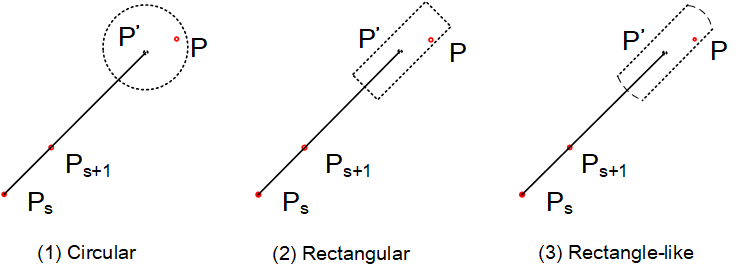
\includegraphics[scale=1.0]{Figures/Fig-Areas.png}\vspace{-1ex}
	%\caption{\small A trajectory is simplified by algorithm \dpa using distance metrics \ped, \sed and \dad, respectively.}
	\vspace{-1ex}
	\caption{\small Trajectory tracking in (1) a floating disc, (2) an infinite beam \cite{Chen:Space,Daescu:metric} and (3) a floating finite beam. Where $P_s$ is the start position of the sub-trajectory and $P'$ is the expected position of the moving object at time $P.t$ whose actually position at that time is $P$.}
	\vspace{-3ex}
	\label{fig:areas}
\end{figure}

\stitle{{Contributions}.}
To the end, we explore ways to track a moving object in a disc, an infinite beam and a finite beam, respectively, and design novel one-pass trajectory tracking algorithms that effectively and efficiently run for such areas. 

\ni (1) We develop a one-pass trajectory tracking algorithm \citt and theoretically prove that it has better effectiveness than \ldrh. Thus, we are able to effectively and efficiently track a moving object inside a floating disc (Section \ref{sec:circle}).
%\citt is more effective than \ldrh, great more efficient and a bit more effective than \grts (Section \ref{sec:circle}).

%\ni (2) We develop a one-pass trajectory tracking algorithm \sitt based on the intersection of sectors that tracks a moving object in a strip area. \sitt is the first algorithm that tracks a moving in a strip area, and is as concise and efficient as \citt (Section \ref{sec:strip}). %, and has a better compression ratio than \citt with a cost of a poorer accuracy.

\ni (2) We provide a convenient way to design new tracking shapes, \ie  an infinite and a finite beams, and develop novel one-pass trajectory tracking algorithms \sitt and \bitt such that we are able to effectively and efficiently track moving objects inside infinite and floating finite beams, respectively (Section \ref{sec:rectangle}). 
%\bitt is the first algorithm that tracks a moving object in a rectangle-like area, and it takes the advantages of both \citt and \sitt (Section \ref{sec:rectangle}). 
%\ie~\sitt based on the intersection of sectors that tracks a moving object in a strip area

\ni (3) Using three real-life trajectory datasets (Mopsi, SerCar, GeoLife), we finally conduct an extensive experimental study that compares our methods \citt and \bitt with representative trajectory tracking algorithms \ldrh (the first and the most efficient trajectory tracking algorithm) and \grts (the most effective trajectory tracking algorithm). The experimental results show that \citt and \bitt are both efficient and effective, and are feasible to track a moving object inside a disc and a beam, respectively (Section \ref{sec-exp}).


\eat{%%%%%%%%%%%%%%%%
\stitle{{Organization}}.
The remainder of the paper is organized as follows:
Section \ref{sec-pre} introduces the basic concepts and the \ldr and \ldrh approaches,
Sections \ref{sec:circle}, \ref{sec:strip} and \ref{sec:rectangle} present three one-pass algorithms that track in circular, strip and rectangle-like areas, respectively,
Section \ref{sec-exp} reports the experimental results of these methods, followed by related works in Section \ref{sec-related} and conclusion in Section \ref{sec-conclusion}.
All proofs are provided in the Appendix.
}%%%%%%%%%%%%%%%%eat



\section{Preliminary}	%\section{Overview of algorithms}
\label{sec-problem}


In this section, we introduce some basic concepts for trajectory simplification.
For convenience, notations used are summarized in \mytable{tab:notations}.

\stitle{Points}. A data point is defined as a triple $P(x, y, t)$, which represents that a moving object is located at {\em longitude} $x$ and {\em latitude} $y$ at {\em time} $t$. Note that these data points can be viewed as points in the x-y-t 3D Euclidean space.
%
%\textcolor{blue}{A data point could also be defined as a quadruple $P(x, y, z, t)$, where $z$ is {\em altitude}. However, to our knowledge, the current trajectory simplification algorithms all consider the x-y spatial information only, and the height information, if concerning, is treated as an independent dimension that could be simplified by piece-wise linear approximation methods \cite{Agarwal:Metric, ORourke:Fitting, Keogh:online, Luo:Streaming, Xie:Stream,Elmeleegy:Stream}.}


%We first introduce basic notations.
\stitle{Trajectory}. A \textit{trajectory} $\dddot{\mathcal{T}}\left[P_0, \ldots, P_n\right]$ is a sequence of points in a monotonically increasing order of their associated time values (\ie $P_i.t < P_j.t$ for any $0\le i<j\le n$). %Note that data points can be viewed as points in a three-dimension Euclidean space.
Intuitively, a trajectory is the path (or track) that a moving object follows through space as a function of time~\cite{physics-trajectory}.

\stitle{Directed line segment}. A directed line segment (or line segment for simplicity) $\mathcal{L}$ is defined as $\vv{P_{s}P_{e}}$, which represents the closed line segment that connects the start point $P_s$ and the end point $P_e$.
Note that here $P_s$ and $P_e$ are different points that may not in a trajectory $\dddot{\mathcal{T}}$.

%, and hence, we also use notation $\mathcal{R}$ instead of $\mathcal{L}$ when both $P_s$ and $P_e$ belong to $\dddot{\mathcal{T}}$.

For the projection of a directed line segment $\mathcal{L}$ on an \emph{x-y} 2D space, where $x$ and $y$ are the longitude and latitude, respectively, we also use $|\mathcal{L}|$ and $\mathcal{L}.\theta\in [0, 2\pi)$ to denote the length of $\mathcal{L}$ in the x-y 2D space, and its angle with the $x$-axis of the coordinate system $(x, y)$.  That is, the projection of a directed line segment $\mathcal{L}$ = $\vv{P_{s}P_{e}}$ on an \emph{x-y} 2D space is treated as a triple $(P_s, |\mathcal{L}|, \mathcal{L}.\theta)$.

%Intuitively, a trajectory can also be represented by a continuous $n$-pieces directed line segments (or line segment for simplicity) $\mathcal{L}_i$, $0\le i < n$, where  $\mathcal{L}_i = \vv{P_{i}P_{i+1}}$, represents the closed line segment that connects the start point $P_{i}$ and the end point $P_{i+1}$.

\stitle{Piece-wise line representation}. A \textit{piece-wise line representation} $\overline{\mathcal{T}}\left[\mathcal{L}_0, \ldots, \mathcal{L}_m\right]$ ($0< m \le n$) of a trajectory $\dddot{\mathcal{T}}\left[P_0, \ldots, P_n\right]$ is a sequence of continuous \textit{directed line segments} $\mathcal{L}_{i}$ = $\vv{P_{s_i}P_{e_i}}$ ($i\in\left[0,m\right]$) of $\dddot{\mathcal{T}}$ such that $\mathcal{L}_{0}.P_{s_0} = P_0$, $\mathcal{L}_{m}.P_{e_m} = P_n$ and  $\mathcal{L}_{i}.P_{e_i}$ = $\mathcal{L}_{i+1}.P_{s_{i+1}}$ for all $i\in\left[0, m-1\right]$.
Note that (1) each directed line segment in $\overline{\mathcal{T}}$ essentially represents a continuous sequence of data points in trajectory $\dddot{\mathcal{T}}$, (2) a piece-wise line representation is a simplified trajectory, \myblue{essentially the sequence of end points of all line segments}, {and (3) a point ($x$, $y$, $t$) on a spherical surface is  projected on a 2D flat plane in the piece-wise line representation.}


	\begin{table}
	\renewcommand{\arraystretch}{1.20}
	\vspace{-1ex}
	\caption{\small Summary of notations}
	\centering
	\footnotesize
	%\scriptsize
	\begin{tabular}{|c|l|}
		\hline
		{\bf Notations}& {\bf Semantics}   \\		\hline %\hline
		$P$ & a data point \\		\hline
		$\dddot{\mathcal{T}}$ & a trajectory $\dddot{\mathcal{T}}$ is a sequence of data points\\		\hline
		$\overline{\mathcal{T}}$&  {a piece-wise line representation of a trajectory $\dddot{\mathcal{T}}$}	\\		\hline
		$\mathcal{L}$ & a directed line segment  \\		\hline
		$\mathcal{M}$ & a distance metric of \ped, \sed or \dad \\		\hline
		$ped\left(P, \mathcal{L}\right)$ &  {the perpendicular Euclidean distance of point $P$ to line segment $\mathcal{L}$}	\\	\hline
		$sed\left(P, \mathcal{L}\right)$ & {the synchronous Euclidean distance of point $P$ to line segment $\mathcal{L}$} 	\\		\hline
		$dad\left(\mathcal{L}_1, \mathcal{L}_2\right)$ & {the direction-aware distance of line segment $\mathcal{L}_1$ to line segment $\mathcal{L}_2$} 	\\		\hline
		$\epsilon$ & an error bound \\		\hline
		$\mathcal{A}$ & a line simplification algorithm \\		\hline
		%\sector{} & a sector \\		\hline
		%		$\vv{A} \times \vv{B}$ & the cross product of (vectors) $\vv{A}$ and $\vv{B}$\\		\hline
		%		$\mathcal{H}(\mathcal{L})$ & The open half-plane to the left of $\mathcal{L}$ \\		\hline
		%		$\mathcal{R}$& a convex polygon \\		\hline
		%		$\mathcal{R}^*$ & the intersection of convex polygons \\		\hline
		%		$m$ & the maximum number of edges of a polygon\\		\hline
		%		$E^j$ & a group of edges labeled with $j$\\		\hline
		%		$g(e)$ & the label of an edge $e$ of polygons \\		\hline
		%		\circle{} & a synchronous circle\\		\hline
		%\cone{} & a spatio-temporal cone \\		\hline
		%		\pcircle{} & a cone projection circle \\		\hline
		%$\bigsqcap$ & intersection of geometries\\		\hline
		%$G$ &	the reachability graph of a trajectory\\		\hline
	\end{tabular}
	\label{tab:notations}
	\vspace{-1ex}
\end{table}


 For trajectory simplification, three distance metrics are commonly used, namely, the \emph{perpendicular Euclidean distance} (\ped), the \emph{synchronous Euclidean distance} \cite{Meratnia:Spatiotemporal} (\sed) and the \emph{direction-aware distance}\cite{Long:Direction, Zhang:Evaluation} (\dad).
%
Consider a data point $P$ and a directed line segment $\mathcal{L}$ = $\vv{P_{s}P_{e}}$.

\stitle{Perpendicular Euclidean distance}. The perpendicular Euclidean distance $ped\left(P, \mathcal{L}\right)$ of point $P$ to line segment $\mathcal{L}$ is $\min\{|PQ|\}$ for any point $Q$ on $\vv{P_{s}P_{e}}$.
%
\textcolor{blue}{This definition is also called the \emph{tolerance-zone} error measure \cite{Daescu:metric,Barequet:3D,Chen:Space,Imai:Optimal,Melkman:Optimal}.}
\textcolor{blue}{Note that in the field of computational geometry, (1) there is a slight variation of \emph{tolerance-zones}, called \emph{infinite beams} or \emph{parallel-strip} error measures \cite{Daescu:metric,Chen:Space}, which is the perpendicular Euclidean distance of a point to a line, and (2) it is believed that tolerance-zones could produce a compressed version that better captures the features of the original path/curve \cite{Daescu:metric,Barequet:3D,Chen:Space}. If not otherwise specified, we use tolerance-zones to evaluate algorithms.}
%, the most natural definition of \ped~\cite{Barequet:3D}	
	
\stitle{Synchronous Euclidean distance}. The synchronous Euclidean distance $sed\left(P, \mathcal{L}\right)$ of point $P$ to line segment $\mathcal{L}$ is $|\vv{PP'}|$ that is the Euclidean distance from $P$ to its \textit{synchronized data point} $P'$ \wrt $\mathcal{L}$, where the synchronized data point $P'$ \wrt $\mathcal{L}$ is defined as follows:
(a) $P'.x$ = $P_s.x +  c\cdot\left(P_e.x - P_s.x\right)$,
(b) $P'.y$ = $P_s.y +  c\cdot\left(P_e.y - P_s.y\right)$ and
(c) $P'.t$ = $P.t$, where $c= \frac{P.t-P_s.t}{P_e.t-P_s.t}$.

{Synchronized points are essentially virtual points with the assumption that an object moves along a straight line segment from $P_s$ to $P_e$ with a uniform speed, \ie the average speed $\frac{|\vv{P_sP_e}|}{P_e.t-P_s.t}$ between points $P_s$ and $P_e$ \cite{Cao:Spatio,Lin:Cised}. Then the \emph{synchronized point} $P'$ of a point $P$ \wrt the line segment $\vv{P_sP_e}$ is the expected position of the moving object on $\vv{P_sP_e}$ at time $P.t$, obtained by a linear interpolation \cite{Cao:Spatio}. More specifically, a synchronized point $P'_i$ of $P_i$ ($s\le i < e$) \wrt the line segment $\vv{P_sP_e}$ is a point on $\vv{P_sP_{e}}$ satisfying ${|\vv{P_sP'_i}|} = \frac{P_i.t - P_s.t}{P_e.t - P_s.t}\cdot {|\vv{P_sP_e}|}$, which means that the object moves from $P_s$ to $P_e$ at an average speed $\frac{|\vv{P_sP_e}|}{P_e.t-P_s.t}$, and its position at time $P_i.t$ is the point $P'_i$ on $\overrightarrow{P_sP_{e}}$ having a distance of $\frac{P_i.t - P_s.t}{P_e.t - P_s.t}\cdot|\vv{P_sP_e}|$ to $P_s$~\cite{Cao:Spatio, Lin:Cised,Meratnia:Spatiotemporal, Chen:Fast, Zhang:Evaluation}.}

\textcolor{blue}{Instead of directly using \sed,  \cite{Chen:Fast} introduces Local Integral Square \sed (\lissed, also called LSSD in \cite{Cao:Dots,Chen:Fast}) with $lissed(P_s,P_{s+k}) = \sum_{i=s}^{s+k-1} sed^2(P_i, \vv{P_sP_{s+k}})$. The most important feature of \lissed is that it can be computed in an incremental way, \ie given information about $lissed(P_s,P_{s+k})$, $lissed(P_s,P_{s+k+1})$ can be calculated in $O(1)$ time, such that algorithms using it (\eg~\bumr~\cite{Chen:Fast} and \dagots~\cite{Cao:Dots}) have lower time complexities compared with directly using \sed.
It is worth pointing out that (1) \lissed is  a special \sed-based \emph{error} measure rather than a new kind of \emph{distance} metric, (2) if the \lissed error bound of such an algorithm is set to $\epsilon^2$, then the maximal \sed error between the original and simplified trajectories is always not greater than $\epsilon$, and (3) the most recent algorithm directly using \sed, \ie~\cised, are very efficient, and has $O(n)$ time.}
%and (2) \lissed brings very different simplified trajectories compared with \sed
%\textcolor{blue}{Besides, in order to speed up the simplification, a few algorithms \cite{Chen:Fast, Wu:Graph,Cao:Dots} alternatively use an accumulation of square \sed, named Local Integral Square Synchronous Euclidean Distance (\lissed) \cite{Chen:Fast}, as the error bound. \bumr~\cite{Chen:Fast} is such a batch algorithm, and \dagots~\cite{Cao:Dots} follows the ideas of \cite{Chen:Fast} and provides an online version. These \lissed-equipped algorithms ensure that any \lissed from data points to their representing line segment is limited by a preset \lissed error bound.}


\stitle{Direction-aware distance}. The direction-aware distance $dad\left(\mathcal{L}_1, \mathcal{L}_2\right)$ is the direction deviation from $\mathcal{L}_1$ to $\mathcal{L}_2$, \ie $\Delta\left(\mathcal{L}_1.\theta, \mathcal{L}_2.\theta\right) = \min\{|\mathcal{L}_1.\theta - \mathcal{L}_2.\theta|, 2\pi - |\mathcal{L}_1.\theta - \mathcal{L}_2.\theta|\}$.
{Note \dad differs from \ped and \sed in that it is a measure of angle changes, rather than Euclidean distances, and the temporal information is also lost when using \dad.}





We illustrate these notations with examples.

\begin{example}
	\label{exm-notations}
	Consider {Figure}~\ref{fig:dp}, in which
	%
	(1) $\dddot{\mathcal{T}}\left[P_0, \ldots, P_{10}\right]$ is a trajectory having 11 data points,
	%
    (2) the set of two continuous line segments $\{\vv{P_0P_4}$, $\vv{P_4P_{10}}$\}, the set of four continuous line segments $\{\vv{P_0P_2}$, $\vv{P_2P_4}$, $\vv{P_4P_7}$, $\vv{P_7P_{10}}$\} and the set of three continuous line segments $\{\vv{P_0P_4}$, $\vv{P_4P_5}$, $\vv{P_5P_{10}}$\} are three piece-wise line representations of trajectory $\dddot{\mathcal{T}}$,
	%
	(3) $ped\left(P_4, \vv{P_0P_{10}}\right)=|\vv{P_4P^*_4}|$, where $P^*_4$ is the perpendicular point of $P_4$ \wrt line segment $\vv{P_0P_{10}}$,
	%
	(4) For $P_4$, its synchronized point $P'_4$ \wrt $\vv{P_0P_{10}}$ satisfies $\frac{|\vv{P_0P'_4}|}{|\vv{P_0P_{10}}|} = \frac{P_4.t - P_0.t}{P_{10}.t-P_0.t} = \frac{4-0}{10-0}= \frac{2}{5}$,
	%
	(5) $sed\left(P_4, \vv{P_0P_{10}}\right)= |\vv{P_4P'_4}|$, $sed\left(P_2, \vv{P_0P_{4}}\right)= |\vv{P_2P'_2}|$ and $sed\left(P_7, \vv{P_4P_{10}}\right)$ $=$ $|\vv{P_7P'_7}|$,
	where points $P'_4$, $P'_2$ and $P'_7$ are the synchronized points of $P_4$, $P_2$ and $P_7$ \wrt line segments $\vv{P_0P_{10}}$, $\vv{P_0P_{4}}$ and $\vv{P_4P_{10}}$, respectively.  and
    %
    (6) $dad\left(\vv{P_5P_6}, \vv{P_0P_{10}}\right)=\theta_{56}$ is the \dad of line segments $\vv{P_5P_6}$ to $\vv{P_0P_{10}}$.
\end{example}


\begin{figure}[tb!]
	\centering
	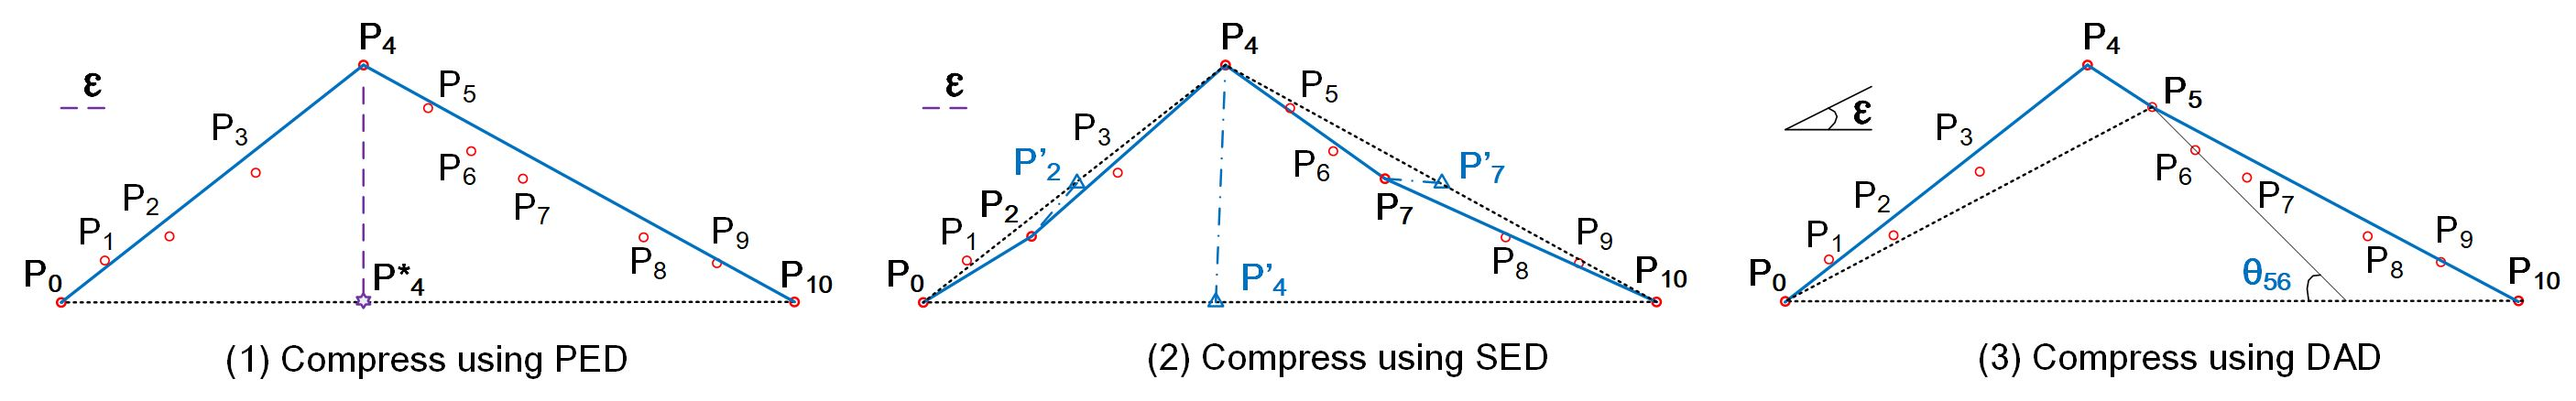
\includegraphics[scale=0.46]{Figures/Fig-DP.jpg}\vspace{-1ex}
	%\caption{\small A trajectory is simplified by algorithm \dpa using distance metrics \ped, \sed and \dad, respectively.}
	\caption{\small  A trajectory $\dddot{\mathcal{T}}[P_0, \ldots, P_{10}]$ with 11 points is compressed by the Douglas--Peucker algorithm \cite{Douglas:Peucker} using distance metrics \ped, \sed and \dad, respectively.}
		\vspace{-2ex}
	\label{fig:dp}
\end{figure}



%\stitle{Min-$\#$ problem}. Given a trajectory \trajec{T}$\left[P_0, \dots, P_n\right]$ and a pre-specified constant $\epsilon$, the \emph{min-$\#$} problem of trajectory simplification is to approximate the trajectory \trajec{T} with $\overline{\mathcal{T}}\left[\mathcal{L}_0, \ldots , \mathcal{L}_m\right]$ ($0< m \le n$), such that
%(1) on each of them the points $\left[P_{s_i}, \dots, P_{e_i}\right]$ are approximated by a line segment $\mathcal{L}_i = \vv{P_{s_i}P_{e_i}}$ with the maximum \ped or \sed \emph{error} of point $P_j$ (or \dad \emph{error} of line segment $|\vv{P_jP_{j+1}}|$) to line segment $\mathcal{L}_i$, $s_i \le j<e_i$,  less than $\epsilon$, and
%(2) $P_{s_i}$ and $P_{e_i} \in$ \trajec{T}.

%We finally introduce error bounded algorithms for trajectory simplification.

\stitle{\textcolor{blue}{Trajectory simplification algorithms}}. \myblue{Given a trajectory \trajec{T}$\left[P_0, \dots, P_n\right]$ and a pre-specified bound $\epsilon$, a \emph{trajectory simplification algorithm} $\mathcal{A}$ using \ped (respectively, \sed and \dad) produces a piece-wise line representation $\overline{\mathcal{T}}\left[\mathcal{L}_0, \ldots, \mathcal{L}_m\right]$ ($0< m \le n$) by applying distance checking of \ped (respectively, \sed and \dad) with respect to $\epsilon$, such that for each $i\in[0, m]$, line segment $\mathcal{L}_i = \vv{P'_{s_i}P'_{e_i}}$ ($s_i < e_i$) approximately represents the sub-trajectory \trajec{T}$_i\left[P_{s_i}, \dots, P_{e_i}\right]$ of \trajec{T}.}

\stitle{\textcolor{blue}{Error bounded algorithms}}. Given a trajectory \trajec{T}$\left[P_0, \dots, P_n\right]$ and a pre-specified bound $\epsilon$,
trajectory simplification algorithm $\mathcal{A}$ using \ped  (respectively, \sed and \dad) is \emph{error bounded} by $\epsilon$ if for each point $P_k$ ($k\in[0,n]$) in \trajec{T}, there exists a line segment $\mathcal{L}_i = \vv{P'_{s_i}P'_{e_i}}$ in $\overline{\mathcal{T}}$ with $s_i \le k \le e_i$ ($0\le i\le m$) such that the \ped distance $ped\left(P_k, \mathcal{L}_i\right)$  (respectively the \sed distance $sed\left(P_k, \mathcal{L}_i\right)$ and the \dad distance $dad\left(\vv{P_{k}P_{k+1}}, \mathcal{L}_i\right)$) is no more than  $\epsilon$.
%

Note that here \textcolor{blue}{there is no need} to require that for all $i\in[0,m]$, points $P'_{s_i}$ and $P'_{e_i}$ of $\overline{\mathcal{T}}$ belong to the original trajectory \trajec{T}. That is to say, \textcolor{blue}{data interpolations are allowed.}

\section{Compression Optimal Algorithms}
\label{sec-optimal}

This section reviews the compression optimal \lsa algorithms find the minimum number of points or segments to represent the original trajectory \wrt an error bound $\epsilon$.

The naive optimal algorithm (\opt) \cite{Imai:Optimal} first formulates the \emph{min-$\#$} problem as a graph reachability problem, and solves the problem in  $O(n^3)$ time, where $n$ is the number of the original points of a trajectory. It is initially designed to support \ped, but can easily be modified to support \sed and \dad.
By using \textit{convex hull} \cite{Toussaint:Optimal} and \textit{sector intersection} \cite{Melkman:Optimal}, faster optimal algorithms are proposed with an improved time complexity to $O(n^2 \log n)$. Further, \cite{Chan:Optimal} \textcolor{blue}{proves that the \emph{min-$\#$} problem (using \ped) for a general polygonal curve can be solved in $O(n^2)$ time by using the \textit{sector intersection} mechanism, and for some special curves (\eg a polygonal curve forming a part of a convex polygon), either open or closed (if there is an edge joining the first and the last points, then it is closed; otherwise, it is open), this problem can be solved in $O(n)$ time. Note that, in general, a trajectory is not necessary a convex or closed polygonal curve, instead, it is often open and concave. Thus, the best optimal algorithm for trajectory simplification using \ped still has $O(n^2)$ time.}
%
\textcolor{blue}{\optss~\cite{Chen:Fast} using \lissed also has a time complexity of $O(n^2)$, and}
%
algorithm \kw{SP} \cite{Long:Direction} is essentially an optimization of the original optimal algorithm using \dad that achieves $O(n^2)$ time.
%
However, all the above optimization mechanisms do not support \sed directly, and \opt remains the best optimal solution for \sed . {\em As all the optimized algorithms have the same effectiveness using the same distance metric, and essentially work for small size trajectories only, we choose algorithm \opt that supports \ped, \sed and \dad as the representative of optimal \lsa algorithms}.


%However, we argue that an optimal and a near optimal \lsa algorithms using \sed can achieve $O(n^2 \log n)$ time and $O(n^2)$ time, respectively, by applying the spatio-temporal cone intersection mechanism shown in Section~\ref{sec-cised} developed in our preview work \cised~\cite{Lin:Cised}.

%we introduce the naive optimal algorithm (\opt) \cite{Imai:Optimal} that runs in $O(n^3)$ time.
%The above optimized algorithms have the same effectiveness with the naive optimized algorithm using the same distance metric, thus, we won't go into them in detail.
%We then review a \ped specific optimal algorithm \optp \cite{Chan:Optimal} that achieves $O(n^2)$ time.
%Algorithms \opt and \optp are both evaluated in our experiments.
%Algorithm \opt is evaluated in our experiments.

%\subsection{The Naive Optimal Algorithm}
Given a trajectory \trajec{T}${[P_0, \ldots, P_n]}$ and an error bound $\epsilon$, algorithm \opt \cite{Imai:Optimal} solves the optimal trajectory simplification problem  in two steps: (1) it first constructs a reachability graph $G$ of \trajec{T}, and then (2) searches a shortest path from point $P_0$ to point $P_{n}$ in graph $G$.
%
The reachability graph of a trajectory \trajec{T}${[P_0, \ldots, P_n]}$ \wrt an error bound $\epsilon$ is $G$ = ($V$, $E)$, where (1) $V = \{P_0, \ldots, P_n\}$, and (2) for any nodes $P_s$ and $P_{s+k} \in V$ ($s\ge 0, k>0, s+k\le n$), edge $(P_s, P_{s+k}) \in E$ if and only if the distance of each point $P_{s+i} (0<i<k)$ to line segment $\vv{P_sP_{s+k}}$ is not greater than $\epsilon$.
%
Observe that in the graph $G$, (1) a path from nodes $P_0$ to $P_{n}$ is a representation of trajectory \trajec{T}. The path also reveals the subset of points of \trajec{T} used in the approximate trajectory, (2) the path length corresponds to the number of line segments in the approximate trajectory, and
(3) a shortest path is an optimal representation of trajectory \trajec{T}.

A straightforward way of constructing the reachability graph $G$ needs to check for all pairs of points $P_s$ and $P_{s+k}$ whether the distances of all points ($P_{s+i}$, $0<i<k$) to the line segment $\vv{P_sP_{s+k}}$ are less than $\epsilon$.
There are $O(n^2)$ pairs of points in the trajectory and checking the errors of all points $P_{s+i}$ to a line segment $\vv{P_sP_{s+k}}$ takes $O(n)$ time.
Thus, the construction step takes $O(n^3)$ time.
Finding a shortest path takes no more than $O(n^2)$ time. Hence, the straightforward algorithm, \ie~\opt, takes $O(n^3)$ time in total.
For space complexity, it needs $O(n^2)$ space.
%
Though the algorithm is initially developed using \ped, it is easy to see that it also supports \sed and \dad.


\begin{example}
	\label{exm-alg-optimal}
	Figure~\ref{fig:optimal} is an example of the \opt algorithm using \ped taking as input the trajectory \trajec{T} shown in Figure~\ref{fig:dp}. The reachability graph of \trajec{T} is constructed and a shortest path with 2 edges is founded.
	At last, the algorithm outputs two line segments $\vv{P_0P_4}$ and $\vv{P_4P_{10}}$.	
\end{example}
\vspace{-1ex}

\begin{figure}[tb!]
	\centering
	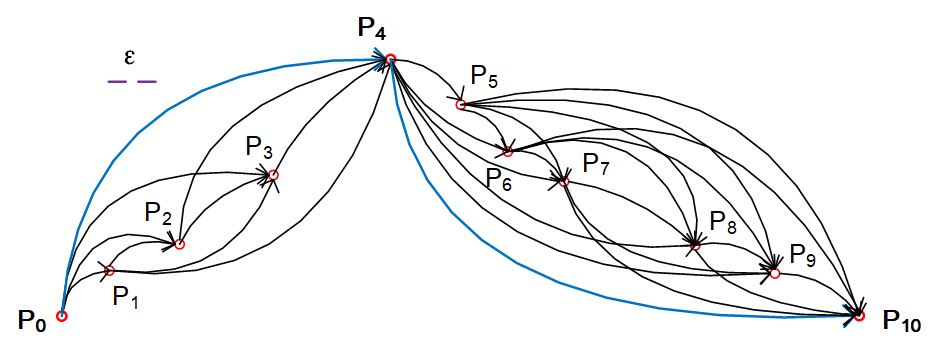
\includegraphics[scale=0.75]{Figures/Fig-Optimal.jpg}\vspace{-1ex}
	\caption{\small Example of reachability graph of trajectory \trajec{T}$[P_0, \ldots, P_n]$ whose shortest path is $(P_0, P_4, P_{10})$.}	\vspace{-3ex}
	\label{fig:optimal}
\end{figure}








\eat{%%%%%%%%%%%%%%%%%%%%%%%%20180722
\subsection{The Fast Optimal Algorithm Using \ped}
\label{subsec-optped}

Authors of \cite{Chan:Optimal} provide an optimal algorithm using \ped (\optp) that constructs the graph $G$ in $O(n^2)$ time, by using the \textit{sector intersection}\cite{Williams:Longest, Sklansky:Cone, Dunham:Cone, Zhao:Sleeve} mechanism.

For the start data point $P_s$, any point $P_{s+i}$ and $|\vv{P_sP_{s+i}}|>\epsilon$ ($i\in[1, k]$), there are two directed lines $\vv{P_sP^u_{s+i}}$ and $\vv{P_sP^l_{s+i}}$ such that $ped(P_{s+i}, \vv{P_sP^u_{s+i}})$ $=$ $ped(P_{s+i}, \vv{P_sP^l_{s+i}}) = \epsilon$ and either ($\vv{P_sP^l_{s+i}}.\theta < \vv{P_sP^u_{s+i}}.\theta ~and~\vv{P_sP^u_{s+i}}.\theta - \vv{P_sP^l_{s+i}}.\theta <\pi$) or ($\vv{P_sP^l_{s+i}}.\theta > \vv{P_sP^u_{s+i}}.\theta ~and~ \vv{P_sP^u_{s+i}}.\theta - \vv{P_sP^l_{s+i}}.\theta < -\pi)$. Indeed, they forms a \emph{sector} \sector{(P_s, P_{s+i}, \epsilon)} that takes $P_s$ as the center point and $\vv{P_sP^u_{s+i}}$ and $\vv{P_sP^l_{s+i}}$ as the border lines.


Then, given a point $P_s$, $0 \le s < n$, algorithm \optp builds a sector taking $P_s$ as the start point and checks for all points $P_{s+k}$, $k>0 ~and~ s+k \le n$, whether edge $(P_s, P_k)$ can be included in graph $G$. It can be added to the graph if and only if $(\bigsqcap_{i=1}^{k-1}\mathcal{S}(P_s, P_{s+i}, \epsilon)) \bigsqcap \vv{P_sP_{s+k}} \ne \{P_s\}$, \ie line segment $\vv{P_sP_{s+k}}$ ~passing through the common intersection area of sectors $\mathcal{S}(P_s, P_{s+i}, \epsilon))$, $0<i<k$.

There are $n$ points of $P_s$ in the trajectory and the checking of $(\bigsqcap_{i=1}^{k-1}\mathcal{S}(P_s, P_{s+i}, \epsilon)) \bigsqcap \vv{P_sP_{s+k}} \ne \{P_s\}$ for one $P_s$ takes $O(n)$ time.
Thus, the construction step takes $O(n^2)$ time and the algorithm takes $O(n^2)$ time in total.
For space complexity, this algorithm takes $O(n^2)$ space. However, it could be optimized to $O(n)$ space by the approach presented in \cite{Chen:Space}, whose fundamental idea is that it computes a shortest path in graph $G$ without having to maintain $G$ explicitly.

Algorithm \optp does not support \sed.


\begin{example}
	\label{exm-alg-optped}
	Figure~\ref{fig:optped} is a example of algorithm {\optp} taking as input the same trajectory $\dddot{\mathcal{T}}[P_0, \ldots, P_{10}]$. At the beginning, $P_0$ is the first start point, and points after $P_0$, \ie $P_1$, $P_2$, $P_3$, etc., each has a \emph{sector}. For example, the \emph{sector} $\mathcal{S}$($P_0$, $P_{2}$, $\epsilon$) takes $P_0$ as the center point and $\vv{P_0P^u_{2}}$ and $\vv{P_0P^l_{2}}$ as the border lines.
	Then, (1) for point $P_1$, edge $(P_0, P_1)$ is sure added to the graph $G$;
	(2) for point $P_2$, because $\bigsqcap_{i=1}^{2}\mathcal{S}(P_0, P_{0+i}, \epsilon) \ne \{P_0\}$ and $P_2$ is in the intersection area, edge $(P_0, P_2)$ is added to the graph $G$;
	(3) for points $P_3$ and $P_4$, edges $(P_0, P_3)$ and $(P_0, P_4)$ are added to the graph $G$ in turn;
	(4) for point $P_5$, because $P_5$ is NOT in the intersection area, edge $(P_0, P_5)$ should not be added to the graph $G$.
	After all edges start from $P_0$ have been checked, the process goes to the next step that takes $P_1$ as the new start point, and the process repeats.
	At last, the algorithm builds the same graph $G$ as shown in Figure~\ref{fig:optimal}, and outputs two line segments $\vv{P_0P_4}$ and $\vv{P_4P_{10}}$.
\end{example}

\begin{figure}[tb!]
	\centering
	\hspace{-1ex}\includegraphics[scale=0.66]{Figures/Fig-OptPed.jpg}\vspace{-3ex}
	\caption{\small The trajectory $\dddot{\mathcal{T}}$ is compressed by the fast optimal algorithm using \ped to two line segments.}	\vspace{-3ex}
	\label{fig:optped}
\end{figure}

}

\eat{%%%%%%%%%%%%%%%%%%%%%%%%%%%%%%%%%%%%%%%
\subsection{The Optimal Algorithm using \sed}
The constructing of the reachability graph $G$ using \sed can be optimized, by using the \textit{spatio-temporal cone intersection} mechanism (See Section~\ref{sec-siped}).

Given a point $P_s$, $0 \le s < n$, the optimal builds a cone taking $P_s$ as the start point and checks for all points $P_{s+k}$, $k>0 ~and~ s+k \le n$, whether $(P_s, P_k)$ can be included in graph $G$ by checking $(\bigsqcap_{i=1}^{k-1}\mathcal{C}(P_s, P_{s+i}, \epsilon)) \bigsqcap \vv{P_sP_{s+k}} \ne \{P_s\}$, \ie line segment $\vv{P_sP_{s+k}}$ ~passing through the common intersection area of cones $\mathcal{C}(P_s, P_{s+i}, \epsilon))$, $0<i<k$.

The checking of intersection of cones is equal to check the intersection of circles on a plane \cite{Lin:Cised}, which is claimed of $O(n \log n)$ time for $n$ circles~\cite{Shamos:Circle}.
There are $n$ points of $P_s$ in the trajectory and the checking for one $P_s$ takes $O(n \log n)$ time.
Thus, the construction step takes $O(n^2 \log n)$ time and the algorithm takes $O(n^2 \log n)$ time in total.

\stitle{Remark}.
If we approximate each circle by its $m$-edges inscribed regular polygon and approximate the intersection of $n$ circles on a plane by the intersection of their inscribed regular polygons, the way \cised does, then we get a near optimal graph $G'$ such that $\lim_{m \to \infty}{G'=G}$, and a \textit{near optimal} algorithm using \sed, \ie ~\nopts, that achieves $O(n^2)$ time. The space complexity of the near optimal algorithm also achieves $O(n)$ by combining the approach of \cite{Chen:Space}.
}


%%%%%%%%%%%%%%%%%%%%%%%%%%%%%%%%%%%%%%%%%%%%%%%%%%%%%%%%%%%%%%%%%%%%%%%%
%\vspace{-1ex}
\section{Compression Sub-Optimal Algorithms}
\label{sec-subopt}
%%%%%%%%%%%%%%%%%%%%%%%%%%%%%%%%%%%%%%%%%%%%%%%%%%%%%%%%%%%%%%%%%%%%%%%%

%In particular, the state-of-the-art the sub-optimal line simplification approaches can be classified into three categories.


This section reviews compression sub-optimal algorithms solving the \emph{min-$\#$} problem of trajectory simplification, as shown in the taxonomy of Section~\ref{sec-intro}.

\subsection{Batch Algorithms}
Batch algorithms essentially apply global distance checking policies for trajectory simplification, and can be either top-down or bottom-up.
Global checking policies enforce batch algorithms to have an entire trajectory first \cite{Meratnia:Spatiotemporal}.

(1) Top-down algorithms recursively divide a trajectory into sub-trajectories until the stopping condition is met.
Algorithms Ramer \cite{Ramer:Split} and Douglas-Peucker (\dpa)  \cite{Douglas:Peucker} are similar, and support all the three distances \ped, \sed and \dad. \myblue{Note that the \dpa using \sed is also called TD-TR \cite{Meratnia:Spatiotemporal}}.
An improved method of \dpa with a time complexity of $O(n\log n)$, based on \emph{convex hulls}, is proposed in \cite{Hershberger:Speeding}, which is the best \dpa based  algorithm in terms of time complexities, and is designed for \ped only, not for \sed and \dad.

%Variations on the Top-Down algorithm were independently introduced in several fields in the early 1970's. Douglas-Peucker algorithm [9] in cartography and Ramer  algorithm [29] in image processing share the similar routine, and they support all the three ...


(2) Bottom-up algorithms are the natural complement of top-down ones, and they recursively merge adjacent sub-trajectories with the smallest distance, initially $n/2$  sub-trajectories for a trajectory with $n$ points, until the stopping condition is met. In each iteration, the distances of newly generated line segments are recalculated.
To our knowledge, Theo-Pavlidis (\tpa) \cite{Pavlidis:Segment} is the only bottom-up batch \lsa algorithm that supports \ped, \sed and \dad. \textcolor{blue}{Besides, \bumr~\cite{Chen:Fast} using \lissed is also a bottom-up algorithm.}

Note that, compared with top-down algorithms, bottom-up algorithms fit better for trajectories with lower sampling rates, as they typically need more rounds to merge smaller line segments into larger line segments. {\em Batch algorithms basically work for small and medium size trajectories, and we choose \myblue{the famous top-down algorithm} \dpa and \myblue{the classic bottom-up algorithm} \tpa that all support \ped, \sed and \dad  as the representatives of batch \lsa algorithms}.


%We next review algorithms Douglas-Peucker and Theo Pavlidis evaluated in out experiments.




%%%%%%%%%%%%%%%%%%%%%%%%%%%%%%%%%%%%%%%%%%%%%%%%%%%%%%
%\vspace{-1ex}
%\subsubsection{Douglas-Peucker Algorithm}

\eat{
%%%%%%%%%%%%%%%%%%%%%Baseline Algorithm
\begin{figure}[tb!]
	%\vspace{-2ex}
	\vspace{1ex}
	\begin{center}
		{\small
			\begin{minipage}{3.3in}
				\myhrule \vspace{-1ex}
				\mat{0ex}{
					{\bf Algorithm}~$\dpa(\dddot{\mathcal{T}}[P_0,\ldots,P_n], \epsilon)$\\
					\sstab
					\bcc \hspace{1ex}\=\For each point $P_i$ ($i\in[0,n]$) in $\dddot{\mathcal{T}}[P_0, \ldots, P_n]$ \Do\\
					\icc \>\hspace{3ex}compute $ped(P_i, {\mathcal{L}})$ between $P_i$ and ${\mathcal{L}}(P_0, P_n)$;\\
					\icc \> \Let $ped(P_k, {\mathcal{L}})$ := $\max \{ped(P_0, {\mathcal{L}}), \ldots, ped(P_n, {\mathcal{L}}) \}$;\\
					\icc \> \If $ped(P_k, {\mathcal{L}}) \le\epsilon$ \Then \\
					\icc \> \hspace{3ex}\Return $\{\mathcal{L}(P_0,P_n)\}$.\\
					\icc \> \Else\\
					\icc \> \hspace{3ex}\Return $\dpa($\trajec{T}$[P_0, \ldots, P_k], \epsilon)\cup\dpa($\trajec{T}$[P_{k}, \ldots, P_n], \epsilon)$.
				}
				\vspace{-2.5ex}
				\myhrule
			\end{minipage}
		}
	\end{center}
	\vspace{-3ex}
	\caption{\small Basic Douglas-Peucker algorithm}
	\label{alg:dp}
	\vspace{-3ex}
\end{figure}
}
%%%%%%%%%%%%%%%%%%%%%%%%%%%%%%%%%%%%%


\subsubsection{Algorithm Douglas-Peucker  (\dpa) \cite{Douglas:Peucker}}
It is invented for reducing the number of points required to represent a digitized line or its caricature in the context of computer graphics and image processing.
{Originally, it uses \ped, however, it can be easily extended to support \sed and \dad.}


Given a trajectory $\dddot{\mathcal{T}}[P_0, \ldots, P_n]$ and an error bound $\epsilon$,  algorithm \dpa uses the first point $P_0$ and the last point $P_n$ of \trajec{T} as the start point $P_s$ and the end point $P_e$ of the first line segment $\mathcal{L}(P_0, P_n)$, then it calculates the distance $ped(P_i, {\mathcal{L}})$ for each point $P_i$ ($i\in[0,n]$). If $ped(P_k, {\mathcal{L}})$ = $\max \{ped(P_0, {\mathcal{L}}), \ldots, ped(P_n, {\mathcal{L}}) \} \le \epsilon$, then it returns $\{\mathcal{L}(P_0,P_n)\}$. Otherwise, it divides \trajec{T} into two sub-trajectories \trajec{T}$[P_0, \ldots, P_k]$ and \trajec{T}$[P_{k}, \ldots, P_n]$, and recursively compresses these sub-trajectories until the entire trajectory has been considered.
%
The time complexity of \dpa is $\Omega(n)$ in the best case, but is $O(n^2)$ in the worst case.

%The basic \dpa uses \ped, however, it also supports \sed \cite{Meratnia:Spatiotemporal} that runs in the same routine as using \ped. %, except that $ped$ in
%Figure~\ref{alg:dp} is replace by $sed$.



\begin{example}
	\label{exm-alg-lsa}
	Consider the trajectory $\dddot{\mathcal{T}}[P_0,\ldots,P_{10}]$ shown in Figure~\ref{fig:dp}.
	The $\dpa$ Algorithm firstly creates $\vv{P_0P_{10}}$, then it calculates the distance of each point in $\{P_0,\ldots,P_{10}\}$ to $\vv{P_0P_{10}}$.
	It finds that $P_{4}$ has the maximum distance to $\vv{P_0P_{10}}$, which is greater than $\epsilon$. Then it goes to compress sub-trajectories $[P_0, \ldots, P_{4}]$ and $[P_{4}, \ldots, P_{10}]$, separately.
	When using \sed (right), the sub-trajectory $[P_4,\ldots, P_{10}]$ is further split to $[P_4$, $\ldots$, $P_7]$ and $[P_7$, $P_{10}]$.
	Finally, the algorithm outputs two continuous directed line segments $\vv{P_0P_4}$ and $\vv{P_4P_{10}}$ when using \ped, and three continuous directed line segments $\vv{P_0P_4}$, $\vv{P_4P_7}$ and $\vv{P_7P_{10}}$ when using \sed.
\end{example}




\subsubsection{Algorithm Theo-Pavlidis  (\tpa) ~\cite{Pavlidis:Segment}}
It originally employs the global checking policy to output disjoint line segments, and we slightly modify it to have continuous line segments.

Given a trajectory $\dddot{\mathcal{T}}[P_0, \ldots, P_n]$ and an error bound $\epsilon$,
algorithm \tpa begins by creating the finest possible  trajectory approximation: $[P_0, P_1]$, $[P_1, P_2], \ldots,[P_{n-1}, P_n]$, so that $n$ segments are used to approximate the original trajectory.
Next, for each pair of adjacent segments $[P_{s}, P_{s+j}]$ and $[P_{s+j}, P_{s+k}]$ ($0\le s<s+j < s+k \le n$),
the  distance $ped(P_{s+i}, \vv{P_sP_{s+k}})$ of each point $P_{s+i}$ ($0<i<k$) to the line segment $\vv{P_sP_{s+k}}$, is calculated, and the max distance is saved and denoted as the \emph{cost} of merging them.
Then \tpa begins to iteratively merge the adjacent segment pair with the lowest cost
until no cost is below $\epsilon$.
After the pair of adjacent segments $[P_{s}, P_{s+j}]$ and $[P_{s+j}, P_{s+k}]$ are merged to a new segment $[P_{s}, P_{s+k}]$, \tpa needs to recalculate the costs of the new segment with its preceding and successive segments, respectively.
%
Algorithm \tpa runs in $O(n^2/K)$ time, where $K$ is the number of the final segments.
Similar to the \dpa algorithm, the \tpa algorithm originally supports \ped, and it can be easily extended to support \sed and \dad as well.

\begin{figure}[tb!]
	\centering
	\includegraphics[scale=0.425]{Figures/Fig-pavlidis.jpg}\vspace{-1ex}
	\caption{\small The trajectory $\dddot{\mathcal{T}}[P_0, \ldots, P_{10}]$ is compressed by the \pavlidis~algorithm using \ped to two line segments. The triple $(i, j, cost)$ is the $cost$ of merging the line segments $\overline{P_iP_t}$ and $\overline{P_tP_j}$.}	\vspace{-2ex}
	\label{fig:pavlidis}
\end{figure}

\begin{example}
	\label{exm-alg-pavlidis}
	Figure~\ref{fig:pavlidis} is an example of the \tpa algorithm.
	
	\ni (1) Initially, $10$ line segments are created, and for each pair of adjacent segments, the costs of merging them are calculated and saved. For example, the cost of merging $\vv{P_0P_1}$ and $\vv{P_1P_2}$ is $ped(P_{1}, \vv{P_0P_{2}}) = 0.32\epsilon$.
	%
	(2) The cost of merging $\vv{P_6P_7}$ and $\vv{P_7P_8}$ is $0.02\epsilon$, which is the minimal value among all costs. Hence, $\vv{P_6P_7}$ and $\vv{P_7P_8}$ are merged to $\vv{P_6P_8}$. The cost of merging $\vv{P_5P_6}$ and $\vv{P_6P_8}$, and the cost of merging $\vv{P_6P_8}$ and $\vv{P_8P_9}$ are further updated to $0.37\epsilon$ and $0.11\epsilon$, respectively.
	%
	(3) $\vv{P_6P_8}$ and $\vv{P_8P_9}$ are merged to $\vv{P_6P_9}$. The cost merging $\vv{P_5P_6}$ and $\vv{P_6P_9}$, and the cost of merging $\vv{P_6P_9}$ and $\vv{P_9P_{10}}$ are also updated.
	%
	(4) At last, the algorithm outputs two line segments $\vv{P_0P_4}$ and $\vv{P_4P_{10}}$.
\end{example}




\subsection{Online Algorithms}

Online \lsa algorithms adopt local checking policies by restricting the distance checking within a sliding or opening window such that there is no need to have the entire trajectory ready before compressing. That is, online algorithms essentially combine {\em batch algorithms} with {\em sliding or opening windows}, \eg\
\opwa \cite{Meratnia:Spatiotemporal} is a combination of top-down algorithm \dpa and opening windows while \kw{SWAB} \cite{Keogh:online} is a combination of bottom-up algorithm \tpa and \textit{sliding windows}.
%
Though these algorithms support the three distance metrics \ped, \sed and \dad, they still have high time and/or space complexities \cite{Liu:BQS}.
%
\textcolor{blue}{Besides, in environments like wireless sensor networks, online algorithms also need to address the problem of balancing the trade-off between the energy cost due to communication and the accuracy of the trajectories' detection and representation \cite{Ghica:DTracking}, and controlling the ``freshness'' (i.e., the latency) of the simplified data by a careful management of the data buffer of an online algorithm \cite{Ghica:DTracking}.}
%
To design more efficient online algorithms, techniques typically need to be designed closely coupled with distance metrics.
Indeed, \bqsa \cite{Liu:BQS} and \squishe \cite{Muckell:Compression} propose to utilize convex hulls and priority queues, respectively, and they speed up trajectory simplification using \ped and \sed, respectively.
\textcolor{blue}{\dagots~\cite{Cao:Dots} is an online method using \lissed that could be computed in an incremental way.}
To our knowledge, no specific techniques have been developed for \dad.
Hence, {\em we choose algorithms \bqsa (\myblue{the performance optimized online algorithm, specific for \ped}), \squishe (\myblue{the famous online algorithm, specific for \sed}), \textcolor{blue}{\dagots (\myblue{using \lissed and recommended in the recent evaluation work \cite{Zhang:Evaluation}})} and \opwa (\myblue{a well-known online algorithm based on \dpa that is compatible with \dad}) as the representatives of online algorithms using \ped, \sed, \textcolor{blue}{\lissed} and \dad, respectively}.



\subsubsection{Algorithm \opwa \cite{Meratnia:Spatiotemporal}.}
It combines the top-down and opening window strategies, and enforces the constrained global checking in the window. Like \dpa, it supports \ped, \sed and \dad.

Given a trajectory $\dddot{\mathcal{T}}[P_0, \ldots, P_n]$ and an error bound $\epsilon$, algorithm \opwa~\cite{Meratnia:Spatiotemporal} maintains a window $W[P_s, \ldots, P_k]$, where $P_s$ and $P_k$ are the start and end points, respectively. Initially, $P_s$ = $P_0$ and $P_k$ = $P_1$, and the window $W$ is gradually expanded by adding new points one by one. \opwa tries to compress all points in $W[P_s, \ldots, P_k]$ to a single line segment $\mathcal{L}(P_{s}, P_{k})$. If the distances $ped(P_i, {\mathcal{L}})\le \epsilon$ for all points $P_i$ ($i\in[s, k]$), it simply expands $W$ to $[P_s, \ldots, P_k, P_{k+1}]$ $(k+1\le n)$ by adding a new point $P_{k+1}$. Otherwise, it produces a new line segment $\mathcal{L}(P_{s}, P_{k-1})$, and replaces $W$ with a new window $[P_{k-1},\ldots,P_{k+1}]$.  The above process repeats until all points in $\dddot{\mathcal{T}}$ have been considered. The process is similar for \sed and \dad.
%
%\textcolor[rgb]{0.00,0.07,1.00}{According to the different methods of selecting the end points of a line segment, Open Window can further be divided into Normal Penning Window and Before Opening Window~\cite{Meratnia:Spatiotemporal}. When the distance of the point to compressed trajectory exceeds a certain threshold, Normal Opening Window algorithm select that point as the end point, while Before Opening Window select the last point within the window as the end point of the current trajectory.}
%
The time complexity of algorithm \opwa remains in $O(n^2)$ time, the same as the \dpa algorithm.


\subsubsection{Algorithm BQS Using \ped \cite{Liu:BQS}}
It is essentially an efficiency optimized \opwa algorithm \cite{Meratnia:Spatiotemporal}, and reduces the running time by introducing convex hulls to pick out a certain number of points, which makes it dedicated for \ped.

For a buffer $W$ with sub-trajectory $[P_s, \ldots, P_k]$, it splits the space into four quadrants. A buffer here is similar to a window in \opwa \cite{Meratnia:Spatiotemporal}. For each quadrant, a rectangular bounding box is firstly created using the least and highest $x$ and $y$ values among points $\{P_s,\ldots,P_k\}$, respectively. Then another two bounding lines connecting points $P_s$ and $P_{h}$ and points $P_s$ and $P_{l}$ are created such that lines $\vv{P_sP_{h}}$ and $\vv{P_sP_{l}}$ have the largest and smallest angles with the $x$-axis, respectively.
Here $P_{h},P_{l} \in\{P_s,\ldots,P_k\}$. The bounding box and the two lines together form a convex hull.
Each time a new point $P_k$ is added to buffer $W$, \bqsa first picks out at most eight significant points from the convex hull in a quadrant. It calculates the distances of the significant points to line $\vv{P_sP_k}$, among which the largest distance $d_{u}$ and the smallest distance $d_l$ are an upper bound and  a lower bound of the distances of all points in $[P_s, \ldots, P_k]$ to line $\vv{P_sP_k}$.
(1) If $d_l\ge \epsilon$, it produces a new line segment $\mathcal{L}(P_{s}, P_{k-1})$, and produces a new window $[P_{k-1},\ldots,P_{k}]$ to replace $W$.
(2) If $d_u < \epsilon$, it simply expands buffer $W$ to $[P_s, \ldots, P_k, P_{k+1}]$ $(k+1\le n)$ by adding a new point $P_{k+1}$.
(3) Otherwise, it computes all distances $d(P_i, {\mathcal{L}(P_s,P_k)})$ ($i\in[s, k]$) as algorithm \dpa does.
%
The time complexity of \bqsa remains $O(n^2)$. However, its simplified version \fbqsa has a linear time complexity by essentially avoiding case (3) to speed up the process.


\begin{figure}[tb!]
	%\vspace{-1ex}
	\centering
	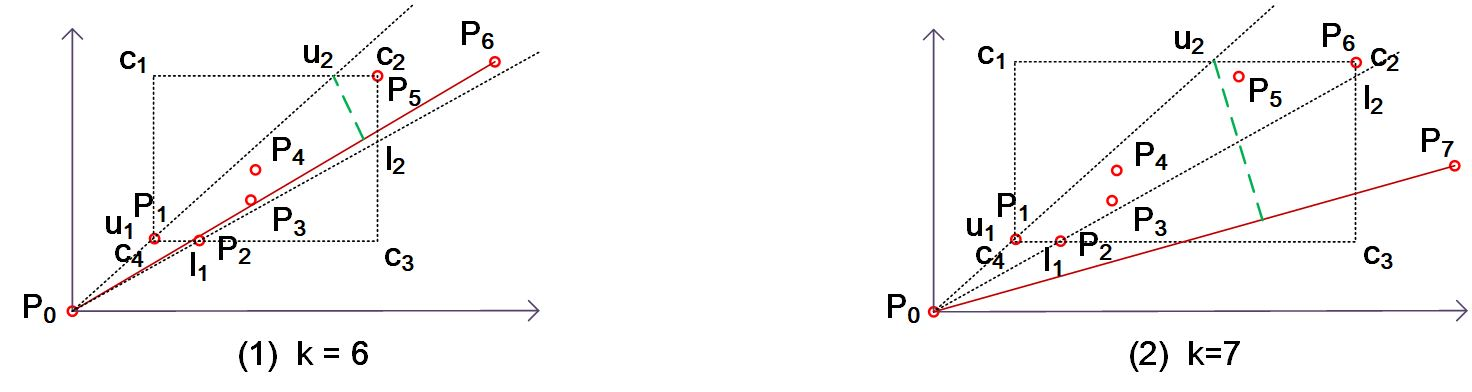
\includegraphics[scale = 0.66]{Figures/Fig-BQS.jpg}
	\vspace{-1ex}
	\caption{{\small Examples for algorithm \bqsa.}}
	\label{fig:bqs}
	\vspace{-2ex}
\end{figure}


\begin{example}
	\label{exm-alg-bqs}
	Figure~\ref{fig:bqs} is an example of \bqsa. The bounding box $c_1c_2c_3c_4$ and the two lines $\vv{P_sP_{h}} = \vv{P_0P_1}$ and $\vv{P_sP_{l}} = \vv{P_0P_2}$ form a convex hull $u_1u_2c_2l_2l_1c_4$. \bqsa computes the distances of $u_1,u_2,c_2,l_2,l_1$ and $c_4$ to line $\vv{P_0P_6}$ when $k=6$ or to line $\vv{P_0P_7}$ when $k=7$.
	%
	When $k=6$, all these distances to $\vv{P_0P_6}$  are less than $\epsilon$, hence \bqsa goes on to the next point (case 2); When $k=7$,
	the max and min distances to $\vv{P_0P_7}$ are larger and less than $\epsilon$, respectively, and \bqsa needs to compress sub-trajectory $[P_0, \ldots, P_7]$ along the same line as \dpa (case 3).
\end{example}




\subsubsection{Algorithm SQUISH-E Using \sed~\cite{Muckell:Compression}}
It is an online bottom-up algorithm that is {dedicated for \sed}, and has two forms: \squishe($\lambda$) ensuring the compression ratio $\lambda$, and \squishe($\epsilon$) ensuring the \sed error bound $\epsilon$. Here we adopt \squishe($\epsilon$), as we focus on error bounded trajectory simplification.

\eat{%%%%%%%%%%%%%%%%
taking as input a trajectory \trajec{T} and two additional parameters $\lambda$ and $\epsilon$.
It first compresses trajectory \trajec{T} while striving to minimize \sed error and achieving the compression ratio of $\lambda$. Then, it further compresses \trajec{T} as long as this compression will not increase the max \sed error beyond $\epsilon$.

Meanwhile, \squishe($\lambda$) is the case where $\epsilon$ is set to $0$ and therefore it minimizes \sed error ensuring the compression ratio of $\lambda$, and
\squishe($\epsilon$) denotes another case, \ie the \emph{min-$\#$ problem}, where $\lambda$ is set to $1$ and therefore it maximizes compression ratio while keeping \sed error under $\epsilon$.
In this paper, we only discuss \squishe($\epsilon$).
}%%%%%%%%%%%%%%%%%%%%

Algorithm \squishe optimizes algorithm \tpa with a doubly linked list $Q$. Each node in the list is a tuple $P(pre, suc, mnprio, prio )$, where $P$ is a trajectory data point, $pre$ and $suc$ are the predecessive  and successive points of $P$, respectively,  $prio$ is the priority of $P$ defined as an upper bound of the \sed error that the removal of $P$ introduces, and $mnprio$ is the max priority of its predecessive and successive points removed from the list.
%
Initially, trajectory points are loaded to $Q$ one by one.
At the same time, $mnprio$ of each point is set to $zero$ as no node has been removed from the list.
Moreover, the priorities of points $P_0$ and $P_{|Q|-1}$ are set to $\infty$, and the priority of point $P_i$ ($0<i<|Q|-1$) is set to $sed(P_i, \vv{pre(P_{i})suc(P_{i})})$.
%
Then, \squishe finds and removes a point $P_j$ from $Q$ that has the lowest priority $prio(P_j)<\epsilon$, and the properties $mnprio$ of predecessor $pre(P_j)$ and successor $suc(P_j)$ are updated to $\max(mnprio(pre(P_j)), prio(P_j))$ and $\max(mnprio(suc(P_j)), prio(P_j))$, respectively.
Next, the properties $prio$ of $pre(P_j)$ and $suc(P_j)$ are further updated to $mnprio(pre(P_j))$ + $sed(pre(P_j), \vv{pre(pre(P_{j}))suc(P_{j})})$ and $mnprio(suc(P_j))$ + $sed(suc(P_j),\vv{pre(P_{j})suc(suc(P_{j}))})$, respectively.
%
After that, a new point is read to the list and the information of its predecessor in the list is updated.
%
The above process repeated until that no points have a priority smaller than $\epsilon$.
%
\squishe finds and removes a point from $Q$ that has the lowest priority in $O(\log |Q|)$ time, where $|Q|$ denotes the number of points stored in $Q$.
Thus, \squishe runs in $O(n\log |Q|)$ time and $O(|Q|)$ space.



\begin{figure*}[tb!]
	\centering
	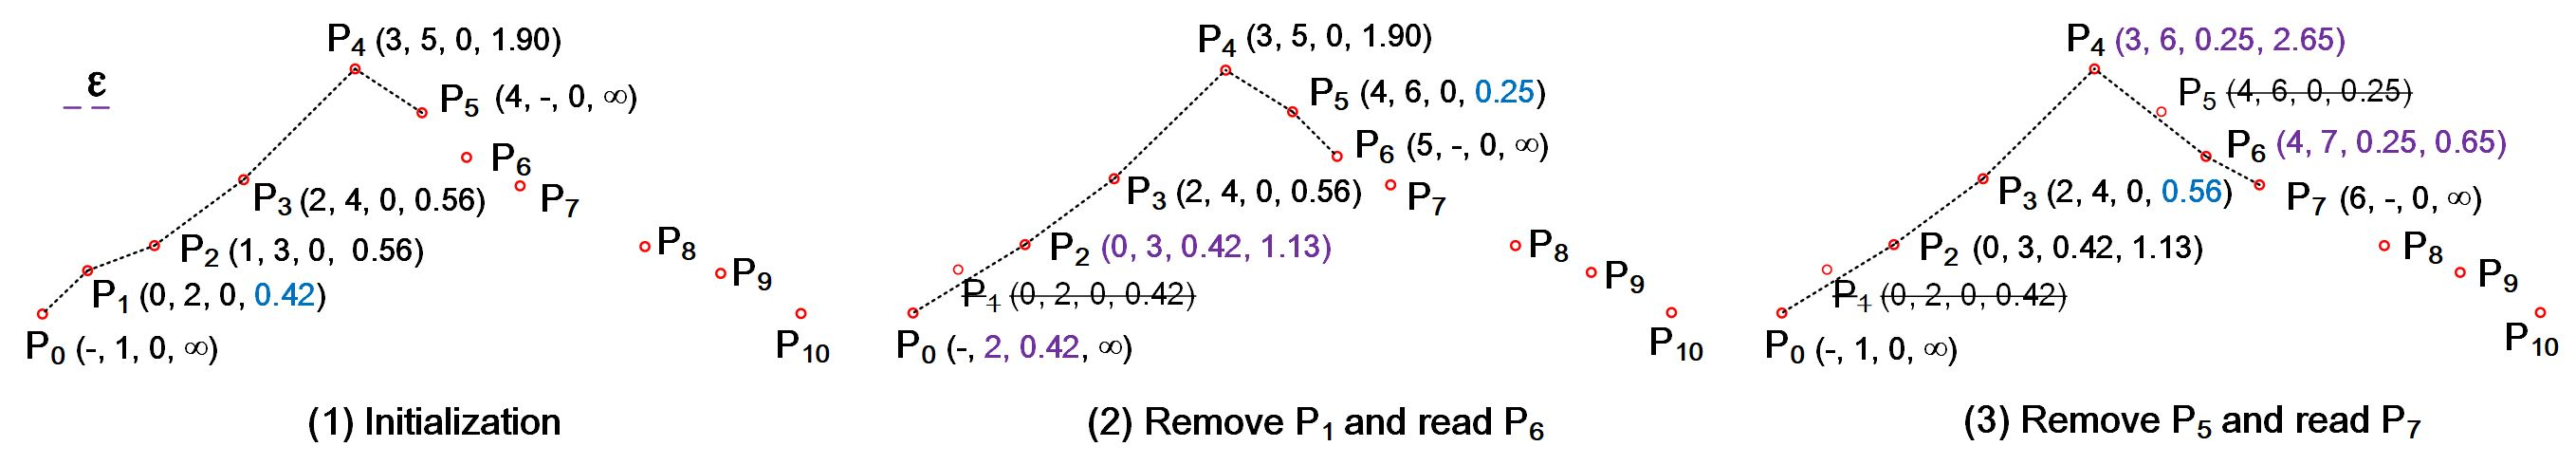
\includegraphics[scale=0.48]{Figures/Fig-Squishe.jpg}
	\vspace{-2ex}
	\caption{\small The trajectory $\dddot{\mathcal{T}}[P_0, \ldots, P_{10}]$ is compressed by the \squishe algorithm using \sed to five line segments. The size of Q is 6, and the data structure after point $P$ is a tuple $(pre, suc, mmprio, prio)$. }
	\vspace{-1ex}
	\label{fig:squishe}
\end{figure*}



\begin{example}
	\label{exm-alg-squishe}
	Figure~\ref{fig:squishe} is an example of \squishe.
	%
	(1) Initially, $|Q| = 6$ points are read to the list. The tuple $(pre, suc, mmprio, prio)$ for each point is initialized. For example, the tuple of $P_1$ is set to $(0, 2, 0, 0.42\epsilon)$, where $0.42\epsilon$ is the \sed from $P_1$ to $\vv{P_0P_2}$.
	%
	(2) The priority of $P_1$ has the minimal value, thus, it is removed from the list.
	The $mnprio$ properties of $P_0$ and $P_2$ are updated to $max\{mnprio(pre(P_1)), prio(P_1)\}$ = $max\{mnprio(P_0), prio(P_1)\}$ = $max\{0, 0.42\epsilon\}$ = $0.42\epsilon$, and $max\{mnprio(P_2), ~prio(P_1)\}$ = $0.42\epsilon$, respectively.
	Furthermore, the $prio$ property of $P_2$ is updated to $mnprio(suc(P_j)) + sed(suc(P_j),\vv{pre(P_{j})suc(suc(P_{j}))})$ = $mnprio(P_2) + sed(P_2,\vv{P_0P_3})$ = $0.42\epsilon + 0.71\epsilon$ = $1.13\epsilon$, and the $prio$ property of $P_0$ is still $\infty$.
	Then, $P_6$ is read, and the information of $P_5$ is updated.
	%
	(3) $P_5$ is removed and $P_7$ is read to the list.
	%
	(4) {Finally, the algorithm outputs 5 line segments $\vv{P_0P_2},\vv{P_2P_4},\vv{P_4P_7},\vv{P_7P_9}$ and $\vv{P_9P_{10}}$}.
\end{example}

\subsubsection{\textcolor{blue}{Algorithm DOTS Using \lissed~\cite{Cao:Dots}}}
\textcolor{blue}{It is a directed acyclic graph based online trajectory simplification method that supports \lissed. Other than the optimal and near optimal algorithms \cite{Chen:Fast,Daescu:metric} that find a shortest path after completely constructing the reachability graph, \dagots~incrementally determines the shortest path when constructing the reachability graph \cite{Cao:Dots}.}
%, \ie it runs in a recursive manner.
%before the whole graph is completely constructed,

\textcolor{blue}{Algorithm \dagots first shows that the reachability graph of an input trajectory retrogrades to a tree structure. It also observes that the local approximation error $lissed(P_s,P_{s+k})$ is growing with respect to $k$, thus, it is reasonable to assume that $k$ should not be too large.
By this assumption, each layer of the tree could be added without feeding the entire trajectory, and the shortest path could also be determined recursively, \ie layer by layer.}
%
\textcolor{blue}{For each node (point) in each layer, \dagots~marks those having descendants as \emph{alive} and others as \emph{dead}.
Initially, the first layer $Q_0$ is $\{P_0\}$, and it is \emph{alive}. }
%
\textcolor{blue}{Then, let $Q_c$ ($c>0$) be the current layer under construction,
\dagots~in turn adds point $P_{s+k}$, which has an \lissed distance to any point of $Q_{c-1}$ less than the error bound, to $Q_c$, until no points can be added to $Q_c$ (recall that $k$ should not be too large). After that, it updates the status of each layer that has \emph{alive} points: the parent of an \emph{alive} point may be adjusted to minimize the total integral square \sed of the path, points without descendants are marked as \emph{dead}, and those 1-alive-element layers are decoded and their \emph{alive} points are output to the simplified trajectory. }
%
\textcolor{blue}{The time complexity of \dagots~is $O(n^2/K)$, where K is the number of output points, and the space complexity of \dagots~is $O(|Q|^2)$, where $|Q|$ is the size of a layer.}

\begin{figure*}[tb!]
	\centering
	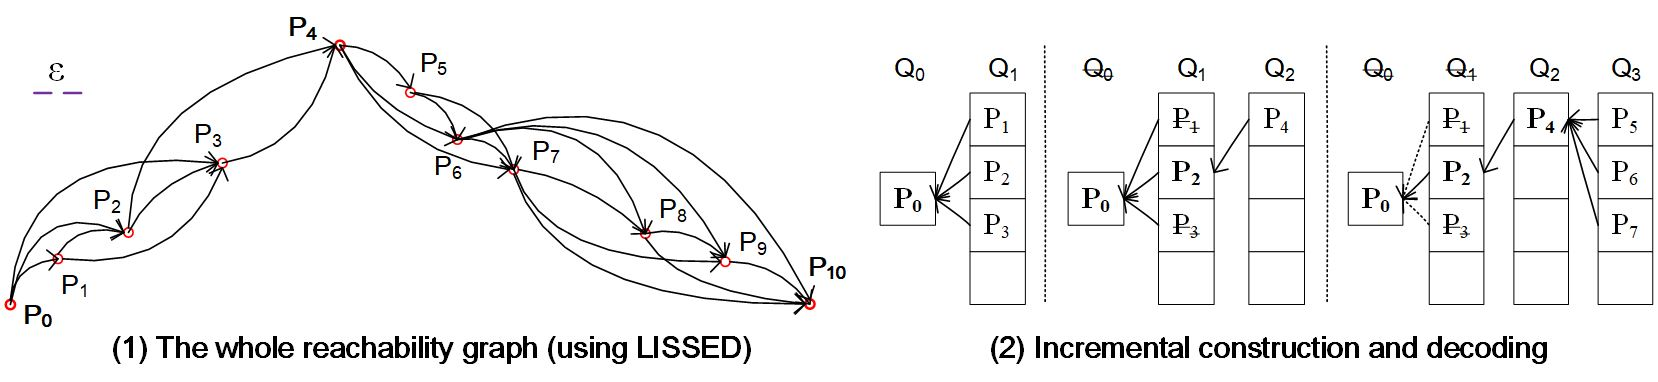
\includegraphics[scale=0.79]{Figures/Fig-DOTS.jpg}
	\vspace{-2ex}
	\caption{\small \textcolor{blue}{Example of algorithm \dagots~using \lissed with error bound of $\epsilon^2$, where (1) left is the supposed reachability graph of trajectory $\dddot{\mathcal{T}}[P_0, \ldots, P_{10}]$, and (2) right is the incremental construction of reachability graph and online decoding of the shortest path. Finally, the trajectory is compressed to four line segments.} }
	\vspace{-1ex}
	\label{fig:dots}
\end{figure*}



\begin{example}
	\label{exm-alg-dots}
	\textcolor{blue}{Figure~\ref{fig:dots} is an example of \dagots. The reachability graph is constructed layer by layer incrementally, and a part of the shortest path is determined before the whole graph is completely constructed. }
	%
	(a) \textcolor{blue}{Initially, $P_0$ is added to the first layer $Q_0$, and it is the only element in the layer.}
	%
	(b) \textcolor{blue}{Then, points $P_1$, $P_2$ and $P_3$ are in turn added to the second layer $Q_1$. Since $P_0$ does not have any new child point, \dagots~updates the status of $Q_1$ and outputs $P_2$ as it is the only \emph{alive} point in $Q_1$.}
	%
	(c) \textcolor{blue}{The process repeats. Point $P_4$ is added to layer $Q_2$, points $P_5$, $P_6$ and $P_7$ are added to layer $Q_3$, and so on.  }
	%
	(d) \textcolor{blue}{Finally, it outputs $4$ line segments $\vv{P_0P_2},\vv{P_2P_4},\vv{P_4P_7}$ and $\vv{P_7P_{10}}$.}
\end{example}

%%%%%%%%%%%%%%%%%%%%%%%%%%%%%%%%%%%%%%%%%%%%%%%%%%%%%%%%%%%%%%%%%%%%% END %%%%%%%%%%%%%%%%%%%%%%%%%%%%%%%%%%%%%%%%%%%%%%%%%%%%%%%%%%%%%%%%%%%%%%%%%%



\eat{%%%%%%%%%%%%%%%%%%%%%%%%%%%%%%%%%%%%%%%%%%%%%%%%%%%%%%%

\subsubsection{Sliding Window and Bottom-up}

The \swab algorithm~\cite{Keogh:online} is essentially the combination of the Sliding Window mechanism and the Bottom-up algorithm.
It keeps a window, $w[P_s, \ldots, P_{s+k-1}]$, of a fixed size of $k$.
The window size $k$ should be carefully chosen so that there are enough data points in the window to create about 5 or 6 line segments \cite{Keogh:online}.
Initially, $P_s=P_0$.
Next, the Bottom-Up algorithm, \eg \pavlidis algorithm, is applied to the points in the window, which merges the points into segments with the left-most segment being $\vv{P_sP_{s+i}}$, $i<k$.
Then $\vv{P_sP_{s+i}}$ is output, the window slides to right taking $P_{s+i+1}$ as the new start point of the window, and the Bottom-Up algorithm is applied again.
This process repeated until all points have been merged to segments.

The time complexity of \swab is a small constant factor worse than that of the standard Bottom-Up algorithm~\cite{Keogh:online}.
Also, it supports \sed. % as the standard Bottom-Up algorithm does.

\textcolor[rgb]{1.00,0.00,0.00}{Todo...dis-continuous line segments.}

} %%%%%%%%%%%%%%%%%%%%%%%%%%%%%%%%%%%%%% End of eat


\subsection{One-pass Algorithms}
%{One-pass algorithms that enforce the local checking policy}.
%The local checking policy \eat{, the key to achieve the \emph{one-pass} processing,} does not need a window to buffer the preview read points.
%Instead, it processes each point in a trajectory once and only once. % when compressing the trajectory.
%Obviously, the one-pass algorithms have a linear time complexity.

One-pass algorithms adopt local checking policies, and run in $O(n)$ time with an $O(1)$ space complexity. They are typically designed for specific distance metrics.

Reumann-Witkam (\rwa) \cite{Reumann:Strip} is a straightforward one-pass algorithm that builds a strip paralleling to the line connecting the first two points, then the points within this strip compose a section of the line.  \rwa is fast, but has a poor compression ratio.
Algorithm \operb~\cite{Lin:Operb} recently improves \rwa  by allowing dynamically adjustable strips, together with several detailed optimization techniques.
%
There is also algorithm \siped (\emph{sector intersection}) that converts \ped distance tolerances into angle tolerances to speed up the process, which is {\em completely overlooked} by existing trajectory compression studies,  but can be easily adopted for trajectory compression, as it is originally developed in fields of computational geometry and pattern recognition~\cite{Williams:Longest,Sklansky:Cone,Dunham:Cone, Zhao:Sleeve}.
\eat{
	Initially, Williams~\cite{Williams:Longest} and Sklansky and Gonzalez \cite{Sklansky:Cone} proposed linear time algorithms based on the idea of ``cone intersection" in a plane, then Dunham \cite{Dunham:Cone} extended these algorithms, and the Sleeve algorithm \cite{Zhao:Sleeve} in the cartographic discipline essentially applied the same idea as \siped but alternatively called it ``sector intersection".
}%
These algorithms are dedicatedly designed  for \ped. {\em Algorithms \operb and \siped have good compression ratios, and, hence, we choose them as the representatives of  one-pass algorithms using \ped}.


Algorithm Linear Dead Reckoning (\ldr) for position tracking \cite{Trajcevski:DDR} follows the similar routine as \rwa except that it uses \sed and assumes a velocity ${\vv{v}}$ for each section. \textcolor{blue}{\cite{Trajcevski:DDR} proves that if \ldr uses $\epsilon/2$ as the threshold in position tracking, then its output trajectory has a max error not greater than $\epsilon$ to the original trajectory. Thus, it can be treated as a trajectory simplification algorithm as well.}
It has poor compression ratios because both the value and the direction of velocity ${\vv{v}}$ are pre-defined and fixed between two updates, \myblue{and it indeed uses a half $\epsilon$}.
Recently algorithm \cised~\cite{Lin:Cised} extends the \textit{sector intersection} method \siped from a 2D space to a spatio-temporal 3D space.
These one-pass algorithms are dedicatedly designed for \sed. {\em As algorithm \cised has a compression ratio close to algorithm \dpa using \sed, we choose it as the representative of one-pass algorithms using \sed}.


{Direction range intersection} approaches are similar to  \emph{sector intersection} methods except that they are designed for \dad, and {\em we choose \intersec \cite{Long:Direction} and \interval \cite{Ke:Interval} as the representatives of one-pass algorithms using \dad}.

\textcolor{blue}{Algorithms \siped, \ldr, \operb, \cised and \intersec share a common idea, \ie using a half-$\epsilon$ to implement the strong simplification to ensure that the max error does not exceed $\epsilon$. In the sequel, we shall discuss that the half-$\epsilon$ of \siped and \cised can be extended to the full-$\epsilon$ with some small modifications, along the similar way that \interval extends \intersec. }

\eat{%%%%%%%%%%%%%%%%%%%%%%%%%%%%%%%%%%%%%%%%%%%%%%%%%%%%%%%
	
	The $n^{th}$ point routine and the routine of random-selection of points \cite{Shi:Survey} are two naive one-pass algorithms.
	In these routines, for every fixed number of consecutive points along the line, the $n^{th}$ point and one random point among them are retained, respectively.
	They run fast, however, they are not error bounded.
	
	\subsubsection{Reumann-Witkam and LDR}
	
	\begin{figure*}[tb!]
		\centering
		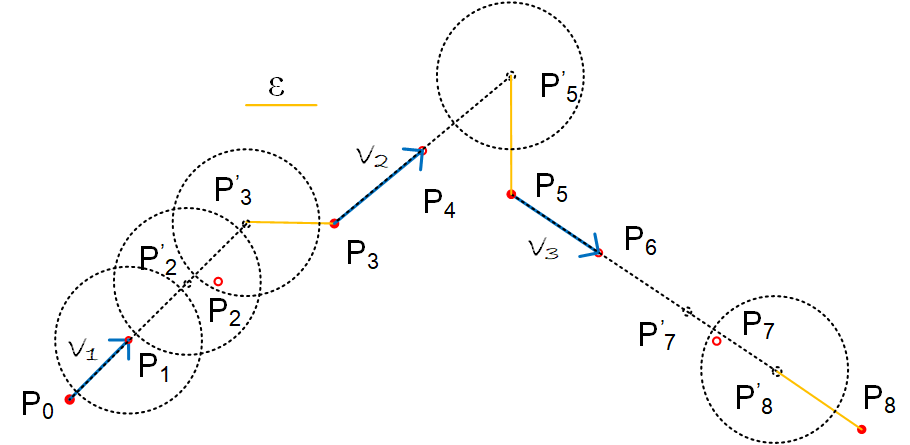
\includegraphics[scale=0.66]{Figures/Fig-LDR.jpg}
		\vspace{-1ex}
		\caption{\small The trajectory $\dddot{\mathcal{T}}[P_0, \ldots, P_{10}]$ is compressed by the Reumann-Witkam and Linear Dead Reckoning algorithms to four and eight line segments, respectively.}
		\vspace{-2ex}
		\label{fig:ldr}
	\end{figure*}
	
	In Reumann-Witkam\cite{Reumann:Strip}, the input data is divided into sections by strips.
	Initially, the first strip, with the width of $2*\epsilon$, takes the line $\vv{P_0P_1}$ connecting the first two points, $P_0$ and $P_1$ as its middle line.
	Then the strip is expending over the line into the direction of its initial tangent, covering the succeed points, $P_2, \ldots, P_{j}$, until the strip hits the line $\vv{P_jP_{j+1}}$ (meaning that the next point $P_{j+1}$, $j>1$, is out side of the strip).
	The points, $[P_0, \ldots, P_{j}]$, within this strip compose a section. The first and last points of the section, \ie $P_0,P_{j}$, are output, and those points between them are removed.
	The last point $P_{j}$ is the initial point of the next strip.
	The whole process is repeated until the strip contains the end point $P_n$ of the input data.
	The Reumann-Witkam is a one-pass algorithm.
	
	{The Linear Dead Reckoning (LDR)\cite{Lange:Tracking} for position tracking follows the similar routine as the Reumann-Witkam algorithm except that it assumes a velocity ${\vv{v}}$ for each section and uses \sed instead of \ped in distance checking.
		Moreover, the authors of \cite{Trajcevski:DDR} proved that LDR is also suitable for online spatio-temporal compression as long as the tolerance threshold of the algorithm is set to $\epsilon/2$.}
	
	\begin{example}
		\label{exm-alg-strip}
		In Figure~\ref{fig:ldr}, the trajectory $\dddot{\mathcal{T}}[P_0, \ldots, P_{10}]$ is compressed
		%
		(1) by the Reumann-Witkam to four line segments $\vv{P_0P_2}$, $\vv{P_2P_4}$, $\vv{P_4P_7}$ and $\vv{P_7P_{10}}$. First, a strip with width $2\epsilon$ is built parallel to the line $\vv{P_0P_1}$, then the strip is extended over the line and includes point $P_2$. Because $P_3$ is outside of the strip, $P_2$ becomes the end point of the first section and the start point of the second section.
		%
		(2) by the Linear Dead Reckoning algorithm to eight line segments $\vv{P_0P_1}$, $\vv{P_1P_2}$, $\vv{P_2P_3}$, $\vv{P_3P_4}$, $\vv{P_4P_5}$, $\vv{P_5P_7}$, $\vv{P_7P_8}$ and $\vv{P_8P_{10}}$. First, an initial velocity ${\vv{v}_0}$ is set to $|P_0P_1|/(t_1-t_0)$. Then the synchronized point $P'_2$ of $P_2$ is estimated based on the velocity ${\vv{v}_0}$ and time of $P_2$, \ie ${v}_0 * (t_2-t_0)$. Because the \sed from $P_2$ to the line $\vv{P_0P'_2}$ , \ie $|P_2P'_2|$, is great than $\epsilon/2$, the algorithm outputs $\vv{P_0P_1}$ and starts the next section.
	\end{example}
	
}%%%%%%%%%%%%%%%%%%%%%%%%%%%%%%%%%%%%%%%%%%%%%%%%%%%%%%%End of Eat


\subsubsection{{Algorithm \operb Using \ped} \cite{Lin:Operb}}
It designs a local distance checking method to dynamically adjust the direction of line segments to achieve an effective one-pass process. \textcolor{blue}{It has strong and weak versions, called \operb and \operb-A, respectively. \operb-A shares the same routine as \operb except that it applies a lazy output policy and allows data interpolations.}

Consider an error bound $\epsilon$ and a sub-trajectory $\dddot{\mathcal{T}_s}[P_s,$ $\ldots, P_{s+k}]$.
\operb dynamically maintains a directed line segment $\mathcal{L}_i$ ($i\in[1,k]$), whose start point is fixed with $P_s$ and its end point is identified (may not in $\{P_s, \ldots, P_{s+i}\}$) to {\em fit} all the previously processed points $\{P_s, \ldots, P_{s+i}\}$.
The directed line segment $\mathcal{L}_i$ is built by a function named \emph{fitting function $\mathbb{F}$}, such that when a new point $P_{s+i+1}$ is considered, only its distance to the directed line segment $\mathcal{L}_i$ is checked, instead of checking the distances of all or a subset of data points of $\{P_{s}, \ldots, P_{s+i}\}$ to $\mathcal{R}_{i+1}$ = $\vv{P_sP_{s+i+1}}$ as the global distance checking does.
During processing, if the distance of point $P_{s+i}$ to the directed line segment $\mathcal{L}_{i-1}$ is larger than the threshold, then a directed line segment, start from $P_s$, is generated and output;
otherwise, the directed line segment $\mathcal{L}_i$ is updated by the fitting function $\mathbb{F}$, as follows.

\begin{small}
	\vspace{-1ex}
	\begin{equation*}
	\label{equ-function}
	\left\{
	\hspace{1ex}\begin{aligned}
	&\left[
	\begin{aligned}
	% & |\mathcal{L}_{i}| = |\mathcal{R}_{i-1}|    \\
	% & \mathcal{L}_{i}.\theta = \mathcal{R}_{i-1}.\theta\\
	& \mathcal{L}_{i} = \mathcal{L}_{i-1}\\
	\end{aligned}
	\right]\hspace{12.5ex}~when~(|\mathcal{R}_{i}| - |\mathcal{L}_{i-1}|) \le \frac{\epsilon}{4}   \\
	&\hspace{-1.5ex}\left[
	\begin{aligned}
	& |\mathcal{L}_{i}|  = j*{\epsilon}/{2} \\
	& \mathcal{L}_{i}.\theta = \mathcal{R}_{i}.\theta    \\
	\end{aligned}
	\right]\hspace{8.5ex}~when~|\mathcal{R}_{i}| >  \frac{\epsilon}{4}~\And~|\mathcal{L}_{i-1}|=0    \\
	&\hspace{-1.5ex}\left[
	\begin{aligned}
	& |\mathcal{L}_{i}|  = j*{\epsilon}/{2}\\
	& \mathcal{L}_{i}.\theta = \mathcal{L}_{i-1}.\theta + f(\mathcal{R}_i,\mathcal{L}_{i-1})*\arcsin(\frac{ped(P_{s+i}, \mathcal{L}_{i-1})}{j*\epsilon/2})/j \\	
	% & \theta^- = \mathcal{L}_{i-1}.\theta - \arcsin(\frac{d(P_i, \mathcal{L}_{i-1})}{j*\epsilon/2})/j \\	
	% & \mathcal{L}_{i}.\theta = \arg_{\mathcal{L}_{i}.\theta}\min({d(P_{i+1}, \mathcal{L}_{i}}), \mathcal{L}_{i}.\theta \in\{\theta^+,\theta^-\})\\	
	\end{aligned}
	\right]\hspace{0ex}else\\
	\end{aligned}
	\right.
	\end{equation*}
	\vspace{0ex}
\end{small}


\ni where (a) $1 \le i \le k+1$; (b) $\mathcal{R}_{i-1}$ = $\vv{P_sP_{s+i-1}}$, is the directed line segment whose end point $P_{s+i-1}$ is in $\dddot{\mathcal{T}_s}[P_s, \ldots, P_{s+k}]$; (c) $\mathcal{L}_{i}$ is the directed line segment built by fitting function $\mathbb{F}$ to fit sub-trajectory $\dddot{\mathcal{T}_s}[P_s, \ldots, P_{s+i}]$ and $\mathcal{L}_{0}$ = $\mathcal{R}_{0}$; (d) $j = \lceil(|\mathcal{R}_{i}|*2/\epsilon - 0.5)\rceil$; (e) $f()$ is a sign function such that $ f(\mathcal{R}_i,\mathcal{L}_{i-1})$ = $1$ if the included angle $\angle(\mathcal{R}_{i-1}, \mathcal{R}_{i})$ = $(\mathcal{R}_i.\theta - \mathcal{L}_{i-1}.\theta)$ falls in the range of $(-2\pi, -\frac{3\pi}{2}]$, $[-\pi, -\frac{\pi}{2}]$, $[0, \frac{\pi}{2}]$ and $[\pi, \frac{3\pi}{2})$, and $f(\mathcal{R}_i,\mathcal{L}_{i-1})$ = $-1$, otherwise; (f) $\epsilon/2$ is a step length to control the increment of $|\mathcal{L}|$.
%
Optimizations are developed to achieve better compression ratios.


\begin{example}
	\label{exm-alg-operb}
	Figure~\ref{fig:operb} is a running example of the \operb algorithm compressing the same trajectory $\dddot{\mathcal{T}}[P_0, \ldots, P_{10}]$.
	(1) It takes $P_0$ as the start point, reads $P_1$ and sets $\mathcal{L}_1$ = $\vv{P_0P_1}$.
	(2) It reads $P_2$. The distance from $P_2$ to $\mathcal{L}_1$ is less than the threshold, thus, it updates $\mathcal{L}_1$  to $\mathcal{L}_2$ by the fitting function $\mathbb{F}$.
	(3) It reads $P_3$ and $P_4$, and updates $\mathcal{L}_2$ to $\mathcal{L}_3$ and $\mathcal{L}_3$ to $\mathcal{L}_4$, respectively.
	(4) It reads $P_5$. The distance from $P_5$ to $\mathcal{L}_4$ is larger than the threshold, thus, it outputs $\vv{P_0P_4}$ and starts the next section taking $P_4$ as the new start point.
	(5) The process continues until all points have been processed. At last, the algorithm outputs two continuous line segments $\vv{P_0P_4}$ and $\vv{P_4P_{10}}$.
\end{example}


\begin{figure}[tb!]
	\centering
	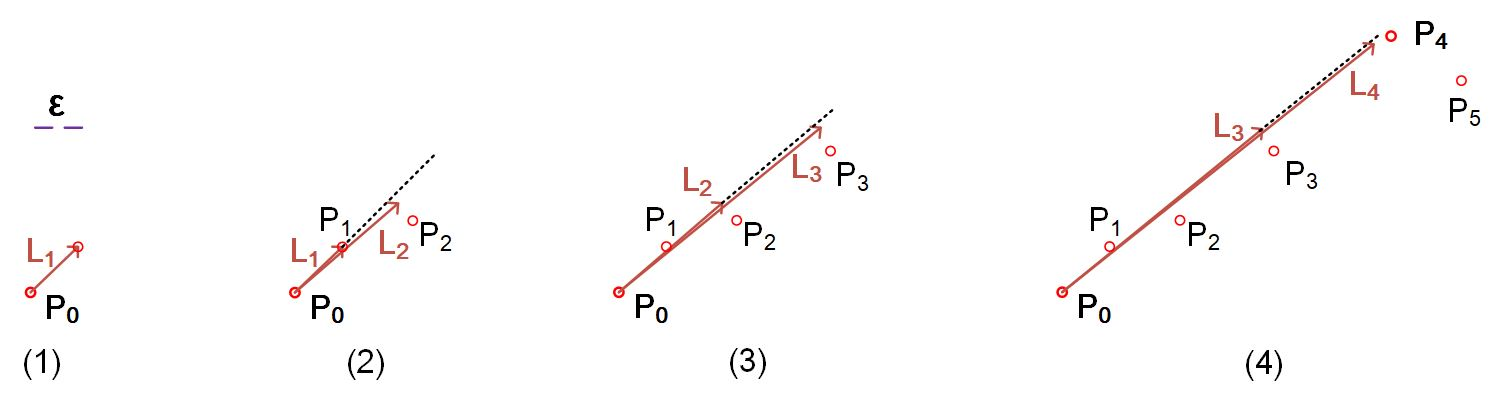
\includegraphics[scale=0.66]{Figures/Fig-OPER.jpg}
	\vspace{-1ex}
	\caption{\small The trajectory $\dddot{\mathcal{T}}[P_0, \ldots, P_{10}]$ is compressed by the \operb algorithm using \ped to two line segments.}
	\vspace{-1ex}
	\label{fig:operb}
\end{figure}


\subsubsection{Algorithm \siped Using \ped \cite{Williams:Longest, Sklansky:Cone, Dunham:Cone, Zhao:Sleeve}}
It develops a concept of ``Sector'' \cite{Williams:Longest, Sklansky:Cone, Dunham:Cone, Zhao:Sleeve}, which converts the distance tolerance into the angle change tolerance for checking  points.

Given a sequence of points $[P_{s}, P_{s+1}, \ldots, P_{s+k}]$ and an error bound $\epsilon$,
for the start data point $P_s$, any point $P_{s+i}$ and $|\vv{P_sP_{s+i}}|>\epsilon$ ($i\in[1, k]$), there are two directed lines $\vv{P_sP^u_{s+i}}$ and $\vv{P_sP^l_{s+i}}$ such that $ped(P_{s+i}, \vv{P_sP^u_{s+i}})$ $=$ $ped(P_{s+i}, \vv{P_sP^l_{s+i}}) = \epsilon$ and either ($\vv{P_sP^l_{s+i}}.\theta < \vv{P_sP^u_{s+i}}.\theta ~and~\vv{P_sP^u_{s+i}}.\theta - \vv{P_sP^l_{s+i}}.\theta <\pi$) or ($\vv{P_sP^l_{s+i}}.\theta > \vv{P_sP^u_{s+i}}.\theta ~and~ \vv{P_sP^u_{s+i}}.\theta - \vv{P_sP^l_{s+i}}.\theta < -\pi)$. Indeed, they form a \emph{sector} \sector{(P_s, P_{s+i}, \epsilon)} that takes $P_s$ as the center point and $\vv{P_sP^u_{s+i}}$ and $\vv{P_sP^l_{s+i}}$ as the borderlines.
%
There exists a data point $Q$ such that for any data point $P_{s+i}$ ($i \in [1, ... k]$), its perpendicular Euclidean distance to
directed line $\overline{P_sQ}$ is not greater than the error bound $\epsilon$ if and only if the $k$ sectors \sector{(P_s, P_{s+i}, \epsilon)} ($i\in[1,k]$) share common data points other than $P_s$, \ie $\bigsqcap_{i=1}^{k}$\sector{(P_s, P_{s+i}, \epsilon)} $\ne \{P_s\}$ \cite{Williams:Longest, Sklansky:Cone,Zhao:Sleeve}.
%
Here, point $Q$ may not belong to $\{P_{s}, P_{s+1},$ $\ldots, P_{s+k}\}$.
However, if $Q$ must be a point selected from the original points, in other words, point $P_{s+i}$ ($1\le i\le k$) is chosen as $Q$, then
for any point $P_{s+j}$ ($j \in [1, ... i]$), its \ped to
line segment $\overline{P_sP_{s+i}}$ is not greater than the error bound $\epsilon$ if $\bigsqcap_{j=1}^{i}$\sector{(P_s, P_{s+j}, \epsilon/2)} $\ne \{P_s\}$, as pointed out in \cite{Zhao:Sleeve}.
That is, {\em these sector intersection based algorithms can be easily adopted for trajectory compression}.
In practice, it is a good choice to set the point $Q$ as the point among all points in $[P_{s}, P_{s+1}, \ldots, P_{s+k}]$ that has the longest distance to $P_s$.


The original \siped uses a half sector, $\frac{\epsilon}{2}$-\sector, which may limit its compression performance. However, it can further be extended to a full ${\epsilon}$-\sector ~ by adding a constraint. That is, for any point $P_{s+j}$ ($j \in [1, ... i]$), its \ped to
line segment $\overline{P_sP_{s+i}}$ is not greater than the error bound $\epsilon$ if $ P_{s+i} \ne {P_s}$ and $P_{s+i}\in \bigsqcap_{j=1}^{i-1}$\sector{(P_s, P_{s+j}, \epsilon)}, \ie $P_{s+i}$ lives in the common intersection of the preview full \emph{sectors}.



\begin{example}
	\label{exm-alg-sleeve}
	Figure~\ref{fig:sleeve} is a running example of algorithm \siped($\frac{\epsilon}{2}$) taking as input the same trajectory $\dddot{\mathcal{T}}[P_0, \ldots, P_{10}]$. At the beginning, $P_0$ is the first start point, and points $P_1$, $P_2$, $P_3$, etc., each has a narrow \emph{sector}.
	For example, the narrow \emph{sector} $\mathcal{S}$($P_0$, $P_{3}$, $\epsilon/2$) takes $P_0$ as the center point and $\vv{P_0P^u_{3}}$ and $\vv{P_0P^l_{3}}$ as the borderlines.
	Because $\bigsqcap_{i=1}^{4}\mathcal{S}(P_0, P_{0+i}, \epsilon/2) \ne \{P_0\}$ and $\bigsqcap_{i=1}^{5}\mathcal{S}(P_0, P_{0+i}, \epsilon/2) = \{P_0\}$, $\vv{P_0P_4}$ is output and $P_4$ becomes the start point of the next section.
	At last, the algorithm outputs two continuous line segments $\vv{P_0P_4}$ and $\vv{P_4P_{10}}$.
\end{example}

\begin{figure}[tb!]
	\centering
	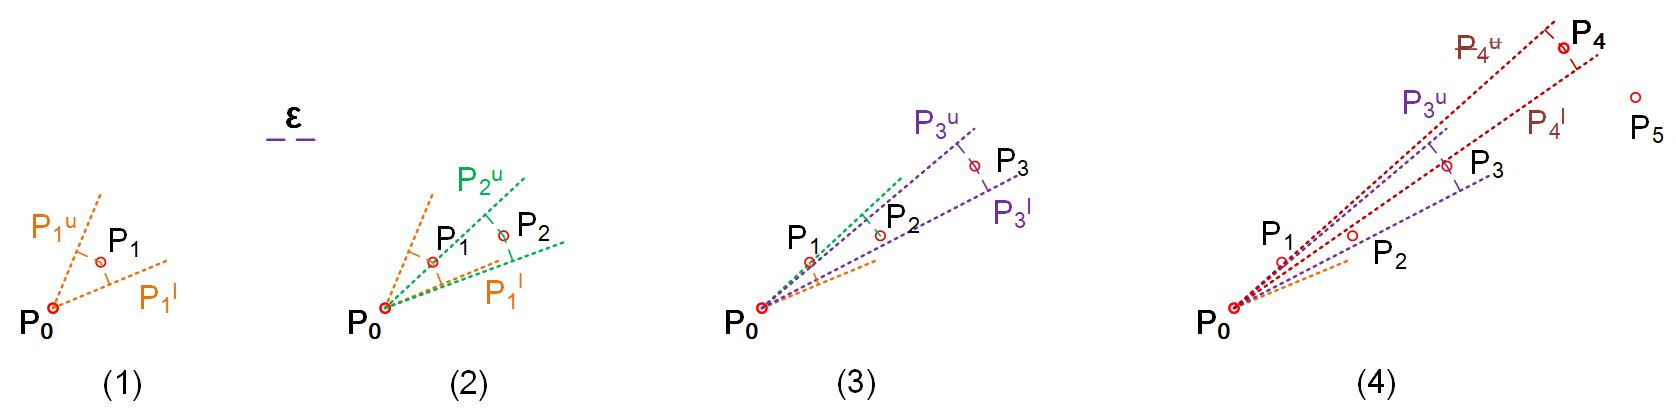
\includegraphics[scale=0.66]{Figures/Fig-sleeve.jpg}
	\vspace{-2ex}
	\caption{\small The trajectory $\dddot{\mathcal{T}}$ is compressed by the sector intersection algorithm using \ped to two line segments.}
	\vspace{-1ex}
	\label{fig:sleeve}
\end{figure}




\subsubsection{Algorithm \cised Using \sed \cite{Lin:Cised}}
It develops an idea of \textit{spatio-temporal cone} that extends the \textit{sector intersection} method \cite{Williams:Longest, Sklansky:Cone, Dunham:Cone, Zhao:Sleeve} from an \textcolor{blue}{\em x-y} 2D space to an \textcolor{blue}{\em x-y-t} spatio-temporal 3D space.
\textcolor{blue}{Note that for computer graphics and cartography, there is another 3D space, \ie \emph{x-y-z} 3D space, where {\em z} is the height. There are studies \cite{Barequet:3D, Eu:Ln3D} for solving the \emph{min-\#} and \emph{min-$\epsilon$} problems in the \emph{x-y-z} 3D space, \eg \cite{Barequet:3D} extends the \textit{sector intersection} method to the \textit{off-line ball-inclusion testing} in the \emph{x-y-z} 3D space, so as to develop efficient near quadratic time algorithms.} %

Given a sub-trajectory $[P_s,...,P_{s+k}]$ and an error bound $\epsilon$, any point $P'_{s+i}$ ($0< i \le k$) on the plane $P.t-P_{s+i}.t = 0$ is a synchronized data point of $P_{s+i}$. For all $P'_{s+i}$ in the plane satisfying $|P_{s+i}P'_{s+i}| \le \epsilon$, they form a \textit{synchronous circle $\mathcal{O}(P_{s+i}, \epsilon)$} of $P_{s+i}$ with $P_{s+i}$ as its center and $\epsilon$ as its radius.
%
A spatio-temporal cone (or simply \textit{cone}) of a data point $P_{s+i}$ ($1\le i\le k$) in $\dddot{\mathcal{T}}_s$ \wrt a point $P_s$ and an error bound $\epsilon$, denoted as \cone{(P_s, \mathcal{O}(P_{s+i}, \epsilon))}, or \cone{_{s+i}} in short, is an oblique circular cone such that point $P_s$ is its apex and the synchronous circle $\mathcal{O}(P_{s+i}, \epsilon)$ is its base.
%
Then, there exists a point $Q$ such that $Q.t = P_{s+k}.t$ and $sed(P_{s+i}, \vv{P_sQ})\le \epsilon$ for each $i \in [1,k]$ if and only if $\bigsqcap_{i=1}^{k}$\cone{(P_s, \mathcal{O}(P_{s+i}, \epsilon))} $\ne \{P_s\}$.
%
Like \textit{sector intersection} methods, point $Q$ may also not belong to $\{P_{s}, P_{s+1},$ $\ldots, P_{s+k}\}$.
\textcolor{blue}{If point $Q$ is not necessarily in  $\{P_{s}, P_{s+1},$ $\ldots, P_{s+k}\}$, then this algorithm is a weak simplification, named \cised-W that uses a full-$\epsilon$ cone.}
If point $Q$ must be $P_{s+i}$ ($1\le i\le k$), then for any point $P_{s+j}$ ($j \in [1, ... i]$), its \sed to line segment $\overline{P_sP_{s+i}}$ is not greater than the error bound $\epsilon$ if
$\bigsqcap_{j=1}^{i}$\cone{(P_s, P_{s+j}, \epsilon/2)} $\ne \{P_s\}$ as pointed out in \cite{Lin:Cised}.
\textcolor{blue}{This algorithm, named \cised($\frac{\epsilon}{2}$) that uses a half-$\epsilon$ cone, belongs to strong simplification.}
\textcolor{blue}{Moreover, \cised($\frac{\epsilon}{2}$) can also be extended to \cised(${\epsilon}$), another strong version that uses a full-${\epsilon}$ cone,} by adding a constraint that $P_{s+i}$ lives in the common intersection of the preview full \emph{cones}.

In addition, because these spatio-temporal cones have the same apex $P_s$, the checking of their intersection can be computed by a much simpler way, \ie the checking of the intersection of cone projection circles on a plane, and a circle is further approximated with its $m$-edge inscribed regular polygon, whose intersection can be computed more efficiently. %



\eat{
	\begin{figure}[tb!]
		\centering
		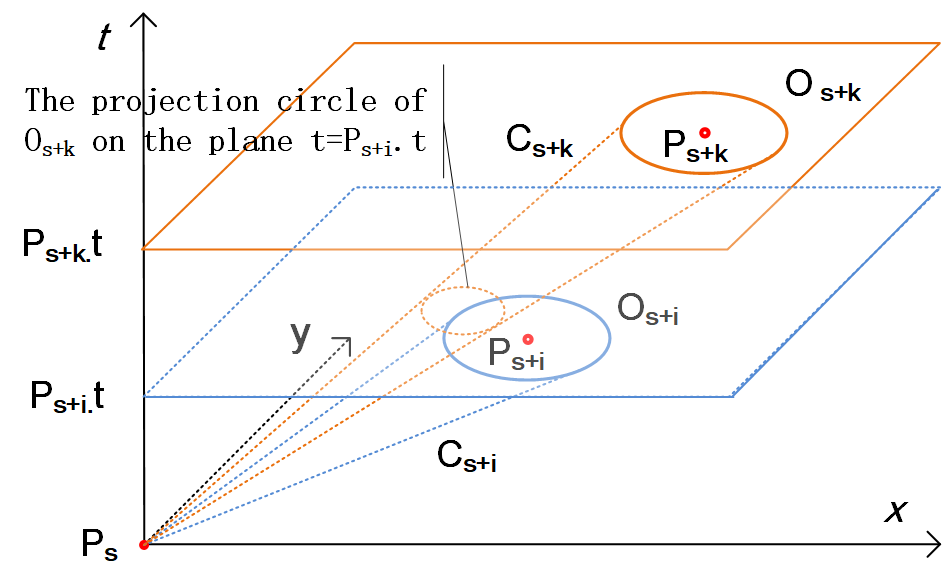
\includegraphics[scale=0.66]{Figures/Fig-CIS.jpg}
		\vspace{-3ex}
		\caption{\small Examples of spatio-temporal cones.} % in a 3D Cartesian coordinate system
		\vspace{-2ex}
		\label{fig:cis}
	\end{figure}
}


%%%%%%%%%%%%%%% example of Algorithm CISED
\begin{figure}[tb!]
	\centering
	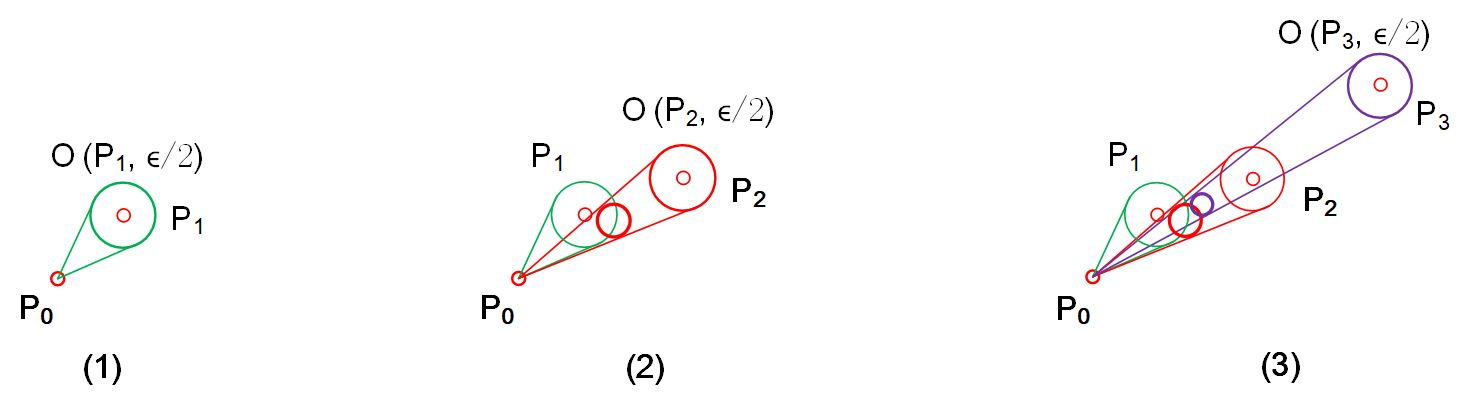
\includegraphics[scale=0.66]{Figures/Fig-Conest.jpg}
	\vspace{-1ex}
	\caption{\small A running example of the \cised algorithm. The points and the oblique circular cones are projected on an x-y space. }%The trajectory $\dddot{\mathcal{T}}[P_0, \ldots, P_{10}]$ is compressed into four line segments.
	\vspace{-2ex}
	\label{fig:exm-conest}
\end{figure}
%%%%%%%%%%%%%%%%

\begin{example}
	\label{exm-alg-conest}
	Figure~\ref{fig:exm-conest} shows a running example of algorithm \cised($\frac{\epsilon}{2}$) for compressing the trajectory \trajec{T} in Figure~\ref{fig:dp}.
	For convenience, we project the points and the oblique circular cones on an x-y space.
	%	
	(1) After initialization, the \cised algorithm reads point $P_1$ and builds a narrow \emph{oblique circular cone}~\cone{(P_0, \mathcal{O}(P_{1}, \epsilon/2))}, taking $P_0$ as its apex and \circle{(P_1, \epsilon/2)} as its base (green dash). The \emph{circular cone} is projected on the plane $P.t-P_1.t=0$, and the inscribe regular polygon $\mathcal{R}_1$ of the projection circle is returned. As $\mathcal{R}^*$ is empty, $\mathcal{R}^*$ is set to $\mathcal{R}_1$.
	%	
	(2) The algorithm reads $P_2$ and builds \cone{(P_0, \mathcal{O}(P_{2}, \epsilon/2))} (red dash). The \emph{circular cone} is also projected on the plane $P.t-P_1.t=0$ and the inscribe regular polygon $\mathcal{R}_2$ of the projection circle is returned. As $\mathcal{R}^*=\mathcal{R}_1$ is not empty, $\mathcal{R}^*$ is set to the intersection of $\mathcal{R}_2$ and $\mathcal{R}^*$, which is $\mathcal{R}_1 \bigsqcap \mathcal{R}_2 \ne \emptyset$.
	%	
	(3) For point $P_3$, the algorithm runs the same routine as $P_2$ until the intersection of $\mathcal{R}_3$ and $\mathcal{R}^*$ is $\emptyset$. Thus, a line segment $\vv{P_0P_2}$ is generated, and the process of a new line segment is started, taking $P_2$ as the new start point and $P.t-P_3.t=0$ as the new projection plane.
	%	
	(4) At last, the algorithm outputs four continuous line segments, \ie $\{\vv{P_0P_2}$, $\vv{P_2P_4}$, $\vv{P_4P_{7}}$, $\vv{P_7P_{10}}\}$. %\eop
\end{example} 	


\begin{figure}[tb!]
	\centering
	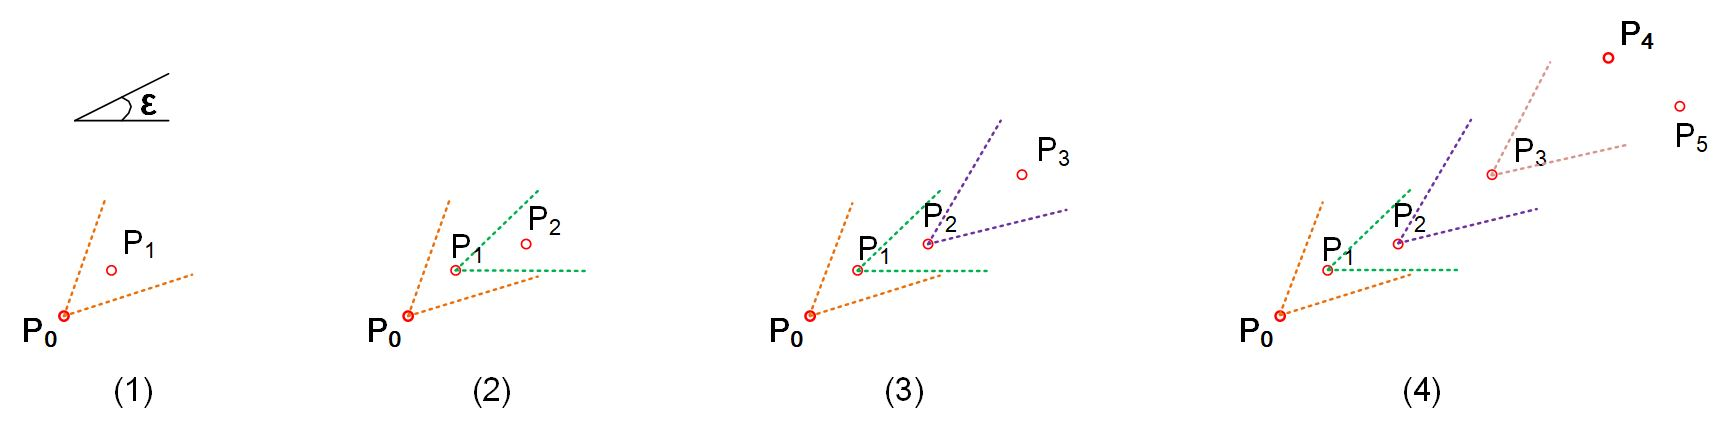
\includegraphics[scale=0.66]{Figures/Fig-interval.jpg}
	\vspace{-1ex}
	\caption{\small The trajectory $\dddot{\mathcal{T}}$ is compressed by the interval algorithm using \dad to two line segments.}
	\vspace{-1ex}
	\label{fig:interval}
\end{figure}




\subsubsection{Algorithms \intersec \cite{Long:Direction} and \interval \cite{Ke:Interval} Using \dad}
It designs a \emph{direction range} for each line segment connecting two neighboring points, then checks the common intersection of those \emph{direction ranges} as a way similar to the \emph{sector intersection} approach \cite{Williams:Longest, Sklansky:Cone, Dunham:Cone, Zhao:Sleeve}.

Given a direction line segment $\mathcal{L}$ and an angle $\epsilon$, the \emph{direction range} denoted by $range(\mathcal{L}.\theta, \epsilon)$ is $[\mathcal{L}.\theta-\epsilon, \mathcal{L}.\theta+\epsilon]$, which denotes the varying range of a directed line segment originated from the origin when it is rotated anti-clockwise from $\theta_1$ to $\theta_2$  \cite{Long:Direction}.
%
The {common intersection} of \emph{direction ranges} of directed line segments $\{\vv{P_sP_{s+1}}, \vv{P_{s+1}P_{s+2}}, ..., \vv{P_{s+k-1}P_{s+k}}\}$ \wrt $\epsilon$ is $\bigsqcap_{i=1}^{k}Range(\vv{P_{s+i-1} P_{s+i}}.\theta, \epsilon)$.
%denoted by $ComSub(\{\vv{P_sP_{s+1}}, \vv{P_{s+1}P_{s+2}}, ..., \vv{P_{s+k-1}P_{s+k}}\}, \epsilon)$,

Algorithm \intersec\cite{Long:Direction} uses a half range, and shows that if the {common intersection} $\bigsqcap_{i=1}^{k}range(\vv{P_{s+i-1} P_{s+i}}.\theta, \epsilon/2)$ is not empty, then the angle between $\vv{P_{s+i-1}P_{s+i}}$ and $\vv{P_sP_{s+k}}$ for all $i\in [1, k]$ is not larger than $\epsilon$.
%
Recently, algorithm \interval \cite{Ke:Interval} extends \intersec from half to full ranges, by showing that if the {common intersection} $\bigsqcap_{i=1}^{k}range(\vv{P_{s+i-1} P_{s+i}}.\theta, \epsilon)$ is not empty and $\vv{P_sP_{s+k}}.\theta$ falls in the {common intersection}, then the angle between $\vv{P_{s+i-1}P_{s+i}}$ and $\vv{P_sP_{s+k}}$ for all $i\in [1, k]$ is not larger than $\epsilon$.


\begin{example}
	\label{exm-alg-interval}
	Figure~\ref{fig:interval} is a running example of the \emph{interval} method taking as input the same trajectory $\dddot{\mathcal{T}}[P_0, \ldots, P_{10}]$. At the beginning, $P_0$ is the first start point, and points $P_1$, $P_2$, $P_3$, etc., each has a \emph{direction range} $Range(\vv{P_0P_1}, \epsilon)$, $Range(\vv{P_1P_2}, \epsilon)$, $Range(\vv{P_2P_3}, \epsilon)$, etc., respectively.
	%
	Because $\bigsqcap_{i=1}^{4}Range(\vv{P_{0+i-1}P_{0+i}}, \epsilon) \ne \phi$ and $\vv{P_0P_{4}}.\theta$ falls in the \emph{common sub-interval}, and $\bigsqcap_{i=1}^{5}Range(\vv{P_{0+i-1}P_{0+i}}, \epsilon) = \phi$, $\vv{P_0P_4}$ is output and $P_4$ becomes the start point of the next section.
	At last, the algorithm outputs two continuous line segments $\vv{P_0P_4}$ and $\vv{P_4P_{10}}$.
\end{example}













{\section{Trajectory Aging}}
\label{sec-aging}

Suppose that we have compressed a trajectory $\dddot{\mathcal{T}_0}$ to $\overline{\mathcal{T}}_1$ using any \lsa algorithm $\mathcal{A}$ with an error bound $\epsilon_1$. As time evolves, we may need to further compress $\overline{\mathcal{T}}_1$ to an even coarser trajectory $\overline{\mathcal{T}}_2$.
What are the relationships among $\overline{\mathcal{T}}_2$, $\overline{\mathcal{T}}_1$ and $\dddot{\mathcal{T}_0}$? And what is the right way to get the coarser trajectory $\overline{\mathcal{T}}_2$?
{What line simplification algorithms should we use in the first and second rounds of simplifications? If the first round of simplification uses algorithm $\mathcal{A}_1$, can we use algorithm $\mathcal{A}_2$ in the second round? How to set the parameter of error bounds in these simplifications? And after multiple rounds of simplifications, does the coarse trajectory still have bounded errors \wrt the original trajectory?}
%
This section is to answer these questions from the views of friendliness \cite{Cao:Spatio} (Section \ref{sec-aging-friend}) and errors (Section \ref{sec-aging-safe}).
Note that (1) if we get $\overline{\mathcal{T}}_1$ and $\overline{\mathcal{T}}_2$ by optimal algorithms \wrt error bounds $\epsilon_1$ and $\epsilon_2$, respectively, then $\overline{\mathcal{T}}_2$ may not be the optimal one of $\dddot{\mathcal{T}_0}$ \wrt any error bound \cite{Cao:Spatio}, {and (2) as \lissed is a special case of \sed, we refer to the \sed errors rather than the \lissed errors when we talk about aging friendliness and errors of algorithms using \lissed (recall that \emph{if the \lissed error bound of such an algorithm  is set to $\epsilon^2$, then its maximal \sed error is not greater than $\epsilon$})}. The major results are summarized in \mytable{tab:summary-data-aging}.
%Hence, we focus on sub-optimal error bounded trajectory simplification algorithms only.


\subsection{Friendliness of Data Aging}
\label{sec-aging-friend}
We first discuss the relationship between $\overline{\mathcal{T}}_1$ and $\overline{\mathcal{T}}_2$ from the view of friendliness, which was defined in \cite{Cao:Spatio}, but was seldom discussed later.
	
\stitle{Aging friendly \cite{Cao:Spatio}}. {An \lsa algorithm $\mathcal{A}$ is aging friendly with respect to a distance metric $\mathcal{M}$ if for every $\epsilon_1$ and every $\epsilon_2$ such that $\epsilon_1 < \epsilon_2$, and for every trajectory $\dddot{\mathcal{T}}$, $\mathcal{A}(\dddot{\mathcal{T}}, \epsilon_2, \mathcal{M})= \mathcal{A}(\mathcal{A}(\dddot{\mathcal{T}}, \epsilon_1, \mathcal{M}), \epsilon_2, \mathcal{M})$.}

Cao et al. proved in \cite{Cao:Spatio} that ``an optimal line simplification algorithm is not aging-friendly \wrt~the \ped and \sed'', and ``the top-down algorithm \dpa is aging friendly \wrt~\ped and \sed'' on the premise that the second run of \dpa takes as input the whole simplified trajectory produced by the first run.
However, algorithms other than the optimal algorithms and the top-down algorithm \dpa with distance metrics other than \ped and \sed are not discussed in \cite{Cao:Spatio}, thus, their effectiveness in data aging remains an open problem.
In the rest, we  present a full picture of this problem, starting from the optimal algorithms coupling with \dad.

\begin{table}
	\renewcommand{\arraystretch}{1.20}
	\vspace{-1ex}
	\caption{\small Aging friendliness and error bounds of line simplification algorithms for data aging}
	\label{tab:summary-data-aging}
	\centering
	\scriptsize
	\begin{tabular}{|c|c|c|c|c|}
		\hline
		{\bf{Algorithms}} &\bf{Distance Metrics} & \bf{Aging Friendliness} &  {\bf{Error Bounds}}  \\		
		\hline

		{\multirow{2}*{{\opt} algorithms}} &\ped or \sed	& \hspace{2ex} $\times$ (\cite{Cao:Spatio})  & $\epsilon_1 + \epsilon_2$  (Prop. \ref{theo-aging-distance})	\\
		\cline{2-4}
		
		&\dad	& $\times$  (Prop. \ref{theo-aging-opt-dad}) &$\epsilon_1 + \epsilon_2$  (Prop. \ref{theo-aging-distance})\\
		\hline
		
		{\multirow{2}*{Batch algorithm \dpa}} &\ped or \sed	&\checkmark (\cite{Cao:Spatio})  & $\max(\epsilon_1, \epsilon_2)$   (Prop. \ref{theo-aging-error-dp})\\
		\cline{2-4}
		
		&\dad	& $\times$  (Prop. \ref{theo-aging-dp-dad})  & $\epsilon_1 + \epsilon_2$   (Prop. \ref{theo-aging-distance})\\
		\hline
		
		{Batch algorithm \tpa}	& \ped, \sed or \dad & $\times$  (Prop. \ref{theo-aging-tp})  &$\epsilon_1 + \epsilon_2$  (Prop. \ref{theo-aging-distance})  \\
		\hline
		
		{Online algorithms}	& \ped, \sed or \dad & $\times$  (Prop. \ref{theo-aging-online}) &$\epsilon_1 + \epsilon_2$  (Prop. \ref{theo-aging-distance})  \\
		\hline

		{One-pass algorithms}	& \ped, \sed or \dad & $\times$ (Prop. \ref{theo-aging-online}) &$\epsilon_1 + \epsilon_2$  (Prop. \ref{theo-aging-distance})  \\

		\hline
	\end{tabular}
	\vspace{-2ex}
\end{table}




\begin{proposition}
	\label{theo-aging-opt-dad}
	An optimal algorithm is not aging friendly \wrt~\dad too.
\end{proposition}

\begin{proof}
	We shall prove this by constructing a counter-example shown in Figure~\ref{fig:aging-opt-dad}, where error bounds $\epsilon_1 =30^o$ and $\epsilon_2=45^o$.
	
	\underline{(1) ${\opt}(\dddot{\mathcal{T}}, 45^o, \dad)$}.
	It first constructs the reachability graph of the trajectory that $P_0$ has arcs to $P_1$ and $P_2$, $P_1$ has arcs to $P_2$ and $P_3$, and $P_2$ has an arc to $P_3$. At last, it outputs a shortest path of three points $\{P_0, P_2, P_3\}$.
	
	\underline{(2) ${\opt}(\opt(\dddot{\mathcal{T}}, 30^o, \dad), 45^o, \dad)$}. In the first round ($\epsilon_1=30^o$), the original trajectory is compressed to three points $\{P_0, P_2, P_3\}$, and in the second round ($\epsilon_2=45^o$), because line segments  $\overline{P_0P_2}$ and $\overline{P_2P_3}$ both have angular deviations to line segment $\overline{P_0P_3}$ less than $45^o$, it is finally compressed to two points $\{P_0, P_3\}$.
	
	In this case, ${\opt}(\dddot{\mathcal{T}}, 45^o, \dad) \ne {\opt}(\opt(\dddot{\mathcal{T}}, 30^o, \dad), 45^o, \dad)$. Thus, algorithm \opt is not aging friendly \wrt~\dad.
\end{proof}	
	
\begin{figure}
		\centering
		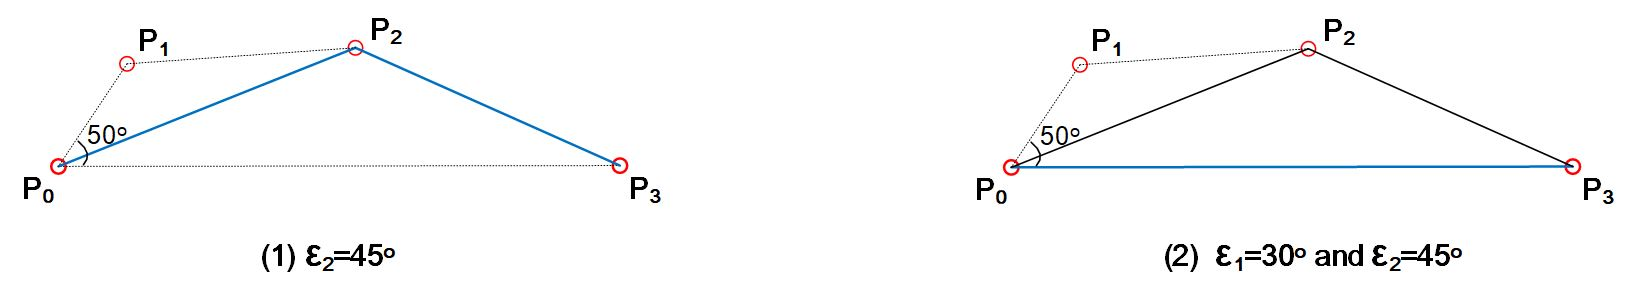
\includegraphics[scale=0.68]{Figures/Fig-aging-opt.jpg}
		
		\caption{\small A counter example of the aging friendliness of algorithm \opt using \dad, where (1) the original trajectory $\{P_0, P_1, P_2, P_3\}$ is compressed using $\epsilon_2=45^o$ to three points $\{P_0, P_2, P_3\}$, and (2) it is first compressed using $\epsilon_1=30^o$ to three points $\{P_0, P_2, P_3\}$, then compressed using $\epsilon_2=45^o$ to two points $\{P_0, P_3\}$. }
		\vspace{-1ex}
		\label{fig:aging-opt-dad}
\end{figure}

%%%%%%%%%%%%%%%%%%%%%%%% DP + DAD

\begin{proposition}
	\label{theo-aging-dp-dad}
	The top-down algorithm \dpa is not aging friendly \wrt~\dad.
\end{proposition}

\begin{proof}
	We shall prove this by constructing a counter-example shown in Figure~\ref{fig:aging-dp-dad}, where error bounds $\epsilon_1 =30^o$ and $\epsilon_2=45^o$.
	
	\underline{(1) ${\dpa}(\dddot{\mathcal{T}}, 45^o, \dad)$}. It finds that line segment $\overline{P_1P_2}$ has the largest angular deviation to line segment $\overline{P_0P_4}$ which is also larger than the error bound $45^o$, hence it uses point $P_2$ as the splitting point and splits the original trajectory to $\{P_0, P_1, P_2\}$ and $\{P_2, P_3, P_4\}$. At last, it outputs three points $\{P_0, P_2, P_4\}$.
	
	\underline{(2) ${\dpa}(\dpa(\dddot{\mathcal{T}}, 30^o, \dad), 45^o, \dad)$}. In the first round ($\epsilon_1=30^o$), the original trajectory is compressed to three points $\{P_0, P_2, P_4\}$, and in the second round ($\epsilon_2=45^o$), because line segments  $\overline{P_0P_2}$ and $\overline{P_2P_4}$ both have angular deviations to line segment $\overline{P_0P_4}$ less than $45^o$, it is finally compressed to two points $\{P_0, P_4\}$.
	
	In this case, ${\dpa}(\dddot{\mathcal{T}}, 45^o, \dad) \ne {\dpa}(\dpa(\dddot{\mathcal{T}}, 30^o, \dad), 45^o, \dad)$. Thus, the \dpa algorithm is not aging friendly \wrt~\dad.
\end{proof}

\begin{figure}
	\centering
	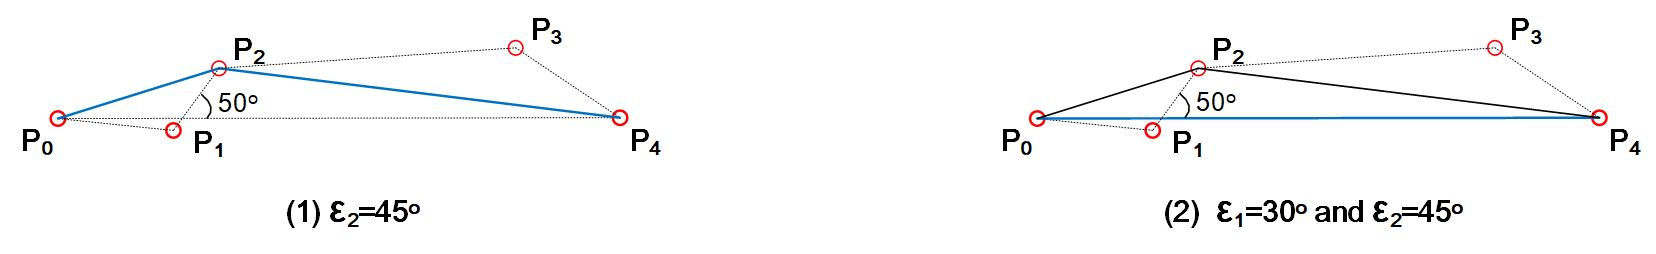
\includegraphics[scale=0.66]{Figures/Fig-aging-dp.jpg}
	
	\caption{\small A counter example of the aging friendliness of \dpa using \dad, where (1) the original trajectory is compressed using $\epsilon_2=45^o$ to three points $\{P_0, P_2, P_4\}$, and (2) the original trajectory is first compressed using $\epsilon_1=30^o$ to three points $\{P_0, P_2, P_4\}$, then compressed using $\epsilon_2=45^o$ to two points $\{P_0, P_4\}$. }
	\vspace{-1ex}
	\label{fig:aging-dp-dad}
\end{figure}

The \dpa using \dad is different with \ped and \sed in that \dad is the deviation between two line segments rather than the deviation between a point and a line segment. For example, in Figure \ref{fig:aging-dp-dad}-(2), the angular deviations of line segments $\overline{P_1P_2}$ and $\overline{P_0P_2}$ to line segment $\overline{P_0P_4}$ are certainly different though they pass through the same point $P_2$, thus, in the first round of run ($\epsilon_1=30^o$), the point $P_2$ serves as a splitting point while in the second round of run ($\epsilon_2=45^o$), it is no more a splitting point. This difference is the key that lets \dpa using \dad not aging friendly.
%
We next discuss the aging friendliness of other algorithms.

\begin{figure}
	\centering
	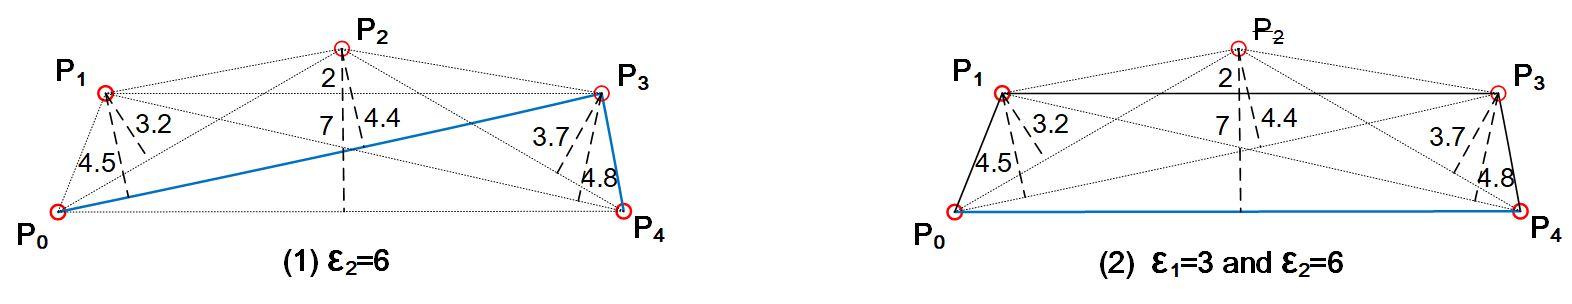
\includegraphics[scale=0.66]{Figures/Fig-aging-pavlidis.jpg}

	\caption{\small A counter example of the aging friendliness of algorithm \tpa, where (1) the original trajectory is compressed using $\epsilon_2=6$ to three points $\{P_0, P_3, P_4\}$, and (2) the original trajectory is first compressed using $\epsilon_1=3$ to four points $\{P_0, P_1, P_3, P_4\}$, then compressed using $\epsilon_2=6$ to two points $\{P_0, P_4\}$. }
	\vspace{-1ex}
	\label{fig:aging-pavlidis}
\end{figure}


\begin{proposition}
\label{theo-aging-tp}
The bottom-up algorithm \tpa is not aging friendly \wrt~\ped, \sed or \dad.
\end{proposition}

\begin{proof}
	We shall prove this by constructing a counter-example shown in Figure~\ref{fig:aging-pavlidis}, where error bounds $\epsilon_1 =3$ and $\epsilon_2=6$, and without losing generality, we use \ped as the distance metric.

\underline{(1) ${\tpa}(\dddot{\mathcal{T}}, 6, \ped)$}. It first merges $\overline{P_1P_2}$ and $\overline{P_2P_3}$ to $\overline{P_1P_3}$ as the merging of them has the lowest cost of $2$, the distance from point $P_2$ to line segment $\overline{P_1P_3}$; then it merges $\overline{P_0P_1}$ and $\overline{P_1P_3}$ to $\overline{P_0P_3}$ with the lowest cost of $4.5$, the distance from point $P_1$ to line segment $\overline{P_0P_3}$; at last, because the merging of $\overline{P_0P_3}$ and $\overline{P_3P_4}$ has a cost of $7$, the distance from point $P_2$ to line segment $\overline{P_0P_4}$, which is larger than the error bound of $6$, it outputs three points $\{P_0, P_3, P_4\}$.

\underline{(2) ${\tpa}(\tpa(\dddot{\mathcal{T}}, 3, \ped), 6, \ped)$}. In the first round ($\epsilon_1=3$), the original trajectory is compressed to four points $\{P_0, P_1, P_3, P_4\}$, and in the second round ($\epsilon_2=6$), because all points in the result trajectory $\{P_0, P_1, P_3, P_4\}$ have distances to line segment $\overline{P_0P_4}$ less than $6$, it is finally compressed to two points $\{P_0, P_4\}$.

In this case, ${\tpa}(\dddot{\mathcal{T}}, 6, \ped) \ne {\tpa}(\tpa(\dddot{\mathcal{T}}, 3, \ped), 6, \ped)$. Thus, \tpa is not aging friendly \wrt~\ped.
Similarly, \tpa is not aging friendly \wrt~ \sed or \dad. Hence, we have the conclusion.
\end{proof}


\eat{%%%%%%%%%%%%%
\begin{proposition}
	\label{theo-aging-squishe}
	The online algorithm \squishe is not aging friendly \wrt~\sed.
\end{proposition}

\begin{proof}
	{(In brief) The \squishe algorithm runs in a bottom-up manner that is a slight variation of algorithm \tpa. As \tpa, it is not aging friendly \wrt~\sed.}
\end{proof}
}%%%%%%%%%%%%%%%%
	
\begin{figure}[tb!]
	\centering
	\includegraphics[scale=0.66]{Figures/Fig-aging-incre.jpg}
	\vspace{-1ex}
	\caption{\small Counter examples of the aging friendliness of incremental algorithms (either online or one-pass).}
	\vspace{-1ex}
	\label{fig:aging-incre}
\end{figure}

\begin{proposition}
	\label{theo-aging-online}
	The online and one-pass algorithms are not aging friendly \wrt \ped, \sed or \dad.

\end{proposition}

\begin{proof}
	For online algorithm \squishe, it supports \sed only and runs in a bottom-up manner that is a slight variation of algorithm \tpa. As \tpa, it is not aging friendly \wrt~\sed.
	For other online and one-pass algorithms, though they apply different distance checking approaches, they run in a common incremental manner, \ie they incrementally read data points until they can not represent those read points by one line segment, then they output the simplified sub-trajectory and continue to process the rest data points. We next construct counter examples to show that an incremental algorithm $\mathcal{A}$ is not aging friendly.
	
	\underline{(1) ${\mathcal{A}}(\dddot{\mathcal{T}}, \epsilon_2, \mathcal{M})$}. As shown in Figure~\ref{fig:aging-incre}-(1)(3)(5), the algorithm $\mathcal{A}$ incrementally reads $\{P_0, P_1,\dddot, P_5\}$ and finds they can be represented by line segment $\overline{P_0P_4}$, thus the process progresses. Then, after point $P_6$ is read, it finds that these points can not be represented by any line segment, hence $\overline{P_0P_5}$ is output. Finally, the algorithm outputs $\{P_0, P_5, P_6\}$.
	
	\underline{(2) ${\mathcal{A}}(\mathcal{A}(\dddot{\mathcal{T}}, \epsilon_1, \mathcal{M}), \epsilon_2, \mathcal{M})$}. When using $\epsilon_1=4$ or $\epsilon_1=30^o $, the algorithm also outputs $\{P_0, P_5, P_6\}$. Then $\{P_0, P_5, P_6\}$ is compressed using $\epsilon_2=6$ or $\epsilon_2=45^o$ to $\{P_0, P_6\}$, as shown in Figure~\ref{fig:aging-incre}-(2)(4)(6).
	
	Combining (1) with (2), it is clear that the incremental algorithms are not aging friendly \wrt~distance metric \ped, \sed or \dad.
\end{proof}


{Though \dpa (using either \ped or \sed) is the only algorithm with the aging friendly feature, it is not necessarily the only algorithm that we have to use for compressing trajectories. Indeed, all the other algorithms are also applicable to compress trajectories in data aging although these algorithms may lead to (a bit) poorer compression ratios compared with \dpa. However, compression ratios are only one aspect of qualities for line simplification algorithms. Further, to keep aging friendliness, each run of algorithm \dpa must take as input the entire original or simplified trajectory that has the same start and end data points, and is not aging friendly, otherwise.}


\subsection{{Error} of Data Aging}
\label{sec-aging-safe}
As most algorithms are not aging friendly, are they error bounded in data aging?
if so, what are the bounds?
This section focuses on these problems and discusses the error between the simplified trajectory $\overline{\mathcal{T}}_2$ and the original trajectory $\dddot{\mathcal{T}_0}$.

%\stitle{{Aging safe}}. {Let $\mathcal{A}$ be a line simplification algorithm,  $\mathcal{M}$ be a distance metric, and $\epsilon_1>0$ and $\epsilon_2>0$ be error bounds, algorithm $\mathcal{A}$ is \emph{aging safe} if the errors between original trajectory $\dddot{\mathcal{T}}$ and simplified trajectory $\overline{\mathcal{T}}=\mathcal{A}(\mathcal{A}(\dddot{\mathcal{T}}, \epsilon_1, \mathcal{M}), \epsilon_2, \mathcal{M})$ are not more than $\epsilon_1+ \epsilon_2$. }


\begin{proposition}
	\label{theo-aging-error-dp}
	Given error bounds $\epsilon_1>0$ and $\epsilon_2>0$, for distance metric $\mathcal{M}$ of \ped and \sed, the error bound between the original trajectory $\dddot{\mathcal{T}}$ and simplified trajectory $\overline{\mathcal{T}}=DP(DP(\dddot{\mathcal{T}}, \epsilon_1, \mathcal{M}), \epsilon_2, \mathcal{M})$ is $max(\epsilon_1, \epsilon_2)$.
\end{proposition}

\begin{proof} We consider two cases: $\epsilon_2 \ge \epsilon_1$ and $\epsilon_2 < \epsilon_1$.

(1) For $\epsilon_2 \ge \epsilon_1$, as proved in \cite{Cao:Spatio}, $DP(DP(\dddot{\mathcal{T}}, \epsilon_1, \mathcal{M}), \epsilon_2, \mathcal{M}) = DP(\dddot{\mathcal{T}}, \epsilon_2, \mathcal{M})$, which has the max error of $\epsilon_2$ to the original trajectory $\dddot{\mathcal{T}}$.
	
(2) For $\epsilon_2 < \epsilon_1$, we shall prove $DP(DP(\dddot{\mathcal{T}}, \epsilon_1, \mathcal{M}), \epsilon_2, \mathcal{M}) = DP(\dddot{\mathcal{T}}, \epsilon_1, \mathcal{M})$ by  induction on the number of points of \trajec{T}.
\bi	
	\item  For a trajectory \trajec{T} with one or two points ($n=1$ or $n=2$), the simplified trajectories with any $\epsilon$ are sure identical to the original trajectory.
	Consider a trajectory \trajec{T} =	$[P_0, P_1, P_2]$ ($n = 3$),
	if the distance from $P_1$ to $\overline{P_0P_2}$ is less than $\epsilon_1$, then $DP(\dddot{\mathcal{T}}, \epsilon_1, \mathcal{M}) = [P_0, P_2]$. Obviously $DP(DP(\dddot{\mathcal{T}}, \epsilon_1, \mathcal{M}), \epsilon_2, \mathcal{M}))$ is $[P_0, P_2]$ too;	
	if the distance from $P_1$ to $\overline{P_0P_2}$ is larger than $\epsilon_1$, then $DP(\dddot{\mathcal{T}}, \epsilon_1, \mathcal{M})=\dddot{\mathcal{T}}$, and $DP(DP(\dddot{\mathcal{T}}, \epsilon_1, \mathcal{M}), \epsilon_2, \mathcal{M}) = DP(\dddot{\mathcal{T}}, \epsilon_2, \mathcal{M})=\dddot{\mathcal{T}}$.
	
	\item Assume that it is true for every trajectory \trajec{T} having $n \ge 3$ points.
	Consider a trajectory with $n+1$ points. Let $d_{max}$ denote the maximum distance between point $P_i$, $i \in [0,n]$, and the line segment $\overline{P_0P_{n}}$.
	If $d_{max}<\epsilon_1$, then $DP(\dddot{\mathcal{T}}, \epsilon_1, \mathcal{M})=[P_0, P_{n}]$, and $DP(DP(\dddot{\mathcal{T}}, \epsilon_1, \mathcal{M}), \epsilon_2, \mathcal{M}) = DP([P_0, P_{n}], \epsilon_2, \mathcal{M})=[P_0, P_{n}]$.
	If $d_{max} > \epsilon_1$, then in $DP(\dddot{\mathcal{T}}, \epsilon_1, \mathcal{M})$, point $P_i$ will split the trajectory \trajec{T} into two sub-trajectories, \ie $[P_0, ..., P_i]$ and $[P_{i}, ..., P_{n}]$, and continue to simplify each sub-trajectory. Hence, the result of $DP(\dddot{\mathcal{T}}, \epsilon_1, \mathcal{M})$ is the union of $DP([P_0, ..., P_i], \epsilon_1, \mathcal{M})$ and $DP([P_i, ..., P_n], \epsilon_1, \mathcal{M})$.
	Obviously, the points $P_0$, $P_i$ and $P_n$ are in the simplified trajectory of $DP(\dddot{\mathcal{T}}, \epsilon_1, \mathcal{M})$, and $P_i$ is still the first splitting point of the \dpa algorithm taking the simplified trajectory and $\epsilon_2$ as input. Hence, $DP(DP(\dddot{\mathcal{T}}, \epsilon_1, \mathcal{M}), \epsilon_2, \mathcal{M})$ is the union of $DP(DP([P_0, ..., P_i], \epsilon_1, \mathcal{M}), \epsilon_2, \mathcal{M})$ and $DP(DP([P_i, ..., P_n], \epsilon_1, \mathcal{M}), \epsilon_2, \mathcal{M})$. By the assumption, we have $DP(DP([P_0, ..., P_i], \epsilon_1, \mathcal{M}), \epsilon_2, \mathcal{M}) = DP([P_0, ..., P_i], \epsilon_1, \mathcal{M})$ and $DP(DP([P_i, ..., P_n], \epsilon_1, \mathcal{M}), \epsilon_2, \mathcal{M}) = DP([P_i, ..., P_n], \epsilon_1, \mathcal{M})$. Thus, $DP(DP(\dddot{\mathcal{T}}, \epsilon_1,$ $\mathcal{M}), \epsilon_2, \mathcal{M}) = DP(\dddot{\mathcal{T}}, \epsilon_1, \mathcal{M})$.

\item  Now we have $DP(DP(\dddot{\mathcal{T}}, \epsilon_1, \mathcal{M}), \epsilon_2, \mathcal{M}) = DP(\dddot{\mathcal{T}}, \epsilon_1, \mathcal{M})$, whose max error to the original trajectory $\dddot{\mathcal{T}}$ is $\epsilon_1$.
\ei

Combining (1) with (2), we have the conclusion.
\end{proof}


\begin{proposition}
	\label{theo-aging-distance}
	Given error bounds $\epsilon_1>0$ and $\epsilon_2>0$, for any \lsa algorithm $\mathcal{A}$ and distance metric $\mathcal{M}$ of \ped, \sed and \dad other than \dpa using \ped and \sed, the error bound between the original trajectory $\dddot{\mathcal{T}}$ and simplified trajectory $\overline{\mathcal{T}}=\mathcal{A}(\mathcal{A}(\dddot{\mathcal{T}}, \epsilon_1, \mathcal{M}), \epsilon_2, \mathcal{M})$ is $\epsilon_1+ \epsilon_2$.
\end{proposition}

\begin{proof} 	We shall prove this by showing that the error bound is neither more than $\epsilon_1+ \epsilon_2$  nor less than $\epsilon_1+ \epsilon_2$,
from which we have that the error bound is exactly $\epsilon_1+ \epsilon_2$.

	(1) We first prove that the error bound is not more than $\epsilon_1+ \epsilon_2$. Suppose that a point $P_k$ is represented by line segment $\overline{P_iP_j}$ with error bound $\epsilon_1$, and points $P_i$ and $P_j$ are further represented by line segment $\overline{P_sP_t}$ with error bound $\epsilon_2$ (Figure~\ref{fig:aging-error}).
	If the distance metric is \ped, then the distance from $P'_k$ to $\overline{P_sP_t}$ is less than $\epsilon_2$, hence, the distance from $P_k$ to $\overline{P_sP_t}$ is less than $\epsilon_1 + \epsilon_2$.
	If it is \sed, then $|P_iP''_i|<\epsilon_2$, $|P_jP''_j|<\epsilon_2$, and $\frac{|P_iP'_k|}{|P'_kP_j|} = \frac{|P''_iP''_k|}{|P''_kP''_j|}$, hence, $|P'_kP''_k|<\epsilon_2$, and the distance from $P_k$ to $\overline{P_sP_t}$, \ie $|P_kP''_k|$, is less than $\epsilon_1 + \epsilon_2$.
	If it is \dad, then obviously the error between $\overline{P_kP_{k+1}}$ and $\overline{P_sP_t}$ is not more than $\epsilon_1+ \epsilon_2$.
	
	(2) We then prove that the  error bound is not less than $\epsilon_1+ \epsilon_2$.
	If $\mathcal{A}$ is a top-down algorithm using \dad, then from Figure~\ref{fig:aging-dp-dad}-(2) we can find that the error from $\overline{P_3P_4}$ to $\overline{P_0P_4}$ is $\angle{P_3P_4P_0} = \angle{P_3P_4P_2} + \angle{P_2P_4P_0}$, whose bound is not less than $\epsilon_1 + \epsilon_2$, thus the error bound between the original trajectory $\dddot{\mathcal{T}}$ and simplified trajectory $\overline{\mathcal{T}}=\mathcal{A}(\mathcal{A}(\dddot{\mathcal{T}}, \epsilon_1, \mathcal{M}), \epsilon_2, \mathcal{M})$ is not less than $\epsilon_1+ \epsilon_2$.
	If $\mathcal{A}$ is a bottom-up or incremental algorithm, either online or one-pass, then from Figure~\ref{fig:aging-pavlidis}-(2) or Figure~\ref{fig:aging-incre} we also have the conclusion.
	
	
	Combining (1) with (2), we have the conclusion.
\end{proof}

\begin{figure}[tb!]
	\centering
	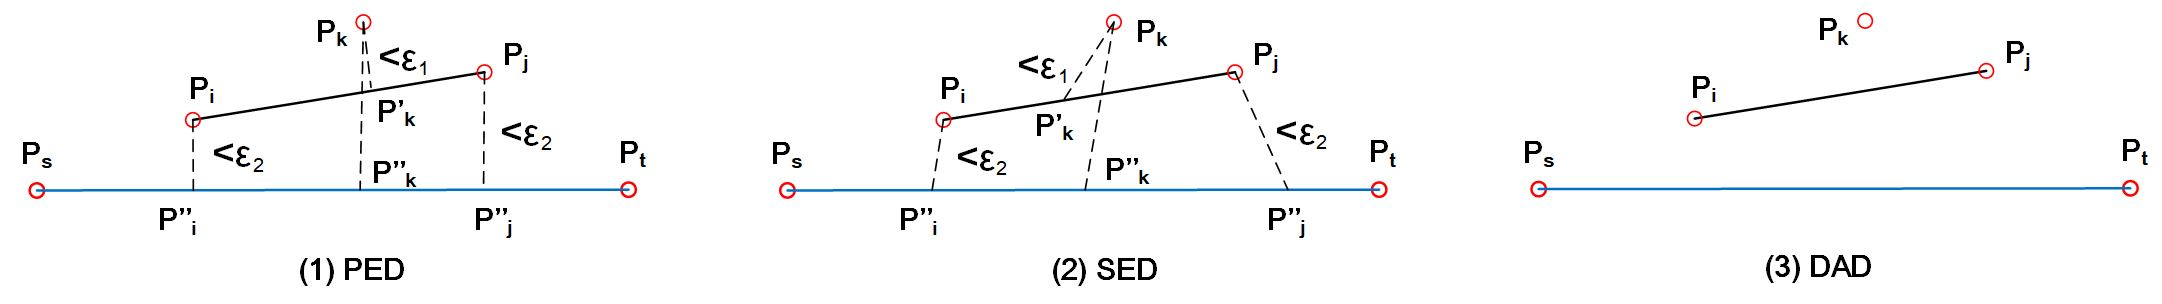
\includegraphics[scale=0.6]{Figures/Fig-aging-error.jpg}
	
	\caption{\small Examples of aging errors.}
	\vspace{-2ex}
	\label{fig:aging-error}
\end{figure}

{By Propositions \ref{theo-aging-error-dp} and \ref{theo-aging-distance}, it is obvious that all the above algorithms have bounded errors in data aging,  which make us freely re-compress trajectories by any of these algorithms as long as we use the same distance metric.}}

%%%%%%%%%%%%%%%%%%%%%%%%%%%%%%%%%%%%%%%%%%%%%%%%%%%%%%%%%%%%%%%%%%%%%%%%%%%%%%
%\vspace{-1ex}
\section{Evaluation} %Experimental Study
\label{sec-exp}
%%%%%%%%%%%%%%%%%%%%%%%%%%%%%%%%%%%%%%%%%%%%%%%%%%%%%%%%%%%%%%%%%%%%%%%%%%%%%%
In this section, we present extensive and systematic experimental studies and analyses of twelve representative \lsa algorithms.
Using three real-life datasets, we conduct five sets of tests to evaluate the effectiveness in terms of compression ratios and errors, efficiency (running time), data aging and query friendliness of these representative algorithms using distance metrics \ped, \sed and \dad, and the impacts of error bounds $\epsilon$ and trajectory sizes.
%
%(1) the effectiveness of these algorithms, and
%(2) the efficiency of them.
%{An additional test of the effectiveness of near optimal algorithm (\nopts) is presented in Appendix B.}

%\vspace{-1ex}
\subsection{Experimental Setting}
%We first introduce the settings of our experimental study.

\stitle{Real-life Trajectory Datasets}.
We use three real-life datasets shown in \mytable{tab:datasets}, namely, Service car trajectory data (\ucar), Geolife trajectory data (\geolife)~\cite{Web:Geolife} and \mopsi trajectory data (\mopsi)~\cite{Web:Mopsi}, to evaluate those \lsa algorithms.
These data sets come from different sources, where \ucar is collected by cars in urban, and \geolife and \mopsi are a mixing of cars and individuals. They also have {typical sampling rates used in practice, ranging from one point per second to one point per five seconds.}
\myblue{Occasionally, the time interval between two neighbouring data points is very long, \eg greater than $10^7$ seconds.}
The data source and sampling rate also affect the performance of \lsa algorithms using certain distance metrics.

%\vspace{0.5ex}
\ni {(1) \ucar is the GPS trajectories collected by a Chinese car rental company during Apr. 2015 to Nov. 2015. Most routes are located in big cities. The sampling rate is one point per $3$--$5$ seconds, and each trajectory has around $114.1K$ points.}
%.We randomly chose $1,000$ cars from them

%\vspace{0.5ex}
\ni {(2) \geolife is the GPS trajectories collected in the GeoLife project~\cite{Web:Geolife} by 182 users in a period from Apr. 2007 to Oct. 2011. These trajectories have a variety of sampling rates, among which 91\% are logged at one  point  per 1-5 seconds. The longest trajectory has 2,156,994 points.}

%\vspace{0.5ex}
\ni {(3) \mopsi is the GPS trajectories collected in the Mopsi project~\cite{Web:Mopsi} by 51 users in a period from 2008 to 2014. Most routes are located in Joensuu region, Finland. The sampling rate is one point per $2$ seconds, and each trajectory has around $153.9K$ points.}


\begin{table}[tb!]
	%\vspace{-1ex}
	\caption{\small Real-life trajectory datasets}
	\centering
	%\small
	\footnotesize
	\begin{tabular}{|l|c|c|c|c|}
		\hline
		\bf{Data sets}& \bf{Number\ of Trajectories}     &\bf{Sampling Rates (s)}   &\bf{Points~Per Trajectory}    &\bf{Total Points} \\	\hline
		%\taxi	&{500}	    &60	        &{$\sim42.8$K}      &{21.4M} \\	\hline
		%\truck	&10,368	    &1-60	    &$\sim71.9$     &746M \\	\hline
		%\ucar	&11,000	    &3-5	    &$\sim119.1$   &1.31G\\		\hline
		%
		\ucar	&\myblue{1000}	    &3-5	&$\sim114.0$K   &\myblue{114.0M} 	\\	\hline
		\geolife \cite{Web:Geolife}&182	    &1-5	&$\sim131.4$K   &24.2M	\\	\hline
		\mopsi \cite{Web:Mopsi}  &51	    	&2	    &$\sim153.9$K   &7.9M	\\	\hline
		%\act	& 10	    &1	    &$\sim11.8$    &112.8K	\\	\hline
	\end{tabular}
	\label{tab:datasets}
	\vspace{-2ex}
\end{table}


% \ni \emph{(1) Truck trajectory data} (\truck) is the GPS trajectories collected by \eat{10,368} trucks equipped with GPS sensors in China
% during a period from Mar. 2015 to Oct. 2015. The sampling rate varied from 1s to 60s.
%Trajectories mostly have around $50$ to $90$ thousand data points.



%\vspace{0.5ex}
%\ni \emph{(4) Act trajectory data} (\act) is a small set GPS trajectories collected with a high sampling rate of one point per second by our team members in 2017. There are 10 trajectories and each trajectory has around 11.8K points.

%The details of these datasets are shown in Table~\ref{tab:dataset}.

\stitle{Algorithms and implementation}.
We have implemented the representative algorithms shown in \mytable{tab:summary-lsa}.
 They are optimal algorithm \opt, batch algorithms \dpa and \tpa, online algorithms  \opwa, \bqsa, \squishe and \myblue{\dagots}, and one-pass algorithms  \operb, \siped, \cised, \intersec and \interval.
For one-pass algorithms \siped and \cised, we implement two versions of them (half and full $\epsilon$), denoted as \siped($\epsilon$), \siped($\frac{\epsilon}{2}$), \cised($\epsilon$) and \cised($\frac{\epsilon}{2}$). 
%\textcolor{blue}{The above algorithms all belong to strong simplification that output data points belong to the original trajectories.}
\textcolor{blue}{Besides, algorithms \operb\cite{Lin:Operb} and \cised\cite{Lin:Cised} both have weak versions, named \operb-A and \cised-W, that allow data interpolation. } %We also implement them.
For algorithm \cised($\epsilon$) and \cised($\frac{\epsilon}{2}$), we fixed parameter $m=16$ as evaluated in \cite{Lin:Cised}, \ie 16-edges inscribe regular polygon.
{For algorithm \operb, we remove its fifth optimization technique to make it fit for the definition of \textcolor{blue}{\emph{tolerance-zone} error measure \cite{Daescu:metric,Barequet:3D,Chen:Space,Imai:Optimal,Melkman:Optimal} (otherwise, it is the \emph{infinite beam} error measure \cite{Daescu:metric,Chen:Space})}.}
% For algorithm \nopts, we fixed parameter $m=32$.
All algorithms are implemented with Java.
{All tests are run on an x64-based  PC with 4 Intel(R) Core(TM) {i7-6700 CPU @3.40GHz} and 8GB of memory, and {the max heap size of Java VM is 4GB.}}
%, and each test was repeated over 3 times and the average is reported here.


We test these algorithms under varied error bounds $\epsilon$ and trajectory sizes, respectively. We first vary $\epsilon$ from $10m$ to $100m$ in \ped and \sed (or from $15^o$ to $90^o$ in \dad) on the entire four datasets, respectively. We then choose $10$ trajectories from each dataset, and vary the size \trajec{|T|} of a trajectory from $1,000$ points to $10,000$ points \textcolor{blue}{(\ie from top $1,000$ to top $10,000$ points of the trajectory)} while fixing the error bound $\epsilon=40$ metres or $\epsilon=45$ degrees.

\eat{%%%%%%%%%%%%%%%%%%%
	\stitle{Real-life Trajectory Datasets}.
	We use four real-life datasets shown in Table~\ref{tab:dataset} to test our solutions.
	
	\sstab{\bf(1) Taxi trajectory data}, referred to as \taxi, is the GPS trajectories collected by $12,727$ taxies equipped with GPS sensors in Beijing during a period
	from Nov. 1, 2010 to Nov. 30, 2010. The sampling rate was one point  per 60s, and \taxi has $39,100$ data points on average per trajectory.
	
	\sstab{\bf(2) Truck trajectory data}, referred to as \truck, is the GPS trajectories collected by 10,368 trucks equipped with GPS sensors in China
	during a period from Mar. 2015 to Oct. 2015. The sampling rate varied from 1s to 60s. Trajectories mostly have around $50$ to $90$ thousand data points.
	
	\sstab{\bf(3) Service car trajectory data}, referred to as \ucar,  is the GPS trajectories collected by a car rental company.
	We chose $11,000$ cars from them, during Apr. 2015 to Nov. 2015. The sampling rate was one point per $3$--$5$ seconds, and
	each trajectory has around $119.1K$ data points.
	
	{\sstab{\bf(4) GeoLife trajectory data}, referred to as \geolife, is the GPS trajectories collected in GeoLife project~\cite{Zheng:GeoLife} by 182 users in a period from Apr. 2007 to Oct. 2011. These trajectories have a variety of sampling rates, among which 91\% are logged in each 1-5 seconds or each 5-10 meters per point. The longest trajectory has 2,156,994 points.}
	%This dataset contains 182 trajectories, one trajectory for each user, with a total distance of about 1.2 million kilometers.
}%%%%%%%%%%%%%%%%%%%%%%%%%%%%%%%%%%%%%%%%%%%%%%%%%%%%%%%%%%%%%



\subsection{Evaluation Metrics}

{Compression ratios and errors are the most popular metrics to evaluate the effectiveness of \lsa algorithms, and they are also the measures to evaluate the aging friendliness of \lsa algorithms.
And the running time  is used to evaluate the efficiency of \lsa algorithms.}

\stitle{Compression ratios.}
For trajectories $\{\dddot{\mathcal{T}_1}, \ldots, \dddot{\mathcal{T}_M}\}$ and their piece-wise line representations $\{\overline{\mathcal{T}_1}, \ldots, \overline{\mathcal{T}_M}\}$,
the compression ratio is $(\sum_{j=1}^{M} |\overline{\mathcal{T}}_j |)/(\sum_{j=1}^{M} |\dddot{\mathcal{T}}_j |)$.
By this definition, algorithms with lower compression ratios are better.

\stitle{Simplification errors.}
\myblue{The max (or average) simplification error is the max (or average) value of the distances from every point of the original trajectories to its representing line segment of the simplified trajectories.}


\eat{
Given a set of trajectories $\{\dddot{\mathcal{T}_1}, \ldots, \dddot{\mathcal{T}_M}\}$ and their piece-wise line representations
$\{\overline{\mathcal{T}_1}, \ldots, \overline{\mathcal{T}_M}\}$, and $P_{j,i}$ denoting
\textcolor{blue}{one of the points} in trajectory $\dddot{\mathcal{T}}_j$ \textcolor{blue}{represented by} a line segment $\mathcal{L}_{l,i}\in\overline{\mathcal{T}_l}$ ($l\in[1,M]$), then {the max error is $max\{d(P_{j,i}, \mathcal{L}_{l,i})\}$ for each i,j, l in [1, M],} and the average error is $\sum_{j=1}^{M}\sum_{i=0}^{M} d(P_{j,i}, \mathcal{L}_{l,i})/\sum_{j=1}^{M}{|\dddot{\mathcal{T}}_j |}$.
\textcolor{blue}{Note that each point in the original trajectories are counted.}
\todo{Are the ranges of i,j, l correct?}}

\stitle{Running time.}
It is the efficiency of algorithms.
%We load and compress trajectories one by one, and only count the running time of the compressing process.


%%%%%%%%%%%%%%%%%%%%%%%%%%%%%%%%%%%%%%%%%%%%%%%%%%%%%%%%%%%%%%%%%%%%%%%%%%%%%%
\subsection{Experimental Results and Analyses}
%%%%%%%%%%%%%%%%%%%%%%%%%%%%%%%%%%%%%%%%%%%%%%%%%%%%%%%%%%%%%%%%%%%%%%%%%%%%%%
We next present our findings.




%%%%%%%%%%%%%%%%%%%%%%%%%%%%%%%%%%%%%%%%%%%%%%%%%%%%%%%%%%%%%%%%%%%%%%%%%%%%%
%\vspace{-1ex}
\subsubsection{Evaluation and Analyses of Compression Ratio}
%%%%%%%%%%%%%%%%%%%%%%%%%%%%%%%%%%%%%%%%%%%%%%%%%%%%%%%%%%%%%%%%%%%%%%%%

\eat{%%%%%%%
We first test the compression ratios of these algorithms under varied error bounds $\epsilon$ and trajectory sizes, respectively. We varied $\epsilon$ from $10m$ to $100m$ in \ped and \sed (or from $15^o$ to $90^o$ in \dad) on the entire four datasets, respectively. The results are reported in Figure~\ref{fig:cr-ped-epsilon}, Figure~\ref{fig:cr-sed-epsilon} and Figure~\ref{fig:cr-dad-epsilon} ({Note that the naive optimal algorithm using \sed or \dad is not reported here because it can not run with the full dataset as input}).
%
We then chose $10$ trajectories from each dataset \taxi, \ucar, \geolife and \mopsi, respectively, and varied the size \trajec{|T|} of a trajectory from $1,000$ points to $10,000$ points, while fixed error bound $\epsilon = 60$ meters for \ped and \sed ({or $\epsilon = 45$ degrees for \dad}).
The experimental results are reported in Figure~\ref{fig:cr-ped-size}, Figure~\ref{fig:cr-sed-size} and Figure~\ref{fig:cr-dad-size}.
}%%%%%%%%%%%

%We test the compression ratios of these algorithms under varied error bounds $\epsilon$ and trajectory sizes, respectively.
The compression ratios of these algorithms under varied error bounds $\epsilon$ and trajectory sizes are reported in Figures~\ref{fig:cr-ped-epsilon},~\ref{fig:cr-sed-epsilon},~\ref{fig:cr-dad-epsilon},~\ref{fig:cr-ped-size},~\ref{fig:cr-sed-size} and~\ref{fig:cr-dad-size}.
{Note that the optimal algorithm using \sed and \dad is not reported in Figures~\ref{fig:cr-ped-epsilon},~\ref{fig:cr-sed-epsilon} and~\ref{fig:cr-dad-epsilon} as it runs out of memory when compressing the full dataset}. We first report our findings.


%%%%%%%%%%%%%%%%%
\sstab(1)  {Datasets may have impacts on the compression ratios of \lsa algorithms. Datasets with higher sampling rates typically have better compression ratios for \ped and \sed, while it is opposite for \dad. \textcolor{blue}{When using \dad, the} dataset collected by cars (\eg~\ucar) has better compression ratios than the datasets partially collected by individuals (\eg~\geolife and \mopsi), as cars typically move more regularly than individuals \textcolor{blue}{in directions}. }

\sstab(2) \textcolor{blue}{Data sizes do not have remarkable impacts on compression ratios.}

\sstab(3) The compression ratios of algorithms using \ped from the best
to the worst are normally the optimal algorithm \opt, online algorithm \bqsa, one-pass algorithm \siped($\epsilon$), batch algorithms \tpa and \dpa and one-pass algorithm \myblue{\operb-A}, and one-pass algorithms \siped($\frac{\epsilon}{2}$) and \operb.
The output sizes of algorithms \bqsa and \siped({$\epsilon$}) are on average
($113.32\%$, $120.22\%$, $120.83\%$) and ($116.04\%$, $124.46\%$, $124.24\%$) of algorithm \opt
on datasets \dSets, respectively.
Algorithms \tpa, \dpa and \myblue{\operb-A} are comparable, and their output sizes are on average
($125.05\%$, $131.01\%$, $138.01\%$), ($130.03\%$, $140.56\%$, $139.00\%$) and \myblue{( $134.16\%$, $137.73\%$, $144.31\%$)} of \opt
on datasets \dSets, respectively.
Algorithms \siped($\frac{\epsilon}{2}$) and \operb are comparable, and they are on average
($136.73\%$, $150.23\%$, $152.29\%$) and ($143.14\%$, $147.80\%$, $152.37\%$) of \opt on datasets \dSets, respectively.
%
For example, in \mopsi, the compression ratios of algorithms
(\opt, \tpa, \dpa, \bqsa, \siped(${\epsilon}$), \siped($\frac{\epsilon}{2}$), \operb, \myblue{\operb-A} ) are ($1.6\%$, $2.2\%$, $2.2\%$, $1.9\%$, $2.0\%$, $2.4\%$, $2.4\%$, \myblue{$2.3\%$}) when $\epsilon$ = $40m$.
%


\begin{figure*}[tb!]
	\centering
	%\includegraphics[scale=0.250]{Figures/Exp-PED-CR-epsilon-taxi.jpg}\hspace{0.5ex}
	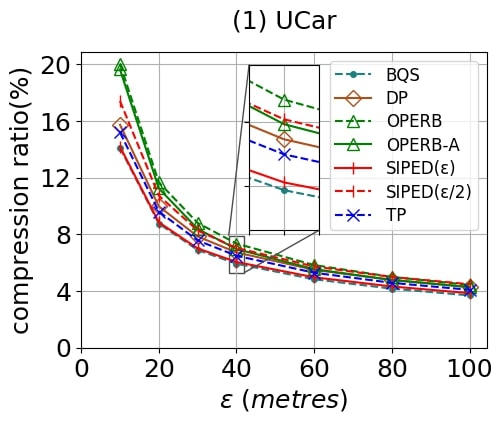
\includegraphics[scale=0.250]{Figures/Exp-PED-CR-epsilon-service.jpg} 	\hspace{0.5ex}
	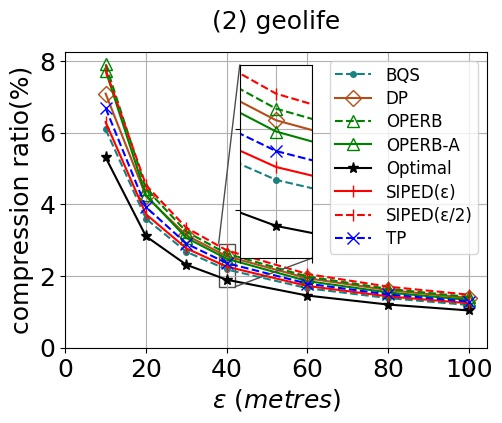
\includegraphics[scale=0.348]{Figures/Exp-PED-CR-epsilon-geolife.jpg}	\hspace{0.5ex}
	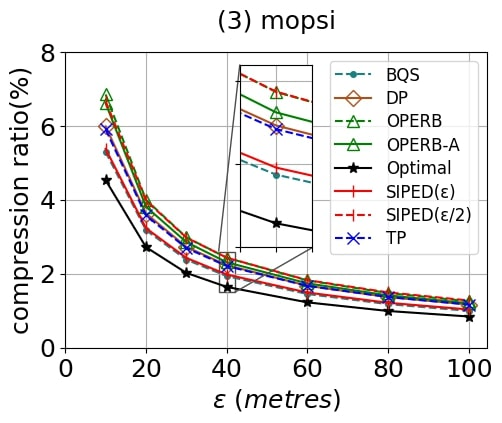
\includegraphics[scale=0.250]{Figures/Exp-PED-CR-epsilon-mopsi.jpg}		
	\vspace{-2ex}
	\caption{\small Evaluation of compression ratios (\ped) on full datasets: varying the error bound $\epsilon$.}
	\label{fig:cr-ped-epsilon}
	\vspace{-2ex}
\end{figure*}
\begin{figure*}[tb!]
	\centering
	%\includegraphics[scale=0.250]{Figures/Exp-SED-CR-epsilon-taxi.jpg}\hspace{0.5ex}
	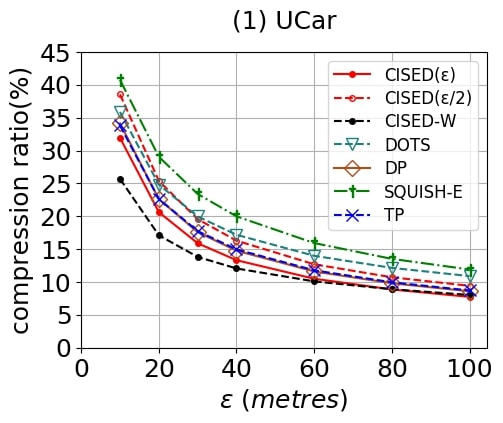
\includegraphics[scale=0.250]{Figures/Exp-SED-CR-epsilon-service.jpg} 	\hspace{0.5ex}
	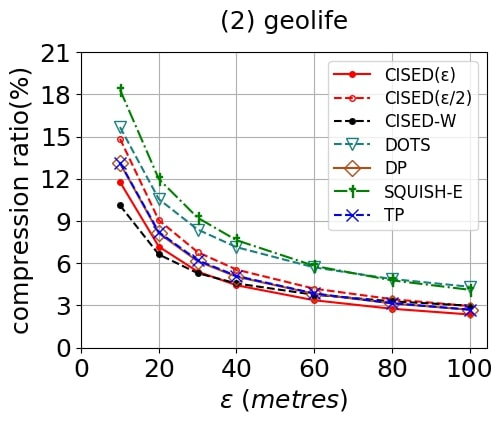
\includegraphics[scale=0.250]{Figures/Exp-SED-CR-epsilon-geolife.jpg}	\hspace{0.5ex}
	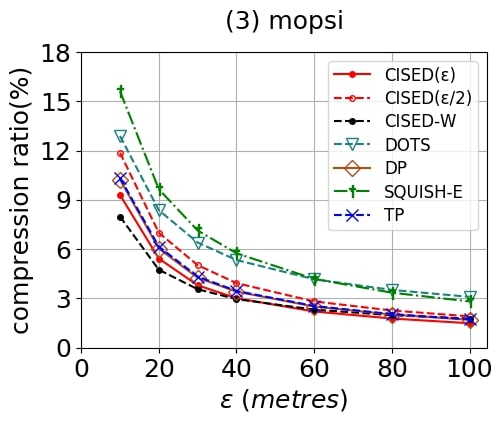
\includegraphics[scale=0.250]{Figures/Exp-SED-CR-epsilon-mopsi.jpg}		
	\vspace{-2ex}
	\caption{\small Evaluation of compression ratios (\sed) on full datasets: varying the error bound $\epsilon$.}
	\label{fig:cr-sed-epsilon}
	\vspace{-2ex}
\end{figure*}
\begin{figure*}[tb!]
	\centering
	%\includegraphics[scale=0.250]{Figures/Exp-DAD-CR-epsilon-taxi.jpg}\hspace{0.5ex}
	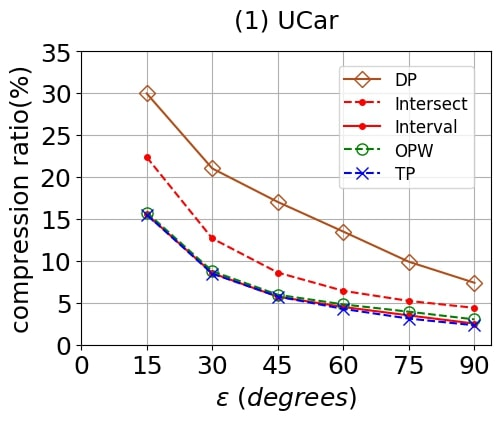
\includegraphics[scale=0.250]{Figures/Exp-DAD-CR-epsilon-service.jpg} 	\hspace{0.5ex}
	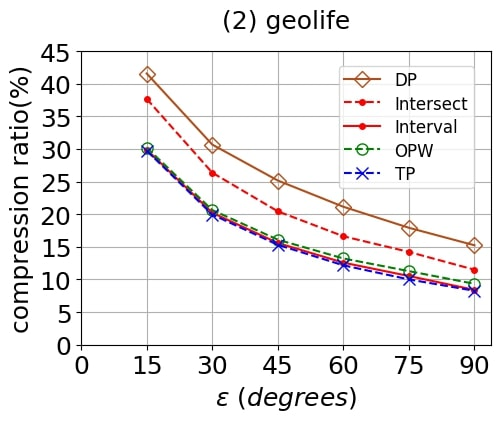
\includegraphics[scale=0.250]{Figures/Exp-DAD-CR-epsilon-geolife.jpg}	\hspace{0.5ex}
	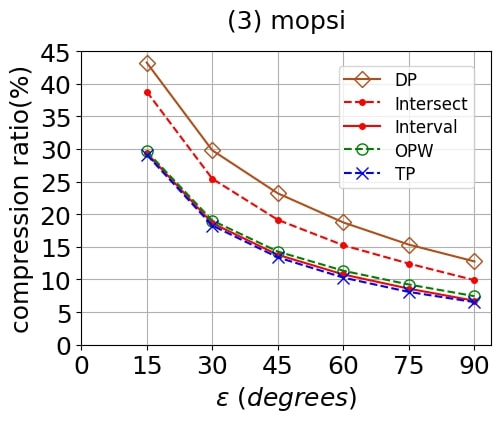
\includegraphics[scale=0.250]{Figures/Exp-DAD-CR-epsilon-mopsi.jpg}		
	\vspace{-2ex}
	\caption{\small Evaluation of compression ratios (\dad) on full datasets: varying the error bound $\epsilon$.}
	\label{fig:cr-dad-epsilon}
	\vspace{-2ex}
\end{figure*}

%%%%%%%%%%%%%%%%%
\sstab(4) The compression ratios of algorithms using \sed from the best
to the worst are normally the \opt algorithm, one-pass algorithms \myblue{\cised-W} and \cised($\epsilon$), batch algorithms \tpa and
\dpa, one-pass algorithm \cised($\frac{\epsilon}{2}$), and online algorithm {\dagots} and \squishe.
%
{Algorithms \tpa and \dpa are comparable, and they are on average
($125.23\%$, $143.92\%$, $128.63\%$) and ($123.93\%$, $141.46\%$, $121.14\%$)
 of algorithm \opt on datasets \dSets, respectively.}
%
{Algorithms \myblue{\cised-W}, \cised(${\epsilon}$), \cised($\frac{\epsilon}{2}$), \squishe and {\dagots} are on average \myblue{($100.98\%, 108.16\%, 110.15\%$)}, ($109.27\%$, $110.13\%$, $115.90\%$,), ($134.35\%$, $159.30\%$, $136.06\%$), ($165.94\%$, $225.68\%$, $206.90\%$) and \myblue{$(140.98\%, 200.36\%, 198.73\%)$}
 of \opt on \dSets, respectively.}
%
For example, in \mopsi, the compression ratios of algorithms
(\tpa, \dpa, \squishe, {\dagots}, \cised(${\epsilon}$), \cised($\frac{\epsilon}{2}$),  \myblue{\cised-W})
are ($3.45\%$, $3.41\%$, $5.75\%$, \myblue{$5.34\%$}, $3.02\%$, $3.86\%$,  \myblue{$2.96\%$}), respectively, when $\epsilon$ = $40m$.
%
%Algorithms \tpa and \dpa are comparable, and they are on average ($122.69\%$, $129.08\%$, $131.97\%$, $131.01\%$) and ($121.36\%$, $129.27\%$, $130.11\%$, $126.21\%$) of the near optimal algorithm \nopts on datasets \dSets, respectively.
%Algorithms \cised and \squishe are on average ($132.07\%$, $139.67\%$, $146.56\%$, $135.10\%$) and ($164.47\%$, $189.87\%$, $213.30\%$, $186.72\%$) of \nopts on datasets \dSets, respectively.
%
%For example, in \mopsi, the compression ratios of algorithms (\nopts, \tpa, \dpa, \squishe, \cised) are ($2.62\%$, $3.45\%$, $3.41\%$, $5.75\%$, $3.86\%$), respectively, when $\epsilon$ = $40m$.
%

%%%%%%%%%%%%%%%%%
\sstab(5) The compression ratios of algorithms using \dad from the best
to the worst are the \opt algorithm, batch algorithm \tpa and
one-pass algorithm \interval, online algorithm \opwa, one-pass algorithm \intersec and batch algorithm \dpa.
%
{Algorithms \tpa, \opwa and \interval are comparable, and are on average
($102.91\%$, $102.27\%$, $106.88\%$), ($116.09\%$, $107.11\%$, $115.42\%$) and ($101.98\%$, $103.52\%$, $103.43\%$)
 of algorithm \opt on datasets \dSets, respectively.}
%
{Algorithms \intersec and \dpa are on average ($156.00\%$, $121.20\%$, $230.52\%$) and ($283.93\%$, $143.79\%$, $278.89\%$)
 of algorithm \opt on datasets \dSets, respectively.}
%
For example, in \mopsi, the compression ratios of algorithms (\tpa, \dpa, \opwa, \interval, \intersec)
are ($13.3\%$, $23.1\%$, $14.12\%$, $13.7\%$, $18.96\%$), respectively, when $\epsilon$ = $45$ degrees.
%






We then present analyses from the views of \lsa algorithms and distance metrics.


\stitle{Analyses of \lsa algorithms}. The \opt algorithm is the best in terms of compression ratios, followed by online algorithms \opwa and \bqsa and one-pass algorithms using the full $\epsilon$ \emph{sector/cone/range}. One-pass algorithms using a half $\epsilon$ \emph{sector/cone/range} and batch algorithms except \dpa using \dad also have good compression ratios.
\eat{
 are the most outstanding algorithms among all sub optimal algorithms.
, followed by batch algorithms. Online algorithms have varied compression ratios, ranging from the worst to the similar with batch and one-pass algorithms.
}

\begin{figure*}[tb!]
	\centering
	%\includegraphics[scale=0.250]{Figures/Exp-PED-CR-size-taxi.jpg}\hspace{0.5ex}
	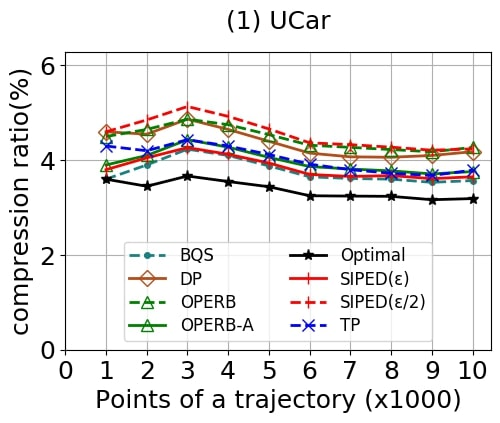
\includegraphics[scale=0.250]{Figures/Exp-PED-CR-size-service.jpg} 	\hspace{0.5ex}
	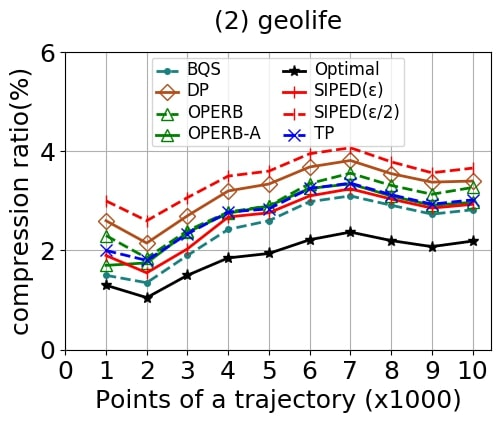
\includegraphics[scale=0.250]{Figures/Exp-PED-CR-size-geolife.jpg}	\hspace{0.5ex}
	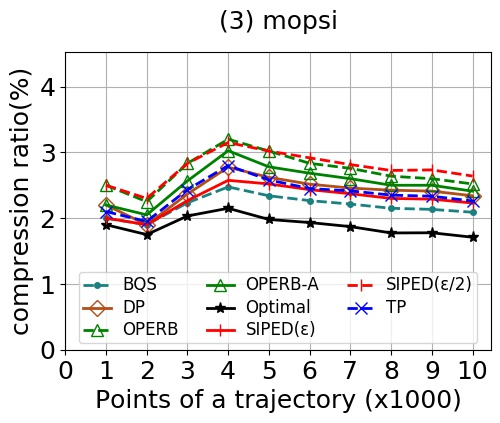
\includegraphics[scale=0.348]{Figures/Exp-PED-CR-size-mopsi.jpg}		
	\vspace{-2ex}
	\caption{\small Evaluation of compression ratios (\ped) on small datasets: varying the size of
		trajectories.}
	\label{fig:cr-ped-size}
	\vspace{-2ex}
\end{figure*}
\begin{figure*}[tb!]
	\centering
	%\includegraphics[scale=0.250]{Figures/Exp-SED-CR-size-taxi.jpg}\hspace{0.5ex}
	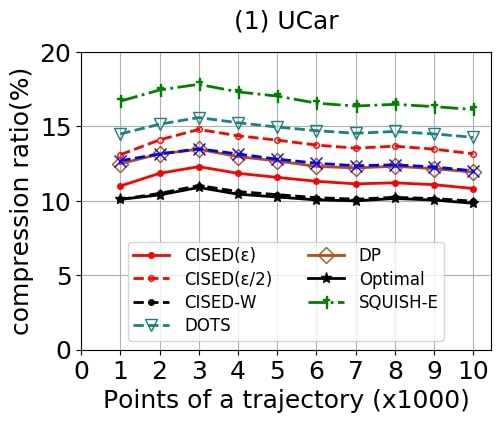
\includegraphics[scale=0.250]{Figures/Exp-SED-CR-size-service.jpg} 	\hspace{0.5ex}
	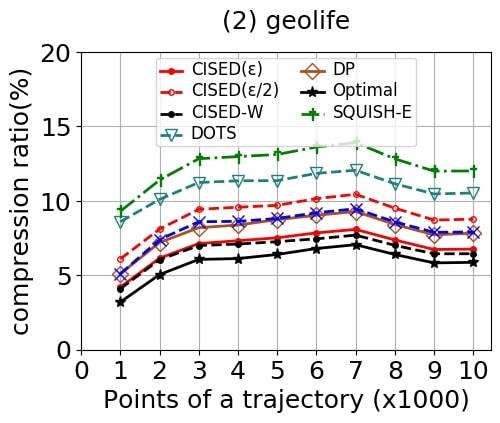
\includegraphics[scale=0.250]{Figures/Exp-SED-CR-size-geolife.jpg}	\hspace{0.5ex}
	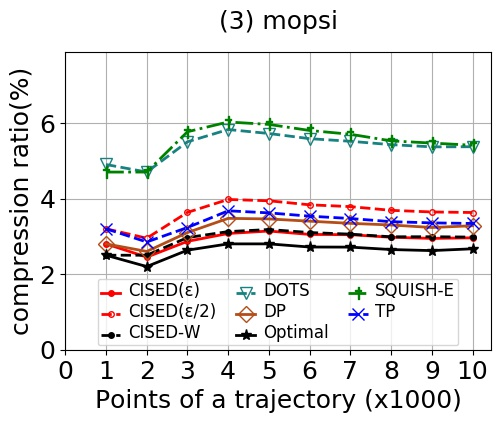
\includegraphics[scale=0.348]{Figures/Exp-SED-CR-size-mopsi.jpg}		
	\vspace{-2ex}
	
	\caption{\small Evaluation of compression ratios (\sed) on small datasets: varying the size of
		trajectories.}
	\label{fig:cr-sed-size}
	\vspace{-2ex}
\end{figure*}
\begin{figure*}[tb!]
	\centering
	%\includegraphics[scale=0.50]{Figures/Exp-DAD-CR-size-taxi.jpg}\hspace{0.5ex}
	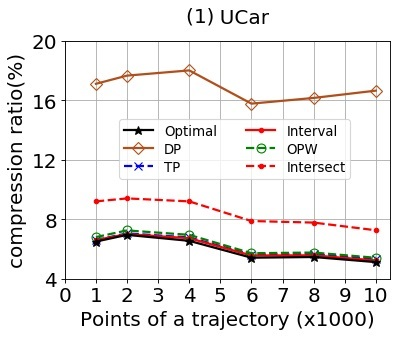
\includegraphics[scale=0.52]{Figures/Exp-DAD-CR-size-service.jpg} 	\hspace{0.5ex}
	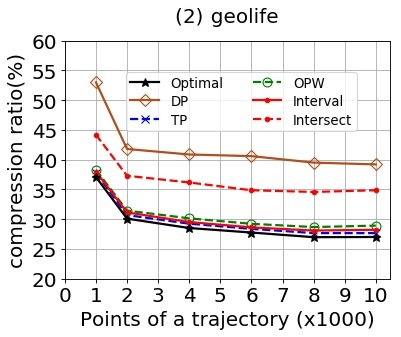
\includegraphics[scale=0.52]{Figures/Exp-DAD-CR-size-geolife.jpg}	\hspace{0.5ex}
	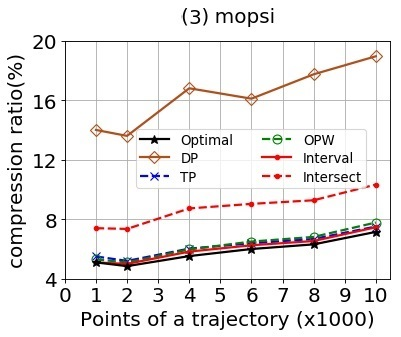
\includegraphics[scale=0.52]{Figures/Exp-DAD-CR-size-mopsi.jpg}		
	\vspace{-2ex}
	\caption{\small Evaluation of compression ratios (\dad) on small datasets: varying the size of trajectories.}
	\label{fig:cr-dad-size}
	\vspace{-2ex}
\end{figure*}


%\todo{Batch: Bottom-up vs Top-down.}
For batch algorithms, bottom-up algorithm (\tpa) and top-down algorithm (\dpa) have the similar compression ratios when using \ped and \sed. However, when using \dad, bottom-up methods have obviously better compression ratios than top-down methods.  As we know that top-down algorithms split a long trajectory $[P_s, ..., P_e]$ into two sub trajectories by finding out a splitting point $P_i (s<i<e)$ that has the max position deviation (or whose line segment $\vv{P_{i-1}P_{i}}$ has the max direction deviation) to line segment $\vv{P_sP_{e}}$. Though this strategy works well with \ped and \sed, a point with the max direction deviation may not be a reasonable splitting point in the direction-aware scenario. Thus it leads to a poorer compression ratio. However, bottom-up methods do not have this weakness as they always merge neighbouring points.



%\todo{Online: }
For online algorithms, \bqsa and \opwa are comparable with the best sub-optimal algorithms. This is because \opwa is indeed a combination of \dpa and opening window, and \bqsa is mainly an efficiency optimized \opwa.
\squishe has the poorest compression ratio among all algorithms using \sed. This is the result of its mechanism: \squishe estimates the lowest \sed error and removes the point with ``predicted to introduce the lowest amount of error into the compression"\cite{Muckell:SQUISH}. Its ``prediction" method is not accurate enough, thus, in order to ensure the error bound, it may ignore too many potential points that could be represented by a line segment. \textcolor{blue}{\dagots~also shows poor compression ratios in these tests. This is related to \lissed, a cumulative error measure that \dagots~uses, in which each point contributes a part of error, such that the \lissed error bound of $\epsilon^2$ may limit this algorithm to ``absorbing" more points into a line segment, even though those points could be absorbed \wrt the  \sed error bound of $\epsilon$.}

%\todo{One pass: half $\epsilon$ vs full $\epsilon$.}
For one-pass algorithms, the full $\epsilon$ sector/cone/range combining with a position/direction constraint always has better compression ratios than the half $\epsilon$ sector/cone/range versions in all datasets, and they are comparable with the best sub-optimal algorithms.
This may be related to the moving habits or patterns of moving objects that implied in trajectories.
That is, a moving object, like an individual or a car, usually keeps moving forward for quite a long time, engendering a sequence of data points distributing in a narrow strip. Under such circumstance, a new data point is quite possibly living in the common intersection of larger sectors/cones/ranges, which further leads to a better compression ratio. 
%which lets more data points be represented by a result line segment.

\textcolor{blue}{Besides, weak algorithms \operb-A and \cised-W normally have a few advantages in terms of compression ratios compared with corresponding strong algorithms \operb and \cised in cases that small error bounds (\eg $\epsilon<40$ meters in these tests) are set.}




\stitle{Analyses of distance metrics}.
Though \ped, \sed and \dad are different distances, the comparison of their compression ratios is helpful to choose an effective distance metric.
%whose usages are mainly decided by application requirements
%
First, \textcolor{blue}{because \sed saves temporal information while \ped does not (also note the loss of temporal information may lead to unexpected results, \eg unbounded answer-errors to spatio-temporal queries, see Section \ref{sec-exp-query})}, given the same error bound $\epsilon$, the compression ratios of algorithms using \ped are obviously better
than using \sed. More specifically, \emph{the output sizes of using \sed are approximately twice of \ped.}
%
As shown in Figures~\ref{fig:cr-ped-epsilon} and~\ref{fig:cr-sed-epsilon}, the output sizes of algorithms \tpa and \dpa
using \ped are on average ($43.55\%$, $47.49\%$, $63.15\%$) and ($45.79\%$,
$50.88\%$, $64.50\%$) of algorithms \tpa and \dpa using \sed on datasets \dSets, respectively.
%
%and in Figure~\ref{fig:cr-ped-size} and Figure~\ref{fig:cr-sed-size}, the compression ratios of algorithms \opt, \tpa and \dpa using \ped are on average {($56.03\%$, $33.42\%$, $33.12\%$, $72.42\%$),	($55.78\%$, $31.88\%$, $34.27\%$, $69.44\%$) and ($58.09\%$, $34.82\%$,	$40.91\%$, $75.06\%$)} of algorithms \opt, \tpa and \dpa using \sed on datasets \dSets, respectively.
%
This result shows ~\sed saves temporal information at a price of twice more data points.


Secondly, \textcolor{blue}{in practice, we find that \sed has obviously better compression ratios than \dad in datasets \geolife and \mopsi and a bit poorer than \dad in \ucar (indeed, it is hard to compare them under absolutely fair conditions, as \sed is a Euclidean distance metric, having a value in $[0, \infty]$ meters, and DAD is a direction metric,  having a value in $[0,360)$ degrees. Alternatively, we suppose there are two practical scenarios, one uses \sed with $\epsilon  \le  100$ meters, and the other uses \dad with $\epsilon \le 60$ degrees, then we compare the performance of them, \eg the performance of \sed with $\epsilon=100/k$ meters \emph{vs.} \dad with $\epsilon=60/k$ degrees ($k \ge 1$). The same below).}
This is because some \geolife and \mopsi trajectories are collected by individuals that are in transportation modes of walking, running and riding, and moving objects in those modes may change their directions with a considerable range (\eg large than $60$ degrees) more frequently than cars in urban. Moreover, \geolife and \mopsi have higher sampling rates than \ucar, which capture more direction changes, \ie direction changes in a small time interval.

%It seems that it is a normal phenomenon that a moving object frequently changes its direction with a considerable range (\eg large than $60$ degrees) during a trip.



\eat{
	
	\sstab (1) Trajectory sizes have few impacts on compression ratios.
	
	\sstab (1) When increasing $\epsilon$, the compression ratios decrease.
	%For example, in \mopsi, the compression ratios are greater than {$4\%$} when $\epsilon$ = $10m$, and less than {$2\%$} when $\epsilon$ = $100m$.
	
	\sstab (2) Dataset \mopsi usually has the lowest compression ratios, compared with \taxi, \ucar and \geolife, due to its highest sampling rate, \taxi has the highest compression ratios due to its lowest sampling rate, and \ucar and \geolife and  have the compression ratios in the middle accordingly.
}




%%%%%%%%%%%%%%%%%%%%%%%%%%%%%%%%%%%%%%%%%%%%%%%%%%%%%%%%%%%%%%%%%%%%%%%%%%%%%%%
%\vspace{-0.5ex}
\subsubsection{Evaluation and Analyses of Average Simplification Error}
\label{sec-ae}
%%%%%%%%%%%%%%%%%%%%%%%%%%%%%%%%%%%%%%%%%%%%%%%%%%%%%%%%%%%%%%%%%%%%%%%%%%%%%%
The average simplification errors of these algorithms, under varied error bounds $\epsilon$ and trajectory sizes, are reported in Figures~\ref{fig:ae-ped-epsilon},~\ref{fig:ae-sed-epsilon},~\ref{fig:ae-dad-epsilon},~\ref{fig:ae-ped-size},~\ref{fig:ae-sed-size} and~\ref{fig:ae-dad-size}.
We first report our findings.



\begin{figure*}[tb!]
	\centering
	%\includegraphics[scale=0.250]{Figures/Exp-PED-error-epsilon-taxi.jpg} \hspace{0.5ex}
	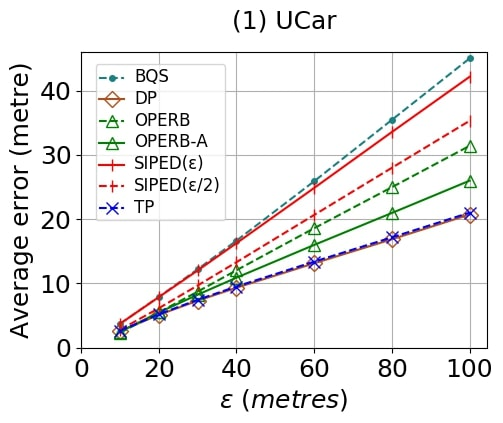
\includegraphics[scale=0.250]{Figures/Exp-PED-error-epsilon-service.jpg}	\hspace{0.5ex}
	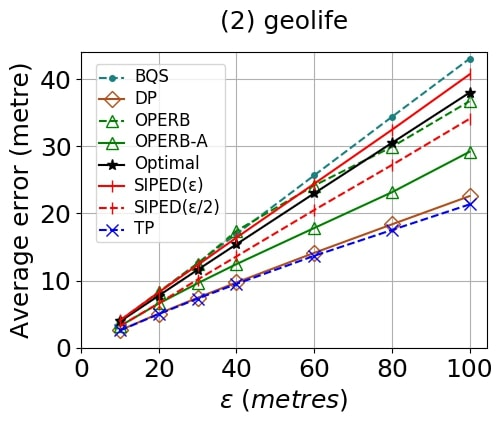
\includegraphics[scale=0.250]{Figures/Exp-PED-error-epsilon-geolife.jpg}	\hspace{0.5ex}
	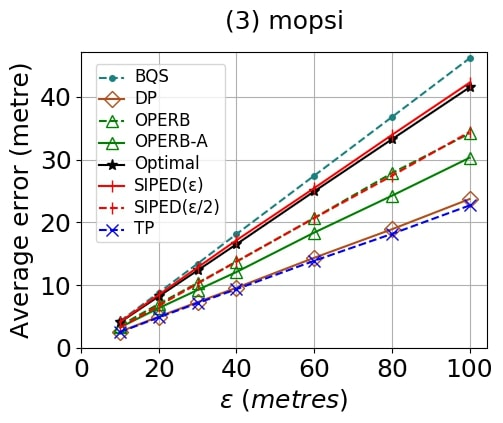
\includegraphics[scale=0.250]{Figures/Exp-PED-error-epsilon-mopsi.jpg}	
	\vspace{-2ex}
	\caption{\small Evaluation of average errors (\ped) on full datasets: varying the error bound $\epsilon$.}
	\label{fig:ae-ped-epsilon}
	\vspace{-2ex}
\end{figure*}

\begin{figure*}[tb!]
	\centering
	%\includegraphics[scale=0.250]{Figures/Exp-SED-error-epsilon-taxi.jpg} \hspace{0.5ex}
	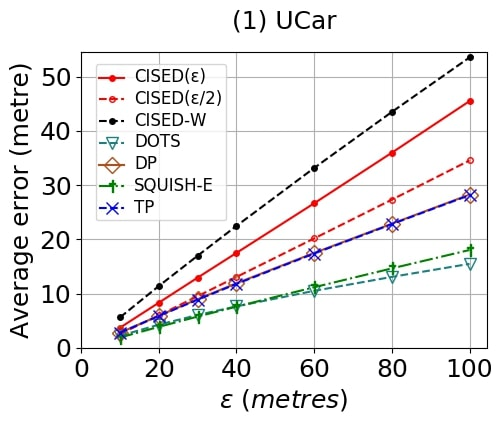
\includegraphics[scale=0.250]{Figures/Exp-SED-error-epsilon-service.jpg}	\hspace{0.5ex}
	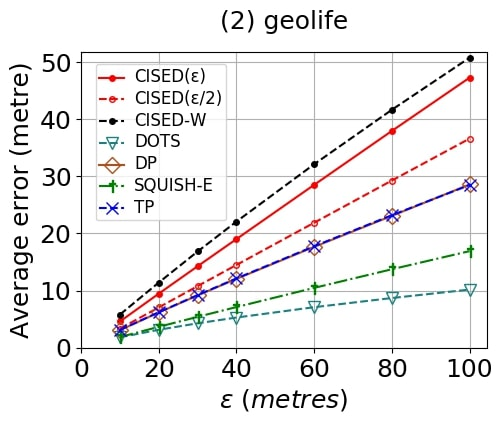
\includegraphics[scale=0.250]{Figures/Exp-SED-error-epsilon-geolife.jpg}	\hspace{0.5ex}
	\includegraphics[scale=0.250]{Figures/Exp-SED-error-epsilon-mopsi.jpg}		
	\vspace{-2ex}
	\caption{\small Evaluation of average errors (\sed) on full datasets: varying the error bound $\epsilon$.}
	\label{fig:ae-sed-epsilon}
	\vspace{-2ex}
\end{figure*}

\begin{figure*}[tb!]
	\centering
	%\includegraphics[scale=0.250]{Figures/Exp-DAD-error-epsilon-taxi.jpg} \hspace{0.5ex}
	\includegraphics[scale=0.348]{Figures/Exp-DAD-error-epsilon-service.jpg}	\hspace{0.5ex}
	\includegraphics[scale=0.348]{Figures/Exp-DAD-error-epsilon-geolife.jpg}	\hspace{0.5ex}
	\includegraphics[scale=0.3480]{Figures/Exp-DAD-error-epsilon-mopsi.jpg}	
	\vspace{-2ex}
	\caption{\small Evaluation of average errors (\dad) on full datasets: varying the error bound $\epsilon$.}
	\label{fig:ae-dad-epsilon}
	\vspace{-2ex}
\end{figure*}




\sstab (1) {Datasets \textcolor{blue}{and data sizes} are insensitive to the errors of \lsa algorithms.}

\sstab (2) When using \ped, the average errors from the smallest
to the largest are batch algorithms \tpa and \dpa, one-pass
algorithm \myblue{\operb-A}, one-pass
algorithms \siped($\frac{\epsilon}{2}$) and \operb, the optimal algorithm \opt and one-pass algorithm \siped(${\epsilon}$), and online algorithm \bqsa.
%
For full datasets, algorithms \tpa and \dpa are comparable, and they are on average ($58.69\%$, $61.34\%$,
$57.57\%$) and ($57.61\%$, $62.66\%$, $60.23\%$) of \opt on datasets \dSets, respectively.
Algorithms \siped($\frac{\epsilon}{2}$) and \operb are comparable, and they are on average
($80.96\%$, $79.12\%$, $79.33\%$) and ($70.60\%$, $76.64\%$, $78.71\%$) of \opt on datasets \dSets, respectively.
%
Algorithms \myblue{\operb-A}, \siped(${\epsilon}$) and \bqsa are on average \myblue{$(71.17\%, 80.10\%, 69.82\%)$}, ($100.05\%$, $101.01\%$, $102.69\%$) and ($104.67\%$, $108.91\%$, $106.92\%$) of \opt on datasets \dSets, respectively.
For example, the average errors of algorithms
(\opt, \tpa, \dpa, \bqsa, \siped(${\epsilon}$), \siped($\frac{\epsilon}{2}$), \operb, \myblue{\operb-A} ) in the full \mopsi are ($16.08$, $9.19$, $9.68$, $17.4$, $12.96$, $16.83$, $12.77$, \myblue{$12.45$}) metres when $\epsilon$ = $40m$.

\eat{
In Figure~\ref{fig:ae-ped-size}, algorithms \tpa and \dpa are comparable, and they are on average
{($105.94\%$, $53.16\%$, $66.84\%$, $61.50\%$), ($111.96\%$, $52.04\%$, $78.65\%$, $60.57\%$)} of \opt on datasets \dSets, respectively.
Algorithms \siped($\frac{\epsilon}{2}$) and \operb are on average {($85.30\%$, $73.55\%$, $82.01\%$,
  $85.23\%$), ($97.69\%$, $67.20\%$, $82.58\%$, $81.88\%$)}
of \opt on datasets \dSets, respectively.
Algorithm \bqsa is  on average  {($108.51\%$, $102.06\%$, $104.63\%$, $113.80\%$)}
of \opt on datasets \dSets, respectively.
}



\begin{figure*}[tb!]
	\centering
	%\includegraphics[scale=0.250]{Figures/Exp-PED-error-size-taxi.jpg}\hspace{0.5ex}
	\includegraphics[scale=0.250]{Figures/Exp-PED-error-size-service.jpg} 	\hspace{0.5ex}
	\includegraphics[scale=0.250]{Figures/Exp-PED-error-size-geolife.jpg}	\hspace{0.5ex}
	\includegraphics[scale=0.250]{Figures/Exp-PED-error-size-mopsi.jpg}		
	\vspace{-2ex}
	\caption{\small Evaluation of average errors (\ped) on small datasets: varying the size of
		trajectories.}
	\label{fig:ae-ped-size}
	\vspace{-2ex}
\end{figure*}

\begin{figure*}[tb!]
	\centering
	%\includegraphics[scale=0.250]{Figures/Exp-SED-error-size-taxi.jpg}\hspace{0.5ex}
	\includegraphics[scale=0.250]{Figures/Exp-SED-error-size-service.jpg} 	\hspace{0.5ex}
	\includegraphics[scale=0.250]{Figures/Exp-SED-error-size-geolife.jpg}	\hspace{0.5ex}
	\includegraphics[scale=0.348]{Figures/Exp-SED-error-size-mopsi.jpg}		
	\vspace{-2ex}
	\caption{\small Evaluation of average errors (\sed) on small datasets: varying the size of
		trajectories.}
	\label{fig:ae-sed-size}
	\vspace{-2ex}
\end{figure*}


\begin{figure*}[tb!]
	\centering
	%\includegraphics[scale=0.50]{Figures/Exp-DAD-error-size-taxi.jpg} \hspace{0.5ex}
	\includegraphics[scale=0.52]{Figures/Exp-DAD-error-size-service.jpg}	\hspace{0.5ex}
	\includegraphics[scale=0.52]{Figures/Exp-DAD-error-size-geolife.jpg}	\hspace{0.5ex}
	\includegraphics[scale=0.52]{Figures/Exp-DAD-error-size-mopsi.jpg}	
	\vspace{-2ex}
	\caption{\small Evaluation of average errors (\dad) on small datasets: varying the size of trajectories.}
	\label{fig:ae-dad-size}
	\vspace{-2ex}
\end{figure*}



\sstab (3) When using \sed, the average errors from the smallest
to the largest are online algorithm {\dagots}, online algorithm \squishe, batch algorithms \tpa and \dpa,
one-pass algorithm \cised($\frac{\epsilon}{2}$),  the \opt algorithm and one-pass algorithm \cised(${\epsilon}$), and one-pass algorithm \myblue{\cised-W}.
%
Algorithms \tpa and \dpa are comparable, and they are on average
{($60.36\%$, $66.11\%$, $62.43\%$) and ($62.54\%$, $67.04\%$, $68.64\%$)} of \opt on datasets \dSets, respectively.
Algorithms \myblue{\cised-W}, \cised(${\epsilon}$), \cised($\frac{\epsilon}{2}$), \squishe and {\dagots} are on average {\myblue{$(115.24\%, 120.34\%, 123.40\%)$}, ($97.32\%$, $106.74\%$, $108.16\%$), ($75.29\%$, $76.03\%$, $81.44\%$), ($40.61\%$, $38.15\%$, $34.22\%$) and \myblue{$(39.12\%, 28.80\%, 23.90\%)$} of \opt on datasets \dSets, respectively.
%
For example, the average errors of algorithms
(\opt, \tpa, \dpa, \squishe, \myblue{\dagots}, \cised(${\epsilon}$), \cised($\frac{\epsilon}{2}$),  \myblue{\cised-W}) in full \mopsi are ($19.39$, $12.17$, $12.20$,  $6.76$, \myblue{$4.67$}, $20.68$, $14.71$,  \myblue{$24.12$}) metres, respectively, when $\epsilon$ = $40m$.
%


\sstab {(4) When using \dad, the average errors from the smallest
to the largest are one-pass algorithm \intersec, batch algorithms \dpa and \tpa, one-pass algorithm \interval and online algorithm \opwa, and the optimal algorithm \opt.
\eat{%%%%%%%%%%%%%
For example, in Figure~\ref{fig:ae-dad-ped-epsilon}, in \mopsi, the average errors of algorithms
(\tpa, \dpa, \interval) in terms of \ped are ($65.6$, $75.4$, $68.1$) meters, respectively, when $\epsilon$ = $45$ degrees.
It is also worth pointing out that the max errors of algorithms
(\tpa, \dpa, \interval) using \dad may be very large in terms of \ped, \eg they are ($68247.9$, $66794.4$, $68247.9$) meters, respectively, when $\epsilon$ = $45$ degrees.}
}%%%%%%%%%%%%%
Algorithms \tpa, \opwa and \interval are comparable, and they are on average
{($91.35\%$, $61.45\%$, $73.71\%$), ($91.95\%$, $61.37\%$, $76.17\%$) and ($90.36\%$, $68.23\%$, $163.47\%$)} of \opt on datasets \dSets, respectively.
Algorithms \intersec and \dpa are on average ($62.03\%$, $76.54\%$, $110.69\%$) and ($82.45\%$, $96.52\%$, $137.95\%$) of \opt on datasets \dSets, respectively.




We then present analyses from the views of \lsa algorithms and distance metrics.


\stitle{Analyses of \lsa algorithms}. The average errors of these algorithms  are generally on the contrary of compression ratios. The optimal algorithm is usually  the worst algorithm in terms of average errors, followed by one-pass algorithms and then batch algorithms.
Online algorithms have varied average errors, ranging from the best to the worst.
(1) For batch algorithms, both bottom-up algorithm (\tpa) and top-down algorithm (\dpa) have similar average errors, and they are pretty good compared with other algorithms.
%
(2) Online algorithms \bqsa and \opwa often have the largest average errors in all sub-optimal algorithms, while \myblue{\dagots}~and \squishe have the smallest. This is also on the contrary of their compression ratios.
%
(3) For one-pass algorithms, the full $\epsilon$ sector/cone/range combining with a position/direction constraint always have larger average errors than the half $\epsilon$ sector/cone/range.
%
Local distance checking approaches try to include more points into a line segment, this greedy strategy is likely leading to larger average errors, considerable larger than batch algorithms that have the similar compression ratios as one-pass and online algorithms.


\stitle{Analyses of distance metrics}.
For the same error bound $\epsilon$, the average errors of algorithms using \sed are a bit larger than using \ped. {As we know that \ped error is originally caused by the direction changes of a moving object while \sed error is caused by the changes of both the direction and the speed of a moving object, the above phenomenon probably reveals that the changes of speeds are more frequent than the changes of directions for moving objects.}
%
And in practice (\eg $\epsilon = 60$ meters and $\epsilon = 45$ degrees), the average errors of algorithms using \dad, when translated to position errors like \ped, are likely $10$ times larger than algorithms directly using \ped and \sed. This is obvious as a small direction deviation with a long trip may lead to a large position error.




\eat{
\sstab (1) When increasing $\epsilon$, the average errors increase linearly.

\sstab (2) Datasets have few impacts on the average errors.

\sstab (1) Trajectory sizes have few impacts on average errors.

\sstab (2) The average errors in this test are consistent with test Exp-2.1.
}






%%%%%%%%%%%%%%%%%%%%%%%%%%%%%%%%%%%%%%%%%%%%%%%%%%%%%%%%%%%%%%%%%%%%%%%%%%%%%%
%\vspace{-1ex}
\subsubsection{Evaluation and Analyses of Efficiency}
%%%%%%%%%%%%%%%%%%%%%%%%%%%%%%%%%%%%%%%%%%%%%%%%%%%%%%%%%%%%%%%%%%%%%%%%%%%%%%

In this set of tests, we compare the efficiency of these algorithms.
The results are reported in Figures~\ref{fig:time-epsilon-ped},~\ref{fig:time-epsilon-sed},~\ref{fig:time-epsilon-dad},~\ref{fig:time-size-ped},~\ref{fig:time-size-sed} and~\ref{fig:time-size-dad}.
Note that even on the small datasets, \emph{the running time of algorithm \opt  is thousands of times slower than one-pass algorithms}. As it is not clear to show all these algorithms in a single figure, only the results of sub-optimal algorithms are shown in these figures.
We first report our findings.



\sstab (1) {Datasets do not have obvious impacts on the running time of \lsa algorithms except \dagots. }

	
\sstab (2) When using \ped, in most cases, the running time from the smallest to the largest is one-pass algorithms \siped, \operb and \myblue{\operb-A}, batch algorithms \tpa and \dpa, and online algorithm \bqsa.
Algorithms \siped($\frac{\epsilon}{2}$), {\operb} and \myblue{\operb-A} are comparable, algorithm \siped(${\epsilon}$) is $(0.92, 0.92, 0.91)$ times of \siped($\frac{\epsilon}{2}$), and algorithms \tpa, \dpa and \bqsa are on average
($26.79$, $28.25$, $29.87$), ($16.32$, $15.40$, $11.02$) and ($37.73$, $62.23$, $61.29$)
times slower than one-pass algorithm \siped($\frac{\epsilon}{2}$) on datasets \dSets, respectively.
For example, in \mopsi, the running time of algorithms
(\tpa, \dpa, \bqsa, \siped(${\epsilon}$), \siped($\frac{\epsilon}{2}$), \operb, \myblue{\operb-A} ) is ($232.9$, $124.2$, $469.4$, $6.89$, $7.6$, $8.6$, {$9.4\%$}) seconds when $\epsilon$ = $40m$.



\begin{figure*}[tb!]
	\centering
	%\includegraphics[scale=0.250]{Figures/Exp-PED-time-epsilon-taxi.jpg}	\hspace{0.5ex}
	\includegraphics[scale=0.250]{Figures/Exp-PED-time-epsilon-service.jpg}	\hspace{0.5ex}
	\includegraphics[scale=0.250]{Figures/Exp-PED-time-epsilon-geolife.jpg}	\hspace{0.5ex}
	\includegraphics[scale=0.250]{Figures/Exp-PED-time-epsilon-mopsi.jpg}	
	\vspace{-2ex}
	\caption{\small Evaluation of running time (\ped) on full datasets: varying the error bound $\epsilon$.}\label{fig:time-epsilon-ped}
	\vspace{-2ex}
\end{figure*}

\begin{figure*}[tb!]
	\centering
	%\includegraphics[scale=0.250]{Figures/Exp-SED-time-epsilon-taxi.jpg}	\hspace{0.5ex}
	\includegraphics[scale=0.250]{Figures/Exp-SED-time-epsilon-service.jpg}	\hspace{0.5ex}
	\includegraphics[scale=0.250]{Figures/Exp-SED-time-epsilon-geolife.jpg}	\hspace{0.5ex}
	\includegraphics[scale=0.250]{Figures/Exp-SED-time-epsilon-mopsi.jpg}	
	\vspace{-2ex}
	\caption{\small Evaluation of running time (\sed) on full datasets: varying the error bound $\epsilon$.}\label{fig:time-epsilon-sed}
	\vspace{-2ex}
\end{figure*}

\begin{figure*}[tb!]
	\centering
	%\includegraphics[scale=0.250]{Figures/Exp-DAD-time-epsilon-taxi.jpg}\hspace{0.5ex}
	\includegraphics[scale=0.250]{Figures/Exp-DAD-time-epsilon-service.jpg} 	\hspace{0.5ex}
	\includegraphics[scale=0.250]{Figures/Exp-DAD-time-epsilon-geolife.jpg}	\hspace{0.5ex}
	\includegraphics[scale=0.250]{Figures/Exp-DAD-time-epsilon-mopsi.jpg}		
	\vspace{-2ex}
	\caption{\small Evaluation of running time (\dad) on full datasets: varying the error bound $\epsilon$.}\label{fig:time-epsilon-dad}
	\vspace{-2ex}
\end{figure*}



\sstab (3) When using \sed, the running time of algorithms except \dagots~from the smallest to the largest is one-pass algorithms \cised and \myblue{\cised-W}, online algorithm \squishe, and batch algorithms \tpa and \dpa, while \dagots~has varied running time. In full datasets, \dagots~runs faster than, comparable with and slower than \dpa in datasets \ucar, \geolife and \mopsi, respectively, while in small datasets, it often runs fast than \dpa. 
Algorithm \cised(${\epsilon}$) is $(1.17, 1.17, 0.91)$ times of \cised($\frac{\epsilon}{2}$), and algorithms \tpa, \dpa and \squishe are on average
 ($13.33$, $15.81$, $13.09$), ($12.93$, $10.64$, $8.79$) and
($2.75$, $2.78$, $2.57$) times slower than \cised($\frac{\epsilon}{2}$) on datasets \dSets, respectively.
%
For example, in \mopsi, the running time of algorithms
(\tpa, \dpa, {\dagots}, \squishe, \cised($\epsilon$), \cised($\frac{\epsilon}{2}$), \myblue{\cised-W}) is ($156.6$, $104.8$, \myblue{$361.1$}, $27.2$, $11.6$, $9.7$, \myblue{$9.7$}) seconds when $\epsilon$ = $40m$.

\sstab {(4) When using \dad,} \textcolor{blue}{one-pass algorithms \intersec and \interval run prominently faster than batch algorithms \tpa and \dpa and online algorithm \opwa.}
%
%Algorithm \interval is a bit slower than \intersec, and algorithms \tpa and \dpa are on average
%($6.66$, $13.55$, $12.73$, $12.73$) and ($11.67$, $14.24$, $16.51$, $17.59$)
%times slower than \interval on datasets \dSets, respectively.
%
Algorithm \interval is $(1.80, 1.84, 1.81)$ times slower than \intersec, and algorithms \tpa, \dpa and \opwa are on average
($24.63$, $23.53$, $23.23$), ($25.49$, $30.11$, $31.72$) and ($39.29$, $147.85$, $80.09$)
times slower than \intersec on datasets \dSets, respectively.
%
For example, the running time of algorithms
(\tpa, \dpa, \opwa, \interval, \intersec) is ($105.57$, $152.53$, $240.40$, $8.57$, $4.69$) seconds in \mopsi when
$\epsilon=45$ degrees, respectively.



\begin{figure*}[tb!]
	\centering
	%\includegraphics[scale=0.250]{Figures/Exp-PED-time-size-taxi.jpg}\hspace{0.5ex}
	\includegraphics[scale=0.250]{Figures/Exp-PED-time-size-service.jpg}	\hspace{0.5ex}
	\includegraphics[scale=0.250]{Figures/Exp-PED-time-size-geolife.jpg}	\hspace{0.5ex}
	\includegraphics[scale=0.250]{Figures/Exp-PED-time-size-mopsi.jpg}	
	\vspace{-2ex}
	\caption{\small Evaluation of running time (\ped) on small datasets: varying the size of trajectories.}\label{fig:time-size-ped}
	\vspace{-2ex}
\end{figure*}

\begin{figure*}[tb!]
	\centering
	%\includegraphics[scale=0.250]{Figures/Exp-SED-time-size-taxi.jpg}\hspace{0.5ex}
	\includegraphics[scale=0.250]{Figures/Exp-SED-time-size-service.jpg}	\hspace{0.5ex}
	\includegraphics[scale=0.250]{Figures/Exp-SED-time-size-geolife.jpg}	\hspace{0.5ex}
	\includegraphics[scale=0.348]{Figures/Exp-SED-time-size-mopsi.jpg}	
	\vspace{-2ex}
	\caption{\small Evaluation of running time (\sed) on small datasets: varying the size of trajectories.}\label{fig:time-size-sed}
	\vspace{-2ex}
\end{figure*}

\begin{figure*}[tb!]
	\centering
	%\includegraphics[scale=0.50]{Figures/Exp-DAD-time-size-taxi.jpg}\hspace{0.5ex}
	\includegraphics[scale=0.52]{Figures/Exp-DAD-time-size-service.jpg} 	\hspace{0.5ex}
	\includegraphics[scale=0.52]{Figures/Exp-DAD-time-size-geolife.jpg}	\hspace{0.5ex}
	\includegraphics[scale=0.52]{Figures/Exp-DAD-time-size-mopsi.jpg}		
	\vspace{-2ex}
	\caption{\small Evaluation of running time (\dad) on small datasets: varying the size of trajectories.}\label{fig:time-size-dad}
	\vspace{-2ex}
\end{figure*}


%\sstab (2) When using \ped, the running time from the smallest to the largest are one-pass algorithms \siped and \operb, and batch and online algorithms \tpa, \dpa and \bqsa. Algorithms \siped and \operb are comparable. Algorithms \tpa, \dpa and \bqsa are comparable, and they are on average \textcolor{red}{($3.8$--$5.3$, $3.5$--$4.8$, $4.6$--$7.2$, $6.2$--$8.4$)} times slower than the one-pass algorithms \siped and \operb on datasets \dSets, respectively.

%\sstab (3) When using \sed, the running time from the smallest to the largest are one-pass algorithm \cised, online algorithm \squishe, and batch algorithms \tpa and \dpa.  Algorithms \squishe, \tpa and \dpa are on average \textcolor{red}{($9.6$--$17.6$, $8.8$--$15.4$, $8.4$--$16.3$, $9.0$--$14.4$)}, \textcolor{red}{($9.6$--$17.6$, $8.8$--$15.4$, $8.4$--$16.3$, $9.0$--$14.4$)} and \textcolor{red}{($9.6$--$17.6$, $8.8$--$15.4$, $8.4$--$16.3$, $9.0$--$14.4$)} times slower than \cised on datasets \dSets, respectively.

%\sstab (4) Batch algorithms \dpa and \tpa using \sed run a bit faster than using \ped, while the one-pass algorithm \cised run \textcolor{red}{$2.0$--$3.0$} times slower than \siped and \operb.


We then present analyses from the views of \lsa algorithms and distance metrics.





\stitle{Analyses of \lsa algorithms.}
The running time from the fastest to the slowest is one-pass algorithms, online and batch algorithms, and optimal algorithms.

For batch algorithms, the running time of \dpa and \tpa decreases or increases with the increase of error bound $\epsilon$, respectively, due to the top-down and bottom-up approaches that they apply. When using \ped or \sed, top-down algorithm usually runs faster than bottom-up algorithm when the error bound $\epsilon$~is large (\eg in \geolife, $\epsilon >10$ metres when using \ped and $\epsilon >30$ metres when using \sed), which means that top-down (bottom-up) algorithm needs to split (merge) the original trajectory fewer (more) times in these cases, vice versa. When using \dad,  top-down algorithms are normally a bit slower than bottom-up algorithms (recall that top-down algorithms have poorer compression ratios compared with bottom-up algorithms, which means that it needs more time to split the raw trajectory into more sub trajectories).
In addition to error bounds, sampling rates also have impacts on the efficiency of batch algorithms. A dataset with high sampling rate likely needs more merging processes than splitting processes, thus, top-down algorithms run faster than bottom-up algorithms in high sampling datasets when using \ped or \sed.

For online algorithms, \squishe is faster than \bqsa and \opwa at a cost of poorer compression ratios, and it is still a few times slower than one-pass algorithms. \bqsa and \opwa both have poor efficiency as they finally need batch approaches to simplify buffered data, and batch approaches running in a buffer are still time consuming. \textcolor{blue}{\dagots~runs slowly in full datasets, partially because it is implemented in Java, in which the frequent copies of memory waste a lot of time (its C/C++ version is faster than \squishe as reported in \cite{Zhang:Evaluation}) and become its bottleneck of efficiency.}

For one-pass algorithms, \operb, \siped, \cised and \interval show a linear running time that is consistent with their time complexity analyses. They are not very sensitive to error bound $\epsilon$, and also scale well with the increase of trajectory size on all datasets as a data point is processed only one time during the whole process.
Algorithms \siped, \operb and \interval have similar running time, and algorithm \cised runs a bit slower than them, partially because finding the common intersection of spatial-temporal cones is a heavier work than sectors or ranges. 
\textcolor{blue}{Besides, weak simplification algorithms have similar running time as their corresponding strong algorithms.}



\stitle{Analyses of distance metrics.}
The computation time of \dad is faster than \ped and \sed, and the computation time of \ped and \sed are 2.3 and 1.7 times of \dad, respectively.
{It is also worth pointing out that algorithms \dpa using \ped, \sed and \dad have similar running time in all datasets, though the computation of \ped is much heavier than \sed and \dad. The reason is that \dpa using \ped has the best compression ratios which instead leads to the least splitting processes in the top-down manner. Combining these two factors, \ie the computing of distance/direction deviation and the processing of trajectory splitting, finally, algorithm \dpa using \ped has similar running time as \dpa using \dad or \sed.}

%%%%%%%%%%%%%%%%%%%%%%%%%%%%%%%%%%%%%%%%%%%%%%%%%%%%%%%%%%%%%%%%%%%%%%%%%%%%%%
\subsubsection{{Evaluation and Analyses of Data Aging}}
%%%%%%%%%%%%%%%%%%%%%%%%%%%%%%%%%%%%%%%%%%%%%%%%%%%%%%%%%%%%%%%%%%%%%%%%%%%%%%
\label{sec:exp-data-aging}
In this set of tests, we compare the errors and compression ratios of algorithms in data aging. We set $\epsilon_1=40m$ (or $\epsilon_1=30^o$) in the first run and $\epsilon_2=60m$ (or $\epsilon_2=50^o$) in the second run. Besides, we also run these algorithms on the raw trajectories, setting $\epsilon_3=\epsilon_1 + \epsilon_2=100m$ (or $\epsilon_3=80^o$). The max errors are reported in \mytable{tab:aging-me}, and the compression ratios are reported in \mytable{tab:aging-cr} and \mytable{tab:cr}, respectively.

\ni (1) Algorithms \dpa using \ped and \sed both have max errors less than $\epsilon_2 = 60m$, confirming that they are aging friendly and their max errors are consistent with Theorem ~\ref{theo-aging-error-dp}; while algorithm \dpa using \dad and other algorithms have max error larger than $\epsilon_2 = 60m$ or $\epsilon_2 = 50^o$, confirming that they are not aging friendly and their max errors are consistent with Theorems ~\ref{theo-aging-dp-dad}, \ref{theo-aging-tp} and \ref{theo-aging-online}.

\ni (2) Algorithm \dpa using \dad and other algorithms have max error less than $\epsilon_1 + \epsilon_2 = 100m$ or $\epsilon_1 + \epsilon_2 = 80^o$, which is consistent with Theorem ~\ref{theo-aging-distance}.

\ni (3) \mytable{tab:aging-cr} and \mytable{tab:cr} tell that, if algorithms compress data using $\epsilon_1$ and $\epsilon_2$ in turn, then they have a bit poorer compression ratios than directly using $\epsilon_3=\epsilon_1 + \epsilon_2$.
Note that the causes of this phenomenon are varied. For algorithm \dpa using \ped or \sed, it is caused by the shorten of the final error bound, which is $max\{\epsilon_1, \epsilon_2\}$, less than $\epsilon_3=\epsilon_1 + \epsilon_2$; while for the other algorithms, they lose some compression ratios because of data aging.

%In the contrast, algorithms \dpa using \ped and \sed do not loss that. Hence, given the same final error bound (\eg $100m$) of data aging, algorithm \dpa using \ped (or \sed) shows a bit advantages in terms of compression ratios.



\stitle{Analyses of \lsa algorithms.} \dpa is the only algorithm that is aging friendly \wrt ~\ped and \sed, \myblue{and all algorithms have bounded errors}. Indeed, {aging friendly} is a result of the {specific nature} of algorithm \dpa, \ie batch and top-down, that always splits a trajectory into two sub trajectories by the same splitting point when it uses any \ped or \sed larger than the error bound.

\stitle{Analyses of \lsa distance metrics.} \dad is not aging friendly \wrt to any algorithm. It is different with \ped and \sed in that, the \dad of a point is closely related to its neighbor point while \ped and \sed are not, thus, once its neighbor point is removed, its \dad is also changed. This character makes it not aging friendly \wrt the \dpa algorithm.


\begin{table}
	%\renewcommand{\arraystretch}{1.2}
	\caption{\small The max errors of algorithms in data aging that set $\epsilon_1=40m$ (or $\epsilon_1=30^o$ when using \dad) in the first run and $\epsilon_2=60m$ (or $\epsilon_2=50^o$ when using \dad) in the second run.}
	\centering
	\scriptsize
	\vspace{-1ex}
	\begin{tabular}{|l|c|c|c|l|c|c|c|l|c|c|c|}
		\hline
		\bf{Alg. (PED)}  &\ucar &\geolife &\mopsi & \bf{Alg. (SED)}  &\ucar &\geolife &\mopsi &\bf{Alg. (DAD)}  &\ucar &\geolife &\mopsi \\
		\hline
		{\dpa} &	$59.99$ & $59.99 $ &	$59.99$	&\dpa &$59.99$ &$59.99$ & $59.99$ & \dpa	& $79.90$	& $79.93$	& $78.96 $ \\
		\hline
		{\tpa} &	$99.56$ & $96.95$ &	$93.00$	&\tpa 	& $97.55$& $96.70$ &$90.53$ & \tpa	& $79.94$	& $79.93$	& $79.64$ \\
		\hline
		{\bqsa} &	$96.20 $ & $93.58  $ &	$96.79 $	&\squishe &$92.60$ &$90.89$ & $84.38$ & \opwa	& $79.96$	& $79.96$	& $79.74$ \\
		\hline
		{\siped($\epsilon$)} &	$97.34   $ & $95.21  $ &	$98.86   $	&\cised($\epsilon$) & $97.75$ &$97.51$ &$96.65$ & \interval	& $79.96$	& $79.93$	& $79.74$ \\
		\hline
		{\siped($\frac{\epsilon}{2}$)} &	$99.18  $ & $94.57  $ &	$97.91  $ &\cised($\frac{\epsilon}{2}$) &$ 97.40 $ & $97.51$ & $98.83$& \intersec	& $70.26 $	& $77.78$	& $72.87$ \\
		\hline
		{\operb} &	${98.26} $ & ${96.53} $ & ${98.08} $	& \textcolor{blue}{\dagots} &98.47 &95.92 &96.7 & / &- &- &- \\
		\hline
		\textcolor{blue}{\operb-A} &	${99.99} $ & ${99.99} $ & ${99.99} $	& \textcolor{blue}{\cised-W} &99.21 &99.34 &98.81 & / &- &- &- \\
		\hline
	\end{tabular}
	\label{tab:aging-me}

	\vspace{-2ex}
\end{table}


   	 	
\begin{table}
	%\renewcommand{\arraystretch}{1.2}
	\caption{\small The final compression ratios of algorithms in data aging that set $\epsilon_1=40m$ (or $\epsilon_1=30^o$ when using \dad) in the first run and $\epsilon_2=60m$ (or $\epsilon_2=50^o$ when using \dad) in the second run.}
	\centering
	\scriptsize
	\vspace{-1ex}
	\begin{tabular}{|l|c|c|c|l|c|c|c|l|c|c|c|}
		\hline
		\bf{Alg. (PED)}  &\ucar &\geolife &\mopsi & \bf{Alg. (SED)}  &\ucar &\geolife &\mopsi &\bf{Alg. (DAD)}  &\ucar &\geolife &\mopsi \\
		\hline  		
		{\dpa} &	$4.67$ & $1.94 $ &	$1.68$	&\dpa &$10.03$ &$3.83$ & $2.78 $ & \dpa	& $12.75$	& $22.20$	& $20.34 $ \\
		\hline
		{\tpa} &	$4.66$ & $	2.07 $ &	$1.74 $	&\tpa 	& $10.09$& $3.78$ &$2.76$ & \tpa	& $3.80$	& $13.28$	& $11.30$ \\
		\hline
		{\bqsa} &	$4.13$ & $1.67 $ &	$ 1.43 $	&\squishe &$11.38$ &$4.55$ & $3.47$ & \opwa	& $4.09$	& $13.88$	& $11.92$ \\
		\hline
		{\siped($\epsilon$)} &	$4.15 $ & $1.69 $ &	$1.42$	&\cised($\epsilon$) & $9.12$ &$3.28$ &$2.45 $ & \interval	& $3.81$	& $13.37$	& $11.47 $ \\
		\hline
		{\siped($\frac{\epsilon}{2}$)} &	$4.65 $ & $1.94$ &	$1.68$ &\cised($\frac{\epsilon}{2}$) &$10.66 $ & $3.94$ & $2.99 $& \intersec	& $5.37$	& $17.11$	& $15.05 $ \\
		\hline
		{\operb} &	$5.03$ & $2.03 $ &	$ 1.97 $	& \textcolor{blue}{\dagots} &11.81 &3.89 &2.55 & / &- &- & - \\
		\hline
		\textcolor{blue}{\operb-A} &	${5.53} $ & ${1.90} $ & ${1.93} $	& \textcolor{blue}{\cised-W} &8.94 &3.76 &2.34 & / &- &- &- \\
		\hline
	\end{tabular}
	\label{tab:aging-cr}	
	\vspace{-2ex}
\end{table}

 	 	
   	 	
\begin{table}
	%\renewcommand{\arraystretch}{1.2}
	\caption{\small The compression ratios of algorithms running on the raw trajectories that set $\epsilon_3=\epsilon_1+\epsilon_2=100m$ (or $\epsilon_3=80^o$ when using \dad).}
	\centering
	\scriptsize
	\vspace{-1ex}
	\begin{tabular}{|l|c|c|c|l|c|c|c|l|c|c|c|}
		\hline
		\bf{Alg. (PED)}  &\ucar &\geolife &\mopsi & \bf{Alg. (SED)}  &\ucar &\geolife &\mopsi &\bf{Alg. (DAD)}  &\ucar &\geolife &\mopsi \\
		\hline
		{\dpa} &	$3.64$ & $ 1.17$ &	$1.39$	&\dpa &$7.44$ & $2.69$ &$1.91$  & \dpa	& $8.25$	& $15.17$	& $17.04$ \\
		\hline
		{\tpa} &	$3.70 $ & $1.22$ &	$1.50 $	&\tpa 	& $7.56 $& $2.70$ & $1.73 $ & \tpa	& $2.47 $	& $ 	7.51 $	& $ 	9.42  $ \\
		\hline
		{\bqsa} &	$3.23$ & $1.71$ &	$1.39 $	&\squishe &$10.36 $ & $4.10  $ & $2.82$ & \opwa	& $3.23$	& $8.66$	& $10.75$ \\
		\hline
		{\siped($\epsilon$)} &	$3.25$ & $ 1.04$ &	$1.28 $	&\cised($\epsilon$) & $6.68 $ &$ 2.35$ &$ 1.49	$ & \interval	& $2.79 $	& $8.01$	& $9.95 $ \\
		\hline
		{\siped($\frac{\epsilon}{2}$)} &	$3.81 $ & $1.29 $ &	$1.55 $ &\cised($\frac{\epsilon}{2}$) &$8.02  $ & $2.90$ & $1.87$& \intersec	& $4.32 $	& $11.75$	& $13.61 $ \\
		\hline
		{\operb} &	$4.08 $ & $1.43 $ & $1.56 $	& \textcolor{blue}{\dagots} &10.91 &4.33 &3.43 & /&- &- &- \\
		\hline
		\textcolor{blue}{\operb-A} &	${4.06} $ & ${1.31} $ & ${1.20} $	& \textcolor{blue}{\cised-W} &6.92 &2.98 &1.77 & / &- &- &- \\
		\hline
	\end{tabular}
	\label{tab:cr}	
	\vspace{-2ex}
\end{table}
 	 	
 	 	
 	 	


%%%%%%%%%%%%%%%%%%%%%%%%%%%%%%%%%%%%%%%%%%%%%%%%%%%%%%%%%%%%%%%%%%%%%%%%%%%%%%
\subsubsection{{Evaluation and Analyses of Queries Friendliness}}
\label{sec-exp-query}
%%%%%%%%%%%%%%%%%%%%%%%%%%%%%%%%%%%%%%%%%%%%%%%%%%%%%%%%%%%%%%%%%%%%%%%%%%%%%%
We finally evaluate those compressed trajectories from the viewpoint of trajectory application, \ie spatio-temporal query. The well-known spatio-temporal queries are \emph{where\_at, when\_at, range, nearest\_neighbor} and \emph{spatial\_join} \cite{Cao:Spatio,Trajcevski:Uncertainty}. Among them, \emph{where\_at} query, \ie ``\emph{the position $P$ of a moving object at time $t$}" \cite{Cao:Spatio}, is the foundation of \emph{range} and \emph{nearest\_neighbor} queries, \textcolor{blue}{and \emph{when\_at} query, \ie ``\emph{the time $t$ at which a moving object on a trajectory is expected to be at position $P$}" \cite{Cao:Spatio}, is also a critical building block for many applications.}
{Hence, we choose them to evaluate compressed trajectories simplified by \lsa algorithms using \ped, \sed and \dad.
As mentioned in \cite{Cao:Spatio,Trajcevski:Uncertainty}, the answer to \emph{where\_at} query is the expected position $P'$ of the moving object at time $t$. Indeed, it is the \emph{synchronized point} of $P$ when the query is performed on simplified trajectories.}

\stitle{\textcolor{blue}{Exp-1: \emph{where\_at} queries.}}
{We first compress these trajectories using \ped, \sed and \dad, respectively. }
{Then, for each point $P$ in an original trajectory $\dddot{\mathcal{T}}$, we perform a \emph{where\_at} query on each of its compressed trajectories taking time $P.t$ as input, and calculate the distance between the actual position $P$ and the expected position $P'$ to denote the error of queries.
}
%
{The max and average errors of the queries are reported in \mytable{tab:query-me} and Figures~\ref{fig:query-ped-epsilon}, \ref{fig:query-sed-epsilon}, \ref{fig:query-dad-epsilon}, \ref{fig:query-ped-size},\ref{fig:query-sed-size} and \ref{fig:query-dad-size}, respectively.}



\begin{table}
	%\renewcommand{\arraystretch}{1.2}
	\caption{\small The max errors of \textcolor{blue}{\emph{where\_at}} queries on compressed trajectories: fixed $\epsilon=40m$.}
	\centering
	\scriptsize
	\vspace{-1ex}
	\begin{tabular}{|l|c|c|c|l|c|c|c|}
		\hline
		\bf{Alg. (PED)}  &\ucar &\geolife &\mopsi & \bf{Alg. (DAD)}  &\ucar &\geolife &\mopsi \\
		\hline
		{\dpa} &	$3.48 \times 10^6$ & $1.83 \times 10^6$ &	$5.03 \times 10^6$	& \dpa	& $2.76 \times 10^6$	& $7.91 \times 10^5$	& $4.87 \times 10^5$ \\
		\hline
		{\tpa} &	$3.51 \times 10^6$ & $1.91 \times 10^6$ &	$5.03 \times 10^6$	& \tpa	& $2.76 \times 10^6$	& $7.91 \times 10^5$	& $5.01 \times 10^5$ \\
		\hline
		{\bqsa} &	$3.51 \times 10^6$ & $1.94 \times 10^6$ &	$1.40 \times 10^6$	& \opwa	& $2.76 \times 10^6$	& $7.91 \times 10^5$	& $5.01 \times 10^5$ \\
		\hline
		{\siped($\epsilon$)} &	$3.51 \times 10^6$ & $1.02 \times 10^6$ &	$1.39 \times 10^6$	& \interval	& $2.76 \times 10^6$	& $7.91 \times 10^5$	& $5.01 \times 10^5$ \\
		\hline
		{\siped($\epsilon/2$)} &	$3.50 \times 10^6$ & $1.02 \times 10^6$ &	$1.39 \times 10^6$	& \intersec	& $2.76 \times 10^6$	& $7.91 \times 10^5$	& $4.18 \times 10^5$ \\
		\hline
		{\operb} &	$3.50 \times 10^6$ & $1.56 \times 10^6$ &	$1.39 \times 10^6$	& / & -  & - & -  \\
		\hline
		\textcolor{blue}{\operb-A} &	${7.50\times 10^6} $ & ${1.84\times 10^6} $ & ${5.03\times 10^6} $ & / &- &- &- \\
		\hline
	\end{tabular}
	\label{tab:query-me}
	\vspace{0.5ex}
	\\{Note that all algorithms using \sed have the max query errors not more than the error bound, \ie $\epsilon=40m$ here.}
	\vspace{-1ex}
\end{table}


\begin{figure*}[tb!]
	\centering
	\includegraphics[scale = 0.25]{Figures/Exp-where-PED-error-epsilon-service.jpg}\hspace{0.5ex}
	\includegraphics[scale = 0.25]{Figures/Exp-where-PED-error-epsilon-geolife.jpg}\hspace{0.5ex}
	\includegraphics[scale = 0.25]{Figures/Exp-where-PED-error-epsilon-mopsi.jpg}
	\vspace{-2ex}
	\caption{\small Evaluation of \textcolor{blue}{\emph{where\_at}} queries (PED) on full datasets: varying error bound $\epsilon$.}
	\label{fig:query-ped-epsilon}
	\vspace{-1.0ex}
\end{figure*}

\begin{figure*}[tb!]
	\centering
	\includegraphics[scale = 0.250]{Figures/Exp-where-SED-error-epsilon-service.jpg}\hspace{0.5ex}
	\includegraphics[scale = 0.250]{Figures/Exp-where-SED-error-epsilon-geolife.jpg}\hspace{0.5ex}
	\includegraphics[scale = 0.250]{Figures/Exp-where-SED-error-epsilon-mopsi.jpg}
	\vspace{-2ex}
	\caption{\small Evaluation of \textcolor{blue}{\emph{where\_at}} queries (SED) on full datasets: varying error bound $\epsilon$.}
	\label{fig:query-sed-epsilon}
	\vspace{-1.0ex}
\end{figure*}

\begin{figure*}[tb!]
	\centering
	\includegraphics[scale = 0.250]{Figures/Exp-where-DAD-error-epsilon-service.jpg}\hspace{0.5ex}
	\includegraphics[scale = 0.250]{Figures/Exp-where-DAD-error-epsilon-geolife.jpg}\hspace{0.5ex}
	\includegraphics[scale = 0.250]{Figures/Exp-where-DAD-error-epsilon-mopsi.jpg}
	\vspace{-2ex}
	\caption{\small Evaluation of \textcolor{blue}{\emph{where\_at}} queries (DAD) on full datasets: varying error bound $\epsilon$.}
	\label{fig:query-dad-epsilon}
	\vspace{-1.0ex}
\end{figure*}


\begin{figure*}[tb!]
	\centering
	\includegraphics[scale=0.250]{Figures/Exp-where-PED-error-size-service.jpg} 	\hspace{0.5ex}
	\includegraphics[scale=0.250]{Figures/Exp-where-PED-error-size-geolife.jpg}	\hspace{0.5ex}
	\includegraphics[scale=0.250]{Figures/Exp-where-PED-error-size-mopsi.jpg}		
	\vspace{-2ex}
	\caption{\small Evaluation of \textcolor{blue}{\emph{where\_at}} queries (\ped) on small datasets: varying the size of
		trajectories.}
	\label{fig:query-ped-size}
	\vspace{-1ex}
\end{figure*}

\begin{figure*}[tb!]
	\centering
	\includegraphics[scale=0.250]{Figures/Exp-where-SED-error-size-service.jpg} 	\hspace{0.5ex}
	\includegraphics[scale=0.250]{Figures/Exp-where-SED-error-size-geolife.jpg}	\hspace{0.5ex}
	\includegraphics[scale=0.250]{Figures/Exp-where-SED-error-size-mopsi.jpg}		
	\vspace{-2ex}
	\caption{\small Evaluation of \textcolor{blue}{\emph{where\_at}} queries (\sed) on small datasets: varying the size of
		trajectories.}
	\label{fig:query-sed-size}
	\vspace{-1ex}
\end{figure*}


\begin{figure*}[tb!]
	\centering
	\includegraphics[scale=0.250]{Figures/Exp-where-DAD-error-size-service.jpg}	\hspace{0.5ex}
	\includegraphics[scale=0.250]{Figures/Exp-where-DAD-error-size-geolife.jpg}	\hspace{0.5ex}
	\includegraphics[scale=0.250]{Figures/Exp-where-DAD-error-size-mopsi.jpg}	
	\vspace{-2ex}
	\caption{\small Evaluation of \textcolor{blue}{\emph{where\_at}} queries (\dad) on small datasets: varying the size of trajectories.}
	\label{fig:query-dad-size}
	\vspace{-1ex}
\end{figure*}




\ni (1) When using \ped, the max query errors of all algorithms are more than $10^6$ meters in all datasets, significantly larger than the error bound (40 meters in \mytable{tab:query-me}). The large max errors also lead to larger average query errors, \ie they are greater than error bounds in all datasets.


\ni (2) When using \sed, the max query errors of all algorithms are clear not more than the error bounds, and the average query errors are consistent with those compression errors shown in Section~\ref{sec-ae}.


\ni (3) When using \dad, the max query errors of all algorithms are more than $10^6$ meters in dataset \ucar, and more than $10^5$ meters in datasets \geolife and \mopsi, respectively, also significantly larger than the error bound (40 meters in \mytable{tab:query-me}). Moreover, compared with using \ped, it has more points having query errors larger than error bounds, thus, it has the largest average query errors in all algorithms and all datasets.



\begin{table}
	%\renewcommand{\arraystretch}{1.2}
	\caption{\small \textcolor{blue}{The max errors {($\times 10^6$ s)} of \emph{when\_at} queries on compressed trajectories: fixed $\epsilon=40m$.}}
	\centering
	\scriptsize
	\vspace{-1ex}
	\begin{tabular}{|l|c|c|c|l|c|c|c|l|c|c|c|}
		\hline
		\bf{Alg. (PED)}  &\ucar &\geolife &\mopsi & \bf{Alg. (SED)}  &\ucar &\geolife &\mopsi &\bf{Alg. (DAD)}  &\ucar &\geolife &\mopsi \\
		\hline
		{\dpa} &	$11.2$ & $126$ &	$6.59  $	&\dpa &$11.6  $ &$5.01  $ & $1.84 $ & \dpa	& $17.6 $	& $5.88 $	& $3.99 $ \\
		\hline
		{\tpa} &	$26.1$ & $126  $ &	$9.91  $	&\tpa 	& $11.6  $& $5.01  $ &$5.18 $ & \tpa	& $ 17.6 $	& $ 2.90 $	& $ 5.06  $ \\
		\hline
		{\bqsa} &	$11.6$ & $126 $ &	$ 11.5 $	&\squishe &$11.6  $ & $ 18.3  $ & $2.62 $ & \opwa	& $8.19 $	& $ 4.02$	& $5.06 $ \\
		\hline
		{\siped($\epsilon$)} &	$11.5$ & $73.7  $ &	$6.65  $	&\cised($\epsilon$) & $ 11.6 $ &$ 39.7	  $ &$5.48 $ & \interval& $8.19 $	& $4.02 $	& $ 5.06 $ \\
		\hline
		{\siped($\frac{\epsilon}{2}$)} &	$11.5$ & $73.7 $ &	$ 6.68 $ &\cised($\frac{\epsilon}{2}$) &$ 11.6 $ & {$39.7$} & $5.20 $& \intersec	& $ 8.19 $	& $ 2.63 $	& $ 5.06 $ \\
		\hline
		{\operb} &	$21.6 $ & $75.2 $ & $8.31 $	& {\dagots} &$11.6$ &$18.3$ & $2.91$ & /&- &- &- \\
		\hline
		{\operb-A} &	${22.1} $ & ${126} $ & ${11.5} $	&  {\cised-W} &$11.6$ &$47.7$ &$5.50$ & / &- &- &- \\
		\hline
	\end{tabular}
	\label{tab:query-when-me}
	\vspace{-1ex}
\end{table}








\stitle{\textcolor{blue}{Exp-2: \emph{when\_at} queries.}}
\textcolor{blue}{For each point $P$ in an original trajectory $\dddot{\mathcal{T}}$, we do a \emph{when\_at} query on the simplified trajectory. Because lots of the original points are not exactly on the route of the simplified trajectory, we first map each original point $P$ to its closest point $P'$ (having the minimal Euclidean distance) on the line segment representing this point as in \cite{Cao:Spatio}, then we get the expected time $P'.t'$ of $P'$ \wrt this line segment in a way inverse of finding a synchronized point, and calculate the absolute time difference between the actual time $P.t$ and the expected time $P'.t'$ to denote the error of the query.}
%
\textcolor{blue}{The max and average errors of the queries are reported in \mytable{tab:query-when-me} and Figures~\ref{fig:query-when-ped-epsilon}, \ref{fig:query-when-sed-epsilon}, \ref{fig:query-when-dad-epsilon}, \ref{fig:query-when-ped-size}, \ref{fig:query-when-sed-size} and \ref{fig:query-when-dad-size}, respectively.}




\begin{figure*}[tb!]
	\centering
	\includegraphics[scale = 0.350]{Figures/Exp-when-PED-error-epsilon-service.jpg}\hspace{0.5ex}
	\includegraphics[scale = 0.350]{Figures/Exp-when-PED-error-epsilon-geolife.jpg}\hspace{0.5ex}
	\includegraphics[scale = 0.350]{Figures/Exp-when-PED-error-epsilon-mopsi.jpg}
	\vspace{-2ex}
	\caption{\small \textcolor{blue}{Evaluation of \emph{when\_at} queries (PED) on full datasets: varying error bound $\epsilon$.}}
	\label{fig:query-when-ped-epsilon}
	\vspace{-1.0ex}
\end{figure*}

\begin{figure*}[tb!]
	\centering
	\includegraphics[scale = 0.350]{Figures/Exp-when-SED-error-epsilon-service.jpg}\hspace{0.5ex}
	\includegraphics[scale = 0.350]{Figures/Exp-when-SED-error-epsilon-geolife.jpg}\hspace{0.5ex}
	\includegraphics[scale = 0.350]{Figures/Exp-when-SED-error-epsilon-mopsi.jpg}
	\vspace{-2ex}
	\caption{\small \textcolor{blue}{Evaluation of \emph{when\_at} queries (SED) on full datasets: varying error bound $\epsilon$.}}
	\label{fig:query-when-sed-epsilon}
	\vspace{-1.0ex}
\end{figure*}

\begin{figure*}[tb!]
	\centering
	\includegraphics[scale = 0.350]{Figures/Exp-when-DAD-error-epsilon-service.jpg}\hspace{0.5ex}
	\includegraphics[scale = 0.350]{Figures/Exp-when-DAD-error-epsilon-geolife.jpg}\hspace{0.5ex}
	\includegraphics[scale = 0.350]{Figures/Exp-when-DAD-error-epsilon-mopsi.jpg}
	\vspace{-2ex}
	\caption{\small \textcolor{blue}{Evaluation of \emph{when\_at} queries (DAD) on full datasets: varying error bound $\epsilon$.}}
	\label{fig:query-when-dad-epsilon}
	\vspace{-1.0ex}
\end{figure*}



\begin{figure*}[tb!]
	\centering
	\includegraphics[scale=0.350]{Figures/Exp-when-PED-error-size-service.jpg} 	\hspace{0.5ex}
	\includegraphics[scale=0.350]{Figures/Exp-when-PED-error-size-geolife.jpg}	\hspace{0.5ex}
	\includegraphics[scale=0.350]{Figures/Exp-when-PED-error-size-mopsi.jpg}		
	\vspace{-2ex}
	\caption{\small \textcolor{blue}{Evaluation of \emph{when\_at} queries (\ped) on small datasets: varying the size of
		trajectories.}}
	\label{fig:query-when-ped-size}
	\vspace{-1ex}
\end{figure*}

\begin{figure*}[tb!]
	\centering
	\includegraphics[scale=0.350]{Figures/Exp-when-SED-error-size-service.jpg} 	\hspace{0.5ex}
	\includegraphics[scale=0.350]{Figures/Exp-when-SED-error-size-geolife.jpg}	\hspace{0.5ex}
	\includegraphics[scale=0.350]{Figures/Exp-when-SED-error-size-mopsi.jpg}		
	\vspace{-2ex}
	\caption{\small \textcolor{blue}{Evaluation of \emph{when\_at} queries (\sed) on small datasets: varying the size of
		trajectories.}}
	\label{fig:query-when-sed-size}
	\vspace{-1ex}
\end{figure*}


\begin{figure*}[tb!]
	\centering
	\includegraphics[scale=0.350]{Figures/Exp-when-DAD-error-size-service.jpg}	\hspace{0.5ex}
	\includegraphics[scale=0.350]{Figures/Exp-when-DAD-error-size-geolife.jpg}	\hspace{0.5ex}
	\includegraphics[scale=0.350]{Figures/Exp-when-DAD-error-size-mopsi.jpg}	
	\vspace{-2ex}
	\caption{\small \textcolor{blue}{Evaluation of \emph{when\_at} queries (\dad) on small datasets: varying the size of trajectories.}}
	\label{fig:query-when-dad-size}
	\vspace{-1ex}
\end{figure*}

\ni \textcolor{blue}{(1) The max error of \emph{when\_at} queries on simplified trajectories is unbounded as proved in \cite{Cao:Spatio}. Indeed, the query error is related to the length of the time interval between two neighboring points of a simplified trajectory. We shall explain this by an example, say, suppose someone moves from the front door, quickly pass through living room and goes to bed for a long sleep. Because this house is not so big, his trajectory is possible simplified to two points, \ie $P_s$ at the front door and $P_e$ on the bed. In this case, a \emph{when\_at} query taking a point $P$ in his living room as input may return the excepted time $t'$ having hours of error \wrt the actual time $P.t$.}

\ni \textcolor{blue}{(2) The average error of \emph{when\_at} queries normally increases with the increasing of error bounds. It is clear that the increasing of error bound enlarges the average length of time interval between two neighboring points of a simplified trajectory, such that increases the average error of the query. Similarly, algorithms having better compression ratios might result in larger \emph{when\_at} query errors.}
	
\ni \textcolor{blue}{(3) \sed algorithms have smaller average \emph{when\_at} query errors than \ped algorithms, majorly because \sed introduces smaller distance errors and has poorer compression ratios compared with \ped. \dad algorithms also have smaller average \emph{when\_at} query errors than \ped algorithms, partially because of its poorer compression ratios compared with \ped. }
	

%%%%%%%%%%%%%%%%%%%%%%%%%%%%%%%%%%%%%%%%%%%%%%%%%%%%%%%%%%%%%%%%%%%%%%%%%%%%%%
%\stitle{Summary}.
\subsubsection{Summary}
\label{sec-exp-summary}
%%%%%%%%%%%%%%%%%%%%%%%%%%%%%%%%%%%%%%%%%%%%%%%%%%%%%%%%%%%%%%%%%%%%%%%%%%%%%%
From these tests we find the followings.

\stitle{\lsa Algorithms}.
\emph{(1)} The optimal algorithms have the best compression ratios, large average errors and the worst efficiencies.
%
\emph{(2)} Batch algorithms, except \dpa using \dad, have good compression ratios, normal average errors and poor efficiency.
%
The bottom-up (\tpa) and top-down (\dpa) algorithms have the similar compression ratios and average errors when using either \ped or \sed. The bottom-up method has obviously better compression ratios than the top-down method when using \dad.
%
The running time of batch algorithms \dpa and \tpa decreases and increases with the increase of error bound $\epsilon$, respectively. When using \ped or \sed, top-down algorithm \dpa usually runs faster than bottom-up algorithm \tpa when the error bound $\epsilon$~is large  (\eg in \geolife, $\epsilon >10$ metres when using \ped and $\epsilon >30$ metres when using \sed). When using \dad, the top-down algorithm is normally a bit slower than the bottom-up algorithm.
Top-down algorithms also run faster than bottom-up algorithms in high sampling datasets when using \ped or \sed.
%
\emph{(3)} Online algorithms \opwa and \bqsa usually have better compression ratios than batch algorithms, the worst average errors, and poorer efficiency than batch algorithms. Algorithm \squishe is on the other side of \opwa and \bqsa, 
\myblue{and algorithm \dagots~has poor compression ratios, the best average errors and varied efficiency. When \dagots~is processing a long trajectory, it needs to frequently copy memory, this will make it even slower than batch algorithms if it is implemented in Java.}
%
\emph{(4)} One-pass algorithms \operb, \siped, \cised, \intersec and \interval have good compression ratios (comparable with the best sub-optimal algorithms), poor average errors and the best efficiency. 
%
The full $\epsilon$ \emph{sector/cone/range} combining with a position/direction constraint always have better compression ratios and also larger average errors than the half $\epsilon$ \emph{sector/cone/range}. %and they are comparable with the best sub-optimal algorithms.
%
\myblue{Weak simplifications show a bit better compression ratios compared with strong simplifications when the \sed/\ped error bound is set to a small value, \eg less than 40 meters in the test.}
One-pass algorithms show a linear running time and they are not very sensitive to error bound $\epsilon$, and also scale well with the increase of trajectory sizes.
%The average errors of algorithms as a whole are on the contrary of compression ratios. The optimal algorithm usually is the worst algorithm in term of average error, followed by one pass algorithms and then batch algorithms. Online algorithms have varied average errors, ranging from the best to the worst.
%
\emph{(5)} {All the tested algorithms have bounded errors in data aging, where the error bounds of \dpa using \ped and \sed are $max\{\epsilon_1, \epsilon_2\}$ and the others are $\epsilon_1 + \epsilon_2$. Moreover, algorithms \dpa using \ped and \sed are \emph{aging friendly}, while others are not. }

\stitle{Distance Metrics}.
\emph{(1)} The output sizes of algorithms using \sed are approximately twice of \ped, and in practice (\eg $\epsilon <100$ meters and $\epsilon < 60$ degrees), \ped and \sed usually bring obvious better compression ratios than \dad, especially in high sampling data sets.
%
\emph{(2)} The average errors of algorithms using \sed are a bit larger than using \ped.
%, and in practical, the average errors of algorithms using \dad, in terms of \ped, are obvious larger than algorithms using \ped and \sed.
%
\emph{(3)} Simplification using \dad is in general faster than \ped and \sed, and, indeed, the computation time of \ped and \sed is 2.3 and 1.7 times of \dad, respectively.
%
{\emph{(4)} \dad is not aging friendly \wrt any tested algorithm.}
%
{\emph{(5)} \sed is queries friendly \myblue{\wrt the \emph{where\_at} query,}  while the others are not. }
\textcolor{blue}{Note that, \emph{though algorithms using \ped and \dad are error bounded by \ped and \dad, respectively, they are not able to guarantee the error bounds of spatio-temporal queries}. Actually, they might lead to very large query errors.}
\myblue{Besides, all these algorithms and distance metrics may result in unbound \emph{when\_at} queries.}



\textcolor{blue}{Comparing with the recent experimental study \cite{Zhang:Evaluation}, this work has the following new findings: 
	(1) compression ratios and efficiency of optimal, batch, online and one-pass algorithms \wrt distance metrics (\ped, \sed and \dad), error bounds and data sizes are summarized in the above, 
	(2) aging friendliness and errors are reported in Section \ref{sec:exp-data-aging},
	(3) though online algorithm \dagots shows better trade-off between compression ratio and average error \cite{Zhang:Evaluation}, it is not effective in terms of compression ratios. Besides, its Java implementation is not efficient in large datasets,  
	(4) one-pass algorithm \siped ($\epsilon$) is efficient as well as has good compression ratios, and 
	(5) one-pass algorithm \cised, either \cised($\epsilon$) or \cised-W, is better than batch and online algorithms (online algorithm \dagots~is recommended in \cite{Zhang:Evaluation}) in terms of compression ratios and efficiency.}


%hence, SIPED is a good choice in scenarios that only spacial information is concerned
%, and it is suitable to run in both server and end sides. Hence, we strong advise users consider \cised in scenarios that temporal information is concerned.
%, and they have similar quality (compression error and query error), hence, \cised is the recommended algorithm in scenarios that temporal information is concerned (\eg where\_at query)

%%********************************* The End **********************************



\eat{%%%%%%%%%%%%%%%%%%%%%%%%%%%%%%%%%%%%%%%%%%%
\emph{\sstab{(1) Compression ratios}}.
The optimal algorithm is the best algorithm in term of compression ratio, and one-pass algorithms using full $\epsilon$ sector/cone/range are the most outstanding algorithms among all sub optimal algorithms, followed by batch algorithms. Online algorithms have varied compression ratios, ranging from the worst to the similar with batch and one-pass algorithms.
(a) When using \ped, the output data sizes of sub-optimal algorithms (\tpa,
\dpa, \bqsa, \siped, \operb) are on average ($125.67\%$, $130.24\%$, $115.94\%$, $139.41\%$, $141.15\%$)
of the optimal algorithm \opt, respectively.
%the compression ratios from the best to the worst are the optimal algorithm \opt, batch and online algorithms \tpa, \dpa and \bqsa, and one-pass algorithms \siped and \operb.
(b) When using \sed, the output data sizes of sub-optimal algorithms (\tpa,
\dpa, \squishe, \cised) are on average ($126.10\%$, $124.31\%$, $180.41\%$, $136.66\%$) of the optimal algorithm \opt, respectively.
%the compression ratios from the best to the worst are the near optimal algorithm \nopts, batch algorithms \tpa and \dpa, one-pass algorithm \cised, and online algorithm \squishe.
(c) When using \dad, the output data sizes of sub-optimal algorithms (\tpa,
\dpa, \interval) are on average ($103.22\%$, $109.95\%$, $102.83\%$) of the optimal algorithm \opt, respectively.

(d) The bottom-up (\tpa) and top-down (\dpa) algorithms have the similar compression ratios when using either \ped or \sed. The Bottom-up method has obviously better compression ratios than the top-down method when using \dad.
(e) For one-pass algorithms, the full $\epsilon$ sector/cone/range combining with a position/direction constraint always have better compression ratios than the half $\epsilon$ sector/cone/range versions in all datasets. %and they are comparable with the best sub optimal algorithms
(f) The output sizes of algorithms using \sed are approximately twice of \ped.
(g) In practical (\eg $\epsilon <100$ meters and $\epsilon < 60$ degrees), \ped and \sed usually bring obvious better compression ratios than \dad, especially in high sampling data sets.

\emph{\sstab{(2) Average errors}}. The average errors of these algorithms as a whole are on the contrary of compression ratios. The optimal algorithm usually is the worst algorithm in term of average error, followed by one pass algorithms and then batch algorithms. Online algorithms have varied average errors, ranging from the best to the worst.
(a) When using \ped, the average errors from the smallest to the largest are batch algorithms \tpa, \dpa, one-pass algorithms \siped and \operb, the optimal algorithm \opt, and online algorithm \bqsa.
(b) When using \sed, the average errors from the smallest to the largest are online algorithm \squishe, batch algorithms \tpa and \dpa, one-pass algorithm \cised, and the naive optimal algorithm \opt.
(c) When using \dad, the average errors from the smallest
to the largest are batch algorithms \dpa and \tpa, one-pass algorithm \interval, and the naive optimal algorithm \opt.
(d) Bottom-up algorithm (\tpa) and top-down algorithm (\dpa) have the similar average errors when using either \ped or \sed. Batch algorithm have pretty good average errors \wrt compression ratios compared with other algorithms. \myred{\dad}
(e) One-pass algorithms and online algorithms \opwa and \bqsa have large average errors due to the local distance checking approaches they applying.
(f) The average errors of algorithms using \sed are a bit larger than using \ped.
(g) In practical (\eg $\epsilon <100$ meters and $\epsilon < 60$ degrees), the average errors of algorithms using \dad, in terms of \ped, are obvious larger than algorithms using \ped and \sed.

\emph{\sstab{(3) Running time}}. The running time from the fastest to the slowest are one-pass algorithms, online and batch algorithms, and optimal algorithms.
(a) When using \ped, algorithms \siped and \operb are comparable, and algorithms
(\tpa, \dpa, \bqsa) are on average ($24.0$, $16.0$, $37.2$) times slower than the one-pass algorithms \siped, respectively.
%the running time from the smallest to the largest are one-pass algorithms \siped and \operb, and batch and online algorithms \tpa, \dpa and \bqsa.
(b) When using \sed, algorithms (\tpa, \dpa, \squishe) are on average ($11.6$, $14.4$, $2.6$) times slower than \cised, respectively.
%the running time from the smallest to the largest are one-pass algorithm \cised, online algorithm \squishe, and batch algorithms \tpa and \dpa.
(c) When using \dad, algorithms \tpa and \dpa are on average
$11.4$ and $15.0$ times slower than \ridad, respectively.
(d) The running time of batch algorithms \dpa and \tpa decreases and increases with the increase of error bound $\epsilon$, respectively. When using \ped or \sed, top-down algorithm \dpa usually runs faster than bottom-up algorithm \tpa when the error bound $\epsilon$~is large enough (\eg in \geolife, $\epsilon >10$ metres when using \ped and $\epsilon >30$ metres when using \sed). When using \dad, the top-down algorithm is normally a bit slower than the bottom-up algorithm.
Top-down algorithm runs faster than bottom-up algorithm in high sampling datasets when using \ped or \sed.
(e) Online algorithms \bqsa and \opwa both have poor efficiencies.
(f) One-pass algorithms \operb, \siped, \cised and \ridad show a linear running time and they are not very sensitive to error bound $\epsilon$, and also scale well with the increase of trajectory size on all datasets.
(g) The computing of a \dad is faster than \ped and \sed, and the running time of computing \ped and \sed are 2.3 and 1.7 times of \dad, respectively.

Note the findings of compression ratios and running time are not reported in \cite{Zhang:Evaluation}, and for average errors, the items (a),(b), (c) and (d) are concluded from more distinct error bounded \lsa algorithms, including \opt, \siped and \cised, and items (e), (f) and (g) are new findings.
}



%%% Local Variables:
%%% mode: latex
%%% TeX-master: "gis18"
%%% End:
\section{conclusion}
\label{sec-conclusion}

We have provided a way to design a rectangle-like shape, and developed a one-pass trajectory tracking algorithm \bitt and its variations \citt and \sitt to effectively and efficiently track a moving object in rectangle-like, circular and strip areas, respectively.
We have also experimentally evaluated the performance of our algorithms compared with two representative trajectory tracking algorithms \ldrh (the most efficient) and \grts (currently the most effective). 
They are tens of times faster than \grts and several times slower than \ldrh.
In terms of compression and message ratios, \bitt, \citt and \sitt send fewer messages than \grts and \ldrh, and have the similar compression ratios compared with \grts.
%\sitt (using \ped) outperforms \grts in both metrics.

%\todo{different position and traj errors? combination of distance metrics}

%\vspace{-1ex}
\section*{{Appendix: Semantic Based Trajectory Compression Algorithms}}
\textcolor{blue}{Apart from the techniques evaluated in this article, there exist other approaches for various requirements of trajectory compression. We introduce the semantic based methods, one of the most important types of methods.}

\textcolor{blue}{The trajectories of certain moving objects in urban, such as cars and trucks, are constrained by road networks. Hence, there are trajectory compression methods based on road networks \cite{Chen:Trajectory, Popa:Spatio,Civilis:Techniques,Hung:Clustering, Kellaris:Map, Song:PRESS, Han:Compress, Cao:Road} that first project trajectory points onto roads (known as map-matching \cite{Quddus:MapMatching}), then compress the matched data points by \emph{piece-wise linear approximation} method \cite{Elmeleegy:Stream, Xie:Stream,Luo:Streaming,ORourke:Fitting} (dilution-matching-encoding \cite{Gotsman:Compaction} is an exception of such methods in that it first simplifies the original trajectory points by some line simplification method, then it projects the simplified points onto roads).}
%
\textcolor{blue}{Some methods \cite{Schmid:Semantic, Richter:Semantic} compress trajectories making use of other domain knowledge, such as places of interests (POI) along the trajectories \cite{Richter:Semantic}, and some other works \cite{Gotsman:Compaction, Song:PRESS, Han:Compress,Koide:CiNCT} mine and use high frequency patterns of compressed trajectories instead of roads to further improve compression effectiveness.}
%
\textcolor{blue}{One benefit of these works is that, the location information from sensors is usually imprecise, may be noisy and error prone \cite{Cao:Road}, while map-matching is believed able to correct the error by ��snapping�� data points onto the road network.
Another important benefit is that they are able to represent a trajectory basing on long paths (a path is a sequence of roads connected one by one) and further mine the frequency patterns, so as to get the overall compression of trajectories.}
%
\textcolor{blue}{However, users should take in mind that the effectiveness of these semantic-based methods highly depends on the quality of semantic information (\eg road network) and sequence labeling (\eg map-matching) algorithms. In some cases, such as the road network is not up to date or there is no road nearby or moving objects actually move paralleling to the roads (but outside the roads), these methods may result in incorrect map-matching, and thus, introduce errors.}
%\textcolor{blue}{Besides, sequence labeling has higher time/space consuming compared with line simplification. }
%These limitations make them be better running in server side rather than in resource constraint end devices that some line simplification algorithms are applicable.

\textcolor{blue}{Anyway, the semantic-based methods and the line simplification methods are not necessarily contradictory, indeed, they are orthogonal, and may be combined with each other to improve the effectiveness of trajectory compression \cite{Lin:Cised}, like the way dilution-matching-encoding \cite{Gotsman:Compaction} does.}

%\todo{compression ratio or information saved}





%\vspace{-1ex}
\section*{Acknowledgments}
This work is supported in part by National Key Research and Development Program (2016YFB1000103), NSFC (61925203) and SKLSDE (2020ZX-31). For any correspondence, please refer to Shuai Ma.


\balance
\bibliographystyle{ACM-Reference-Format}
\begin{small}
\bibliography{sec-ref}
\end{small}

%\balancecolumns

\end{document}
